%%%%%%%%%%%%%%%%%%%%%%%%%%%%%%%%%%%%%%%%%%%%%%%%%%%%%%%%%%%%%%%%%%%%%%%%%%%%%%%%%%%%%%%%%%%%%%%%%%%%%%%%%%%%%%%%%%%%%%%%%%%%%%%%%%%%%%%%%%%%%%%%%%%%%%%%%%%
% This is just an example/guide for you to refer to when submitting manuscripts to Frontiers, it is not mandatory to use Frontiers .cls files nor frontiers.tex  %
% This will only generate the Manuscript, the final article will be typeset by Frontiers after acceptance.
%                                              %
%                                                                                                                                                         %
% When submitting your files, remember to upload this *tex file, the pdf generated with it, the *bib file (if bibliography is not within the *tex) and all the figures.
%%%%%%%%%%%%%%%%%%%%%%%%%%%%%%%%%%%%%%%%%%%%%%%%%%%%%%%%%%%%%%%%%%%%%%%%%%%%%%%%%%%%%%%%%%%%%%%%%%%%%%%%%%%%%%%%%%%%%%%%%%%%%%%%%%%%%%%%%%%%%%%%%%%%%%%%%%%

%%% Version 3.4 Generated 2018/06/15 %%%
%%% You will need to have the following packages installed: datetime, fmtcount, etoolbox, fcprefix, which are normally inlcuded in WinEdt. %%%
%%% In http://www.ctan.org/ you can find the packages and how to install them, if necessary. %%%

\documentclass[utf8]{frontiersSCNS}

%\setcitestyle{square} % for Physics and Applied Mathematics and Statistics articles
\usepackage{url,hyperref,lineno,microtype,subcaption}
\usepackage[onehalfspacing]{setspace}

\linenumbers


% BELOW TAKEN FROM rticles plos template
%
% amsmath package, useful for mathematical formulas
\usepackage{amsmath}
% amssymb package, useful for mathematical symbols
\usepackage{amssymb}

% hyperref package, useful for hyperlinks
\usepackage{hyperref}

% graphicx package, useful for including eps and pdf graphics
% include graphics with the command \includegraphics
\usepackage{graphicx}

% Sweave(-like)
\usepackage{fancyvrb}
\DefineVerbatimEnvironment{Sinput}{Verbatim}{fontshape=sl}
\DefineVerbatimEnvironment{Soutput}{Verbatim}{}
\DefineVerbatimEnvironment{Scode}{Verbatim}{fontshape=sl}
\newenvironment{Schunk}{}{}
\DefineVerbatimEnvironment{Code}{Verbatim}{}
\DefineVerbatimEnvironment{CodeInput}{Verbatim}{fontshape=sl}
\DefineVerbatimEnvironment{CodeOutput}{Verbatim}{}
\newenvironment{CodeChunk}{}{}

% cite package, to clean up citations in the main text. Do not remove.
\usepackage{cite}

\usepackage{color}

\providecommand{\tightlist}{%
  \setlength{\itemsep}{0pt}\setlength{\parskip}{0pt}}

% Below is from frontiers
%
\bibliographystyle{frontiersinSCNS}
% Use doublespacing - comment out for single spacing
%\usepackage{setspace}
%\doublespacing


% Leave a blank line between paragraphs instead of using \\


\def\keyFont{\fontsize{8}{11}\helveticabold }


%% ** EDIT HERE **
%% PLEASE INCLUDE ALL MACROS BELOW

%% END MACROS SECTION

\newlength{\cslhangindent}
\setlength{\cslhangindent}{1.5em}
\newenvironment{cslreferences}%
  {\setlength{\parindent}{0pt}%
  \everypar{\setlength{\hangindent}{\cslhangindent}}\ignorespaces}%
  {\par}

\usepackage{booktabs}
\usepackage{longtable}
\usepackage{soul}
\usepackage{tikz}

% short-cut for fs, gmax, and gop
\newcommand{\fs}{$f_\text{S}$}
\newcommand{\gsmax}{$g_\text{s,max}$}
\newcommand{\gsop}{$g_\text{s,op}$}


\def\Authors{
  Christopher D. Muir\,\textsuperscript{1*}}

\def\Address{

  \textsuperscript{1} School of Life Sciences, University of
Hawai'i,  Honolulu,  Hawaii,  USA
  }

  \def\corrAuthor{Christopher D.
Muir}\def\corrAddress{,  }\def\corrEmail{\href{mailto:cdmuir@hawaii.edu}{\nolinkurl{cdmuir@hawaii.edu}}}
  \def\firstAuthorLast{Muir {et~al.}}


\begin{document}
\onecolumn
\firstpage{1}

\title[Stomatal anatomy and pathogen colonization]{A stomatal model of
anatomical tradeoffs between gas exchange and pathogen colonization}
\author[\firstAuthorLast]{\Authors}
\address{} %This field will be automatically populated
\correspondance{} %This field will be automatically populated

\extraAuth{}% If there are more than 1 corresponding author, comment this line and uncomment the next one.
%\extraAuth{corresponding Author2 \\ Laboratory X2, Institute X2, Department X2, Organization X2, Street X2, City X2 , State XX2 (only USA, Canada and Australia), Zip Code2, X2 Country X2, email2@uni2.edu}


\maketitle

\begin{abstract}

Stomatal pores control leaf gas exchange and are one route for infection of internal plant tissues by many foliar pathogens, setting up the potential for tradeoffs between photosynthesis and pathogen colonization. Anatomical shifts to lower stomatal density and/or size may also limit pathogen colonization, but such developmental changes could permanently reduce the gas exchange capacity for the life of the leaf. I developed and analyzed a spatially explicit model of pathogen colonization on the leaf as a function of stomatal size and density, anatomical traits which partially determine maximum rates of gas exchange. The model predicts greater stomatal size or density increases the probability of colonization, but the effect is most pronounced when the fraction of leaf surface covered by stomata is low. I also derived scaling relationships between stomatal size and density that preserves a given probability of colonization. These scaling relationships set up a potential anatomical conflict between limiting pathogen colonization and minimizing the fraction of leaf surface covered by stomata. Although a connection between gas exchange and pathogen defense has been suggested empirically, this is the first mathematical model connecting gas exchange and pathogen defense via stomatal anatomy. A limitation of the model is that it does not include variation in innate immunity and stomatal closure in response to pathogens. Nevertheless, the model makes predictions that can be tested with experiments and may explain variation in stomatal size and density among plants. The model is generalizable to many types of pathogens, but lacks significant biological realism that may be needed for precise predictions.

\tiny
 \keyFont{ \section{Keywords:} anatomy, leaf gas exchange, model, pathogen, photosynthesis, scaling, stomata, tradeoff } 

\end{abstract}

\hypertarget{introduction}{%
\section*{Introduction}\label{introduction}}
\addcontentsline{toc}{section}{Introduction}

Stomata evolved to regulate gas exchange in and out of the leaf
(Hetherington and Woodward, 2003; Berry et al., 2010; Chater et al.,
2017), but many foliar pathogens take advantage of these chinks in the
leaf cuticular armor to infect prospective hosts (Zeng et al., 2010;
McLachlan et al., 2014; Melotto et al., 2017). The stomatal and
mesophyll conductance to CO\(_2\) are two major limits to photosynthesis
(Lawson et al., 2018; Flexas et al., 2018) that are partially determined
by stomatal anatomy. Since CO\(_2\) conductance limits photosynthesis
(Farquhar and Sharkey, 1982; Jones, 1985) and pathogen infection can
reduce fitness (Gilbert, 2002), this sets up a potential tradeoff
between increased photosynthesis and defense against pathogens mediated
by stomatal anatomy (McKown et al., 2014; Tateda et al., 2019; Dutton et
al., 2019; Fetter et al., 2019). For example, plants could increase
photosynthetic rate by developing more stomata, but more stomata could
result in more pathogen colonization. The optimal stomatal density,
size, and arrangement on the leaf will depend on the fitness gains from
increased gas exchange and fitness losses imposed by foliar pathogens,
both of which depend on the environment. In the next two paragraphs I
will review the relationship between stomatal anatomy, gas exchange, and
foliar pathogen colonization. Then I will discuss why two anatomical
traits, stomatal size and density, might be crucial components of a
broader tradeoff between photosynthesis and pathogen defense.

The stomatal density and maximum pore area set an anatomical upper limit
on stomatal conductance (Brown and Escombe, 1900; Parlange and Waggoner,
1970; Franks and Farquhar, 2001; Franks and Beerling, 2009b; Lehmann and
Or, 2015; Sack and Buckley, 2016; Harrison et al., 2019), but stomatal
shape, distribution, and patterning also affect gas exchange. Smaller
guard cells and dumbbell-shaped stomata of grasses can respond faster to
environmental changes (Drake et al., 2013), but responsiveness is
further modulated by subsidiary cell anatomy and physiology (Franks and
Farquhar, 2007; Raissig et al., 2017; Gray et al., 2020). Stomatal
clustering reduces gas exchange and photosynthesis because adjacent
stomata interfere with one another (Dow et al., 2014b), diffusion shells
overlap (Lehmann and Or, 2015), and limitations on lateral diffusion of
CO\(_2\) in the mesophyll (Lawson and Blatt, 2014 and references
therein). However, sparse clusters of small stomata could allow a leaf
with low rates of gas exchange to have faster stomatal response compared
to a leaf with large, low-density stomata (Papanatsiou et al., 2017).
Leaves with stomata on both lower and upper surfaces (amphistomatous)
supply more CO\(_2\) to the mesophyll than hypostomatous leaves that
only have stomata on the lower surface (Parkhurst, 1978; Gutschick,
1984; Parkhurst and Mott, 1990; Oguchi et al., 2018). In addition to
anatomy, the pore area shrinks and expands in response to internal and
external factors to regulate gas exchange dynamically (Buckley, 2019).
For example, stomata typically open during the day and close at night in
C\(_3\)/C\(_4\) plants, but the opposite is true for CAM plants. Shade,
high vapor pressure deficits, dry soil and other factors can cause
stomata to (partially) close even in the middle of the day. Variation in
how stomata respond to internal and external signals may explain as much
of the variation in gas exchange across leaves as anatomy (Lawson and
Blatt, 2014).

Many types of foliar pathogens, including viruses (Murray et al., 2016),
bacteria (Melotto et al., 2006; Underwood et al., 2007), protists (Fawke
et al., 2015), and fungi (Hoch et al., 1987; Zeng et al., 2010) use
stomatal pores to gain entry into the leaf. For example, rust fungi
hyphae recognize the angle at which guard cells project from the leaf
surface and use it as a cue for appressorium formation (Allen et al.,
1991). Oomycete pathogens can target open stomata on a leaf (Kiefer et
al., 2002). Plants can limit colonization through innate immunity,
called stomatal defense (recently reviewed in Melotto et al., 2017), by
closing stomata after they recognize microbe-associated molecular
patterns (MAMPs) on pathogen cells. Some bacterial pathogens have
responded by evolving the ability to prevent stomatal closure,
increasing their colonization of the leaf interior (Melotto et al.,
2006). In addition to stomatal closure, anatomical changes in stomatal
density and/or size might provide another layer of defense against
pathogen colonization. For example, infection increases in leaves with
higher stomatal density (McKown et al., 2014; Tateda et al., 2019;
Dutton et al., 2019; Fetter et al., 2019). The positive effect of
stomatal density on infection suggests that infection is limited by the
number or size of locations for colonization, meaning that many
individual pathogens must usually be unable to find stomata or other
suitable locations for colonization. This is actually somewhat
surprising given the ability of some pathogens to search for and sense
stomata (see above).

Stomatal anatomy could be a key link between gas exchange and pathogen
colonization. Although many anatomical factors and stomatal movement
affect gas exchange (see above), here I focus on the density and size of
stomata in a hypostomatous leaf. Stomatal size refers to both the area
of guard cells when fully open, from which one can calculate the pore
area for gas exchange (see \protect\hyperlink{model}{Model}). For
simplicity, I model a hypostomatous leaf, but consider the implications
for amphistomatous leaves in the
\protect\hyperlink{discussion}{Discussion}. Stomatal size and density
not only determine the theoretical maximum stomatal conductance
(\gsmax), but are also proportional to the operational stomatal
conductance (\gsop) in many circumstances (Franks et al., 2009, 2014;
Dow et al., 2014a; McElwain et al., 2016; Murray et al., 2019). \gsop{}
is the actual stomatal conductance of plants in the field and is almost
always below \gsmax{} because stomata are usually not fully open.
Although they are not the same, the strong empirical relationship
between \gsmax{} and \gsop{} means that anatomical \gsmax{} can be used
as a proxy for \gsop{} without explicitly modeling dynamic changes in
stomatal aperture (see \protect\hyperlink{discussion}{Discussion}).
Stomatal size and density have also been measured on many more species
than stomatal responsiveness, which may make it easier to test
predictions.

After a pathogen reaches a host, it must survive on the leaf surface and
colonize the interior (Beattie and Lindow, 1995; Tucker and Talbot,
2001). For analytical tractability, I restrict the focus here to
colonization by a pathogen using a random search on a leaf without
stomatal defense (i.e.~a leaf that cannot recognize pathogens and close
stomata). Obviously, these simplifications ignore a lot of important
plant-pathogen interaction biology. In the
\protect\hyperlink{discussion}{Discussion}, I delve further into these
limitations and suggest future work to overcome these limitations. In
order for pathogen-mediated selection on stomatal anatomy, I assume that
the pathogen reduces host fitness once it colonizes (Gilbert, 2002).
Susceptible hosts can lose much of their biomass or die, but even
resistant hosts must allocate resources to defense or reduce
photosynthesis because of defoliation, biotrophy, or necrosis around
sites of infection (Bastiaans, 1991; Mitchell, 2003).

The purpose of this study is to develop a theoretical framework to test
whether variation in stomatal size and density arises from a tradeoff
between gas exchange and pathogen colonization. Since stomatal size and
density affect both gas exchange and pathogen colonization, selection to
balance these competing demands could shape stomatal size-density
scaling relationships. Botanists have long recognized that stomatal size
and density are inversely correlated (Weiss, 1865; Tichá, 1982;
Hetherington and Woodward, 2003; Sack et al., 2003; Franks and Beerling,
2009a; Brodribb et al., 2013; Boer et al., 2016), but the evolutionary
origin of this relationship is not yet known. Here I argue that
deleterious effects of pathogen infection could shape selection on this
relationship. Explanations for inverse size-density scaling are usually
cast in terms of preserving \gsmax{} and/or stomatal cover (\fs),
defined at the fraction of epidermal area allocated to stomata (Boer et
al., 2016), because there are many combinations of stomatal size and
density that have same \gsmax{} or same \fs{}:

\begin{align}
  g_\text{s,max} & = b m D S ^ {0.5} \label{eq:gsmax} \\
  f_\text{S} & = D S \label{eq:fs}.
\end{align}

\(D\) and \(S\) are stomatal stomatal density and size, respectively
(see Table 1 for a glossary of mathematical symbols and units). \(b\)
and \(m\) are assumed to be biophysical and morphological constants,
\emph{sensu} Sack and Buckley (2016) (see
\protect\hyperlink{supplementary-material}{Supplementary Material}).
\fs{} is proportional to the more widely used stomatal pore area index
{[}Sack et al. (2003); see
\protect\hyperlink{supplementary-material}{Supplementary Material}{]}.
If size and density also affect pathogen colonization, then selection
from foliar pathogens could significantly alter the size-density scaling
relationship. The empirical size-density scaling relationship is linear
on a log-log scale, determined by an intercept \(\alpha\) and slope
\(\beta\):

\begin{align}
  D & = e ^ \alpha S ^ {-\beta}; \\
  d & = \alpha - \beta S.
\end{align}

For brevity, \(d = \text{log}(D)\) and \(s = \text{log}(S)\).
Rearranging Equations \ref{eq:gsmax} and \ref{eq:fs}, a scaling
relationship where \(\beta = 0.5\) preserves \gsmax{} while
\(\beta = 1\) preserves \fs.

How would adding pathogens alter these predicted scaling relationships?
For simplicity, consider two environments, one without foliar pathogens
and one with lots. In the absence of foliar pathogens, we expect
size-density scaling to preserve \gsmax{}, \fs{}, or some least-cost
combination of them. What happens when we introduce pathogens? If
stomatal size and density increase pathogen colonization, then selection
will favor reduced size and/or density. This would change the intercept
\(\alpha\) but not the slope. The effect of foliar pathogens on the
slope depends on the relationship between size, density, and probability
of colonization. If the probability of colonization is proportional to
the product of \emph{linear} stomatal size (\(S ^ {0.5}\)) and density
(\(\propto D S ^ {0.5}\) as for \gsmax) then it has the same effect on
the slope as \gsmax{} because there are many combinations of \(D\) and
\(S ^ {0.5}\) that have same probability of colonization. If the
probability of colonization is proportional to the product of
\emph{areal} stomatal size (\(S\)) and density (\(\propto D S\) as for
\fs) then it has the same effect on the slope as \fs{} because there are
many combinations of \(D\) and \(S\) that have same probability of
colonization. Alternatively, the probability of colonization may have a
different scaling relationship (neither 0.5 nor 1) or may be nonlinear
on a log-log scale. Unlike \gsmax{} and \fs{}, we do not have theory to
predict a stomatal size-density relationship that preserves the
probability of colonization.

In summary, the physical relationship between stomatal size, density,
and conductance is well established (Harrison et al., 2019). Size and
density also likely affect the probability of pathogen colonization, but
we do not have a theoretical model that makes quantitative predictions.
The inverse stomatal size-density relationship has usually been
explained in terms of preserving stomatal conductance and/or stomatal
cover, but selection by pathogens might alter scaling. To address these
gaps, the goals of this study are to 1) introduce a spatially explicit
model pathogen colonization on the leaf surface; 2) use the model to
predict the relationship between \gsmax, \fs, and the probability of
colonization; 3) work out what these relationships predict about
stomatal size-density scaling. I analyzed an idealized, spatially
explicit \protect\hyperlink{model}{Model} of how a pathogen lands on a
leaf and finds a stomate to colonize the leaf using a random search. To
my knowledge, this is the first model that makes quantitative
predictions about the relationship between stomatal anatomy, the
probability of colonization, and their impact on stomatal size-density
scaling.

\hypertarget{model}{%
\section*{Model}\label{model}}
\addcontentsline{toc}{section}{Model}

For generality, I refer to a generic ``pathogen'\,' that lands on leaf
and moves to a stomate. The model is agnostic to the type of pathogen
(virus, bacterium, fungus, etc.) and the specific biological details of
how it moves. For example, motile bacterial cells can land and move
around (Beattie and Lindow, 1995) whereas fungi may germinate from a
cyst and grow until they form an appresorium for infection (Tucker and
Talbot, 2001). These very different tropic movements on the leaf are
treated identically here. I do not model photosynthesis explicitly, but
assume that stomatal conductance limits carbon fixation, even though the
relationship is nonlinear. I used Sympy version 1.6.1 (Meurer et al.,
2017) for symbolic derivations.

\textbf{Table 1} \textbar{} Glossary of mathematical symbols. The
columns indicate the mathematical Symbol used in the paper, the
associated symbol used in R scripts, scientific Units, and a verbal
Description.

\begin{longtable}[]{@{}llll@{}}
\toprule
\begin{minipage}[b]{0.09\columnwidth}\raggedright
Symbol\strut
\end{minipage} & \begin{minipage}[b]{0.09\columnwidth}\raggedright
R\strut
\end{minipage} & \begin{minipage}[b]{0.11\columnwidth}\raggedright
Units\strut
\end{minipage} & \begin{minipage}[b]{0.59\columnwidth}\raggedright
Description\strut
\end{minipage}\tabularnewline
\midrule
\endhead
\begin{minipage}[t]{0.09\columnwidth}\raggedright
\(D\)\strut
\end{minipage} & \begin{minipage}[t]{0.09\columnwidth}\raggedright
\texttt{D}\strut
\end{minipage} & \begin{minipage}[t]{0.11\columnwidth}\raggedright
\(\textrm{mm}^{-2}\)\strut
\end{minipage} & \begin{minipage}[t]{0.59\columnwidth}\raggedright
stomatal density\strut
\end{minipage}\tabularnewline
\begin{minipage}[t]{0.09\columnwidth}\raggedright
\(d\)\strut
\end{minipage} & \begin{minipage}[t]{0.09\columnwidth}\raggedright
\texttt{d}\strut
\end{minipage} & \begin{minipage}[t]{0.11\columnwidth}\raggedright
\(\textrm{mm}^{-2}\)\strut
\end{minipage} & \begin{minipage}[t]{0.59\columnwidth}\raggedright
stomatal density (log-scale, \(d = \text{log}~D\))\strut
\end{minipage}\tabularnewline
\begin{minipage}[t]{0.09\columnwidth}\raggedright
\fs\strut
\end{minipage} & \begin{minipage}[t]{0.09\columnwidth}\raggedright
\texttt{f\_s}\strut
\end{minipage} & \begin{minipage}[t]{0.11\columnwidth}\raggedright
none\strut
\end{minipage} & \begin{minipage}[t]{0.59\columnwidth}\raggedright
stomatal cover (\(f_s = D S\))\strut
\end{minipage}\tabularnewline
\begin{minipage}[t]{0.09\columnwidth}\raggedright
\(g_\text{s,max}\)\strut
\end{minipage} & \begin{minipage}[t]{0.09\columnwidth}\raggedright
\texttt{g\_smax}\strut
\end{minipage} & \begin{minipage}[t]{0.11\columnwidth}\raggedright
\(\text{mol}~\text{m}^{-2}~\text{s}^{-1}\)\strut
\end{minipage} & \begin{minipage}[t]{0.59\columnwidth}\raggedright
theoretical maximum stomatal conductance\strut
\end{minipage}\tabularnewline
\begin{minipage}[t]{0.09\columnwidth}\raggedright
\(g_\text{s,op}\)\strut
\end{minipage} & \begin{minipage}[t]{0.09\columnwidth}\raggedright
\texttt{g\_sop}\strut
\end{minipage} & \begin{minipage}[t]{0.11\columnwidth}\raggedright
\(\text{mol}~\text{m}^{-2}~\text{s}^{-1}\)\strut
\end{minipage} & \begin{minipage}[t]{0.59\columnwidth}\raggedright
operational stomatal conductance\strut
\end{minipage}\tabularnewline
\begin{minipage}[t]{0.09\columnwidth}\raggedright
\(H\)\strut
\end{minipage} & \begin{minipage}[t]{0.09\columnwidth}\raggedright
\texttt{H}\strut
\end{minipage} & \begin{minipage}[t]{0.11\columnwidth}\raggedright
\(\mu\textrm{m} ^{-1}\)\strut
\end{minipage} & \begin{minipage}[t]{0.59\columnwidth}\raggedright
death rate of pathogen on leaf surface\strut
\end{minipage}\tabularnewline
\begin{minipage}[t]{0.09\columnwidth}\raggedright
\(R\)\strut
\end{minipage} & \begin{minipage}[t]{0.09\columnwidth}\raggedright
\texttt{R}\strut
\end{minipage} & \begin{minipage}[t]{0.11\columnwidth}\raggedright
\(\mu\textrm{m}\)\strut
\end{minipage} & \begin{minipage}[t]{0.59\columnwidth}\raggedright
stomatal radius (\(S = \pi R ^ 2\))\strut
\end{minipage}\tabularnewline
\begin{minipage}[t]{0.09\columnwidth}\raggedright
\(S\)\strut
\end{minipage} & \begin{minipage}[t]{0.09\columnwidth}\raggedright
\texttt{S}\strut
\end{minipage} & \begin{minipage}[t]{0.11\columnwidth}\raggedright
\(\mu\textrm{m}^2\)\strut
\end{minipage} & \begin{minipage}[t]{0.59\columnwidth}\raggedright
stomatal size\strut
\end{minipage}\tabularnewline
\begin{minipage}[t]{0.09\columnwidth}\raggedright
\(s\)\strut
\end{minipage} & \begin{minipage}[t]{0.09\columnwidth}\raggedright
\texttt{s}\strut
\end{minipage} & \begin{minipage}[t]{0.11\columnwidth}\raggedright
\(\mu\textrm{m}^2\)\strut
\end{minipage} & \begin{minipage}[t]{0.59\columnwidth}\raggedright
stomatal size (log-scale, \(s = \text{log}~S\))\strut
\end{minipage}\tabularnewline
\begin{minipage}[t]{0.09\columnwidth}\raggedright
\(\theta_i\)\strut
\end{minipage} & \begin{minipage}[t]{0.09\columnwidth}\raggedright
\texttt{theta\_i}\strut
\end{minipage} & \begin{minipage}[t]{0.11\columnwidth}\raggedright
radians\strut
\end{minipage} & \begin{minipage}[t]{0.59\columnwidth}\raggedright
angles between pathogen (\(x_p,y_p\)) and lines tangent to the
circumference of stomate \(i\)\strut
\end{minipage}\tabularnewline
\begin{minipage}[t]{0.09\columnwidth}\raggedright
\(U\)\strut
\end{minipage} & \begin{minipage}[t]{0.09\columnwidth}\raggedright
\texttt{U}\strut
\end{minipage} & \begin{minipage}[t]{0.11\columnwidth}\raggedright
\(\mu\textrm{m}\)\strut
\end{minipage} & \begin{minipage}[t]{0.59\columnwidth}\raggedright
interstomatal distance\strut
\end{minipage}\tabularnewline
\begin{minipage}[t]{0.09\columnwidth}\raggedright
\(v_i\)\strut
\end{minipage} & \begin{minipage}[t]{0.09\columnwidth}\raggedright
\texttt{v\_i}\strut
\end{minipage} & \begin{minipage}[t]{0.11\columnwidth}\raggedright
\(\mu\textrm{m}\)\strut
\end{minipage} & \begin{minipage}[t]{0.59\columnwidth}\raggedright
distance between pathogen (\(x_p,y_p\)) and stomate \(i\)\strut
\end{minipage}\tabularnewline
\begin{minipage}[t]{0.09\columnwidth}\raggedright
\(x_i,y_i\)\strut
\end{minipage} & \begin{minipage}[t]{0.09\columnwidth}\raggedright
\texttt{x\_i,y\_i}\strut
\end{minipage} & \begin{minipage}[t]{0.11\columnwidth}\raggedright
\(\mu\textrm{m}\)\strut
\end{minipage} & \begin{minipage}[t]{0.59\columnwidth}\raggedright
position of stomate \(i\)\strut
\end{minipage}\tabularnewline
\begin{minipage}[t]{0.09\columnwidth}\raggedright
\(x_p,y_p\)\strut
\end{minipage} & \begin{minipage}[t]{0.09\columnwidth}\raggedright
\texttt{x\_p,y\_p}\strut
\end{minipage} & \begin{minipage}[t]{0.11\columnwidth}\raggedright
\(\mu\textrm{m}\)\strut
\end{minipage} & \begin{minipage}[t]{0.59\columnwidth}\raggedright
starting position of pathogen\strut
\end{minipage}\tabularnewline
\bottomrule
\end{longtable}

\hypertarget{spatial-representation-of-stomata}{%
\subsection*{Spatial representation of
stomata}\label{spatial-representation-of-stomata}}
\addcontentsline{toc}{subsection}{Spatial representation of stomata}

Stomata develop relatively equal spacing to minimize resistance to
lateral diffusion (Morison et al., 2005), allow space between stomata
(Dow et al., 2014b), and prevent stomatal interference (Lehmann and Or,
2015). Here I assume that stomata are arrayed in an equilateral
triangular grid with a density \(D\) and size (area) \(S\) on the
abaxial surface only, since most leaves are hypostomatous {[}Muir
(2015); but see \protect\hyperlink{discussion}{Discussion}{]}. This
assumption ignores veins, trichomes, and within-leaf variation in
stomatal density. Stomata are therefore arrayed in an evenly spaced grid
(Figure \ref{fig:fig1}a). The interstomatal distance \(U\), measured as
the distance from the center of one stomata to the next, is the maximal
diagonal of the hexagon in \(\mu\textrm{m}\) that forms an equal area
boundary between neighboring stomata. The area of a hexagon is
\(A_\textrm{hexagon} = \frac{\sqrt{3}}{2} U ^ 2\). By definition the
stomatal density is the inverse of this area, such that
\(D = A^{-1}_\textrm{hexagon} = \frac{2}{\sqrt{3}} U ^ {-2}\).
Therefore, interstomatal distance can be derived from the stomatal
density as:

\[ D = \frac{2}{\sqrt{3}} U ^{-2} \]
\[ U = \bigg(\frac{2}{\sqrt{3}} D ^{-1}\bigg) ^ {0.5} \]

For example, if the density is
\(D = 10 ^ 2~\textrm{mm}^{-2} = 10 ^ {-4}~\mu\textrm{m}^{-2}\), then
\(U\) is 107.5 \(\mu \textrm{m}\). Parkhurst (1994) described this
result previously. I also make the simplifying assumption that stomata
are perfectly circular with radius \(R\) when fully open. This may be
approximately true for fully open stomata with kidney-shaped guard cells
(Sack and Buckley, 2016 and references therein). Although I assume
stomata are circular here, in calculating \gsmax, I assume typical
allometric relationships between length, width, and pore area {[}Sack
and Buckley (2016); see
\protect\hyperlink{supplementary-material}{Supplementary Material}{]}.

\begin{figure}
  \centering
    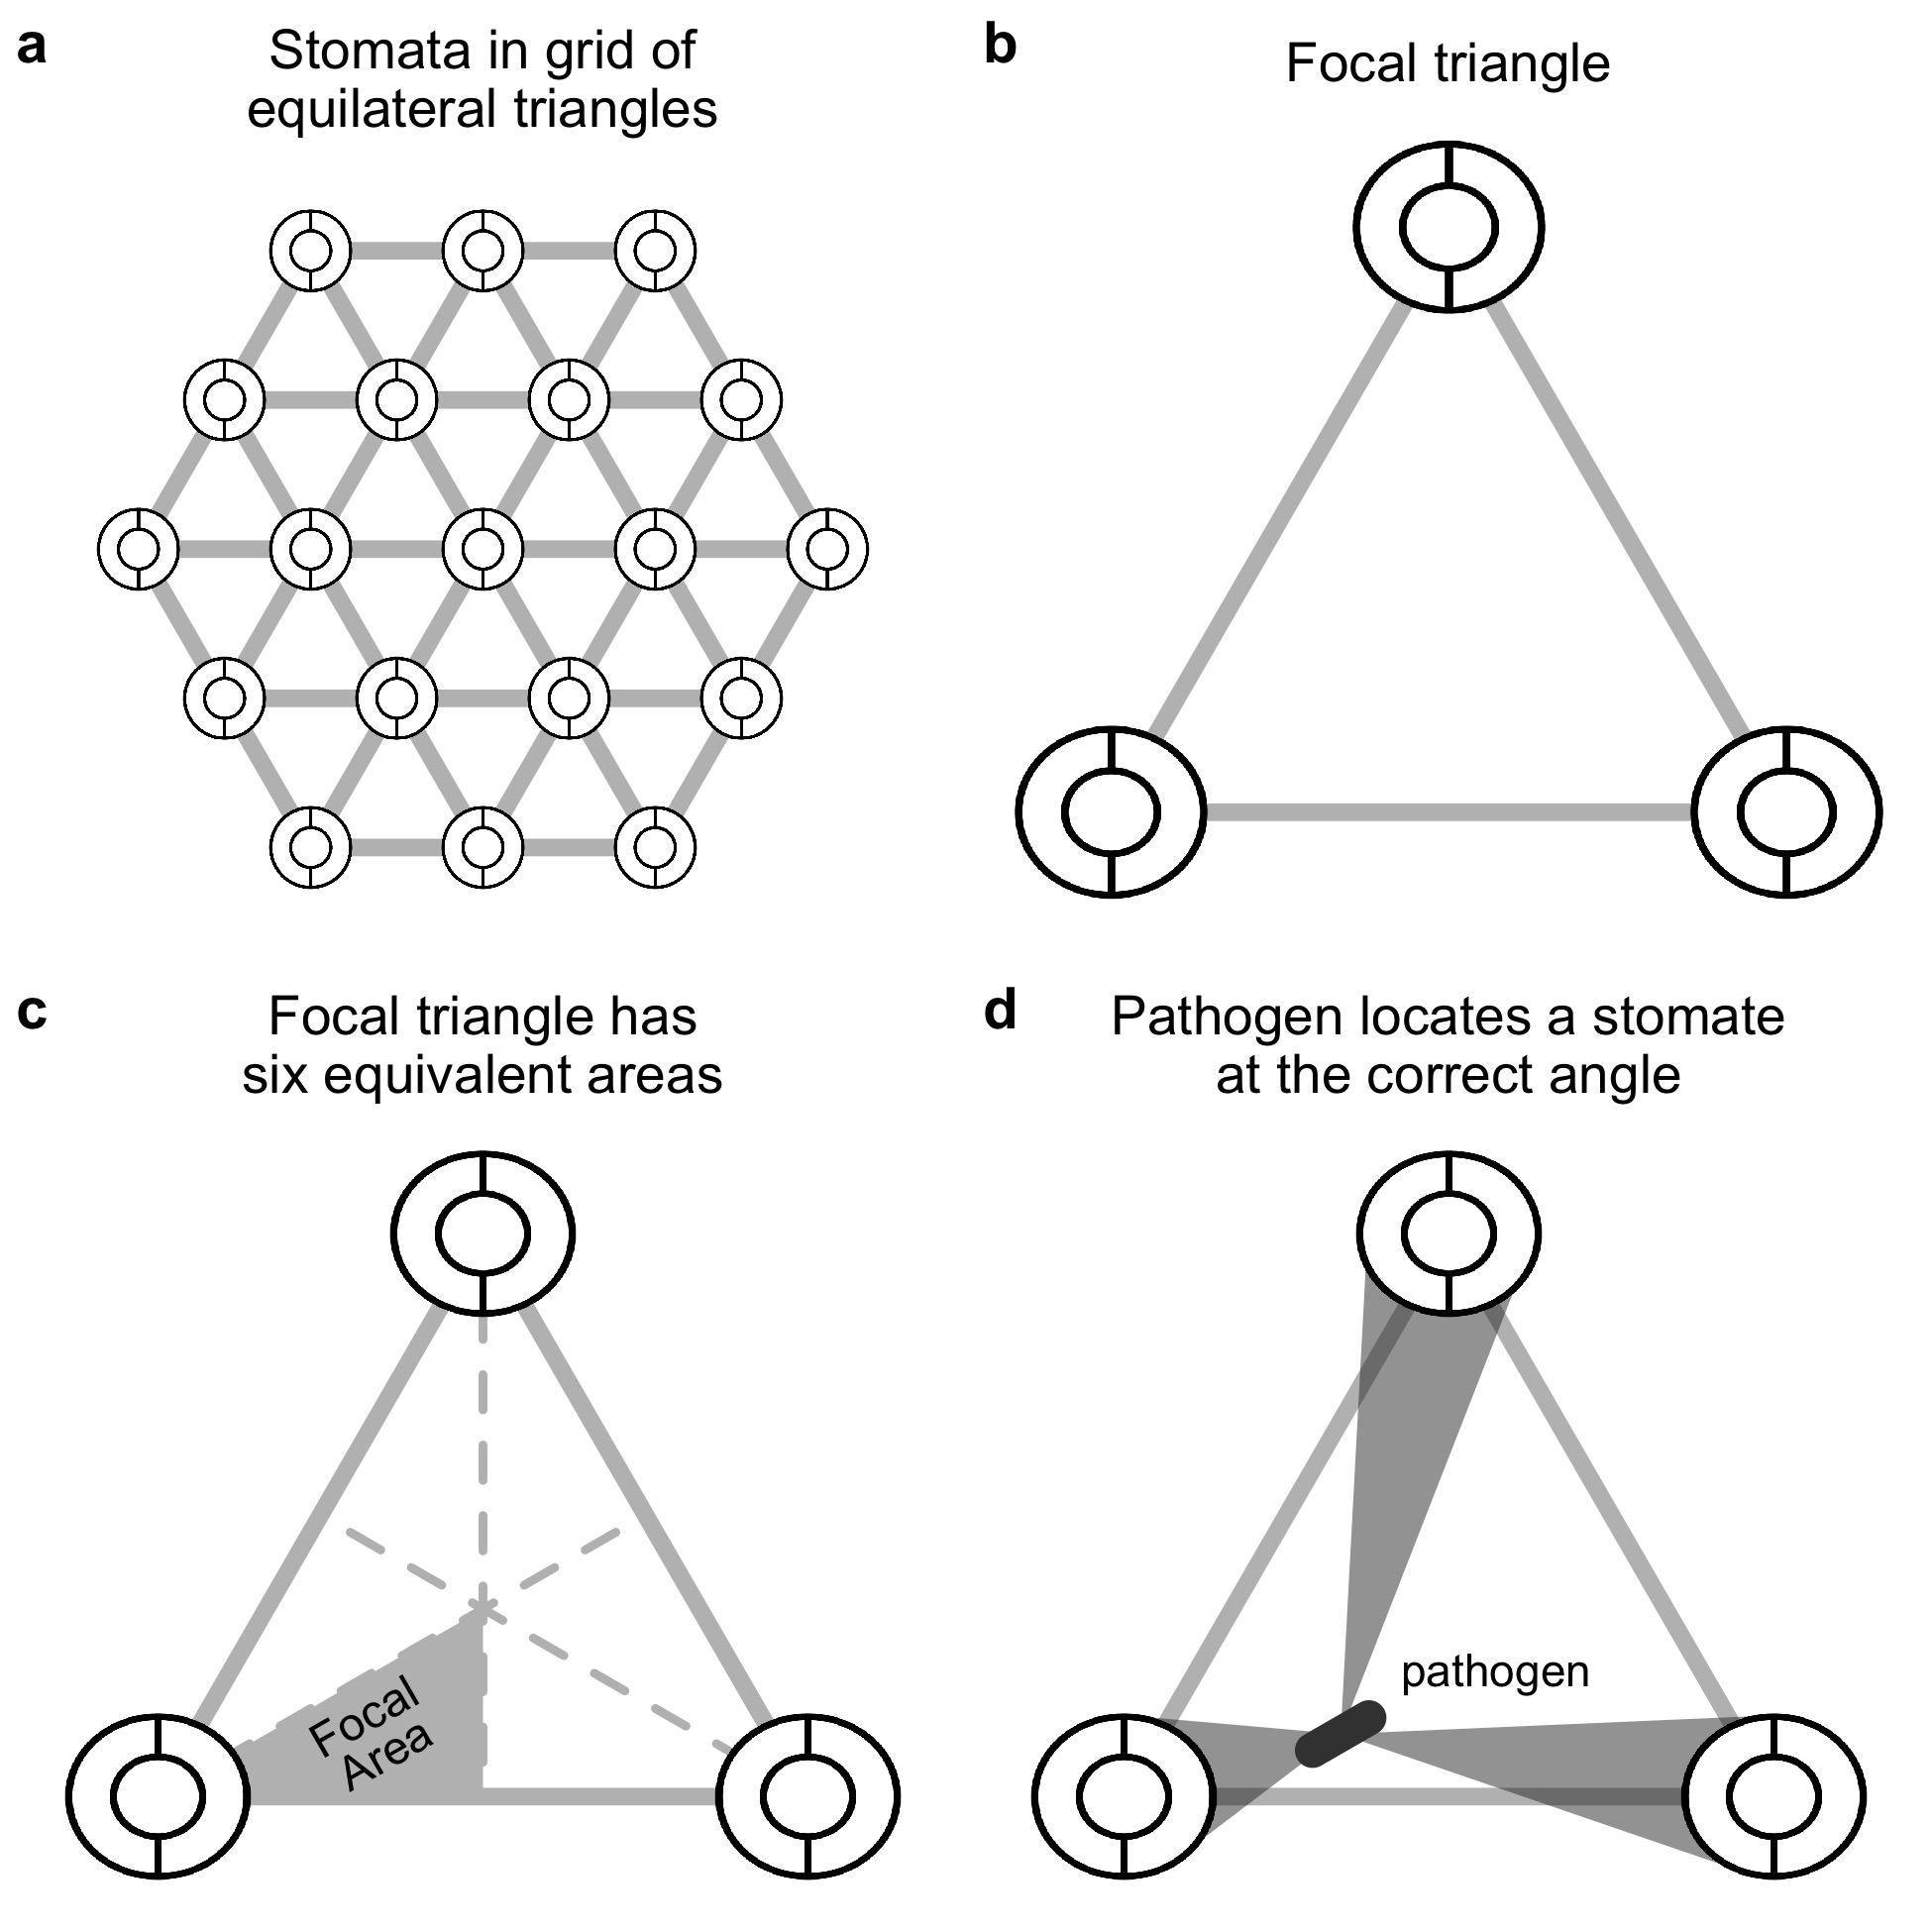
\includegraphics[width=6.5in]{../figures/fig1.jpeg}
    \caption{\textbf{A spatially explicit model of stomatal anatomy and pathogen colonization}. \textbf{a}. Stomata are assumed to be in a homogenous equilateral triangular grid, which means that we can extrapolate from \textbf{b.} a focal triangle to the entire leaf. The circles represent idealized stomata; the grey lines between them are for visualization. \textbf{c.} By symmetry, a single focal region within the focal triangle can be modeled and extrapolated to the rest of the triangle. \textbf{d.} The model assumes that a pathogen, depicted as a grey rod, lands somewhere on the leaf surface and will sucessfully locate a stomate if it moves at the correct angle, depicted by the grey polygons.}
    \label{fig:fig1}
\end{figure}

\hypertarget{spatial-representation-of-pathogen-search}{%
\subsection*{Spatial representation of pathogen
search}\label{spatial-representation-of-pathogen-search}}
\addcontentsline{toc}{subsection}{Spatial representation of pathogen
search}

Since stomata are arrayed in a homogeneous grid, we can focus on single
focal triangle (Figure \ref{fig:fig1}b-c). Suppose that an individual
pathogen (e.g.~bacterial cell or fungal spore) lands at a uniform random
position within the focal triangle and must arrive at a stomate to
colonize. If it lands on a stomate, then it infects the leaf with
probability 1; if it lands between stomata, then it infects the leaf
with probability \(p_\text{locate}\). This is the probability that it
locates a stomate, which I will derive below. The probabilities of
landing on or between a stomate are \fs{} and \(1 - f_S\), respectively.
Hence, the total probability of colonization is:

\begin{equation}
  \label{eq:p_colonize}
  p_\text{colonize} = f_\text{S} + (1 - f_\text{S}) p_\text{locate}.
\end{equation}

I assume that the pathogen cannot sense where stomata are and orients at
random, thereafter traveling in that direction. If it successfully
locates a stomate, it colonizes the leaf, but otherwise does not infect.
If there is a high density of stomata and/or large stomata, the
probability of locating a stomate increases. By assuming that stomata
form an equilateral triangular grid (see above), we can extrapolate what
happens in the focal triangle (Figure \ref{fig:fig1}b) by symmetry.
Further, since an equilateral triangle can be broken up into six
identical units (Figure \ref{fig:fig1}c), we can simply calculate
\(p_\text{locate}\) in this focal area. This implicitly assumes that the
probability of colonizing stomata outside the focal area is 0 because
they are too far away. This assumption may be unrealistic for larger
pathogens, such as fungi, whose hyphae can travel longer distances on
the leaf surface (Brand and Gow, 2012). In
\protect\hyperlink{appendix-1-spatially-implicit-model}{Appendix 1:
Spatially implicit model} I derive a simpler, but spatially
\emph{implicit} model that relaxes the assumption the pathogens must
colonize a stomate within their focal triangle.

Consider a pathogen that lands in position (\(x_p,y_p\)) within the
triangle. The centroid of the triangle is at position (\(x_c,y_c\)) and
a reference stomate is at position \((0,0)\) (Figure \ref{fig:fig2}a).
Therefore \(x_c = U / 2\) and \(y_c = \sqrt{3} U / 6\). The other
stomata are at positions \((U/2, \sqrt{3} U /2)\) and \((U,0)\) (Figure
\ref{fig:fig2}). \(x_p\) and \(y_p\) are defined as the horizontal and
vertical distances, respectively, from the pathogen to the reference
stomate at position \((0,0)\).

Given that the pathogen starts at position (\(x_p,y_p\)), what's the
probability of contacting one of the stomata at the vertices of the
focal triangle? I assume the probability of contacting a stomate is
equal to the proportion of angular directions that lead to a stomate
(Figure \ref{fig:fig1}d). I solved this by finding the angles
(\(\theta_1, \theta_2, \theta_3\)) between lines that are tangent to the
outside of the three stomata and pass through (\(x_p,y_p\)) (Figure
\ref{fig:fig2}a). If stomate \(i\) is centered at (\(x_i,y_i\)), the two
slopes of tangency as function of pathogen position are:

\begin{align}
  t_{i,1}(x_p,y_p) & = \frac{-R e_{i,2}(x_p,y_p) + e_{i,3}(x_p,y_p)}{e_{i,1}(x_p,y_p)} \\
  t_{i,2}(x_p,y_p) & = \frac{R e_{i,2}(x_p,y_p) + e_{i,3}(x_p,y_p)}{e_{i,1}(x_p,y_p)}
\end{align}

where

\begin{align}
  e_{i,1}(x_p,y_p) & = (R^2 - x_i^2 + 2 x_i x_p - x_p^2), \\
  e_{i,2}(x_p,y_p) & = \sqrt{-e_{i,1} + (y_i - y_p) ^ 2}, \\
  e_{i,3}(x_p,y_p) & = - x_i y_i + x_i y_p + x_p y_i - x_p y_p.
\end{align}

Note that \(i \in \{1, 2, 3\}\), indexing the three stomata in the focal
triangle. The angle in radians between \(t_{i,1}(x_p,y_p)\) and
\(t_{i,2}(x_p,y_p)\) is:

\begin{equation}
  \theta_i(x_p,y_p) = \text{arctan}\bigg(\frac{t_{i,1}(x_p,y_p) - t_{i,2}(x_p,y_p)}{1 + (t_{i,1}(x_p,y_p) t_{i,2}(x_p,y_p))}\bigg)
\end{equation}

\begin{figure}
\centering
% Created by tikzDevice version 0.12.3.1 on 2020-10-17 14:52:20
% !TEX encoding = UTF-8 Unicode
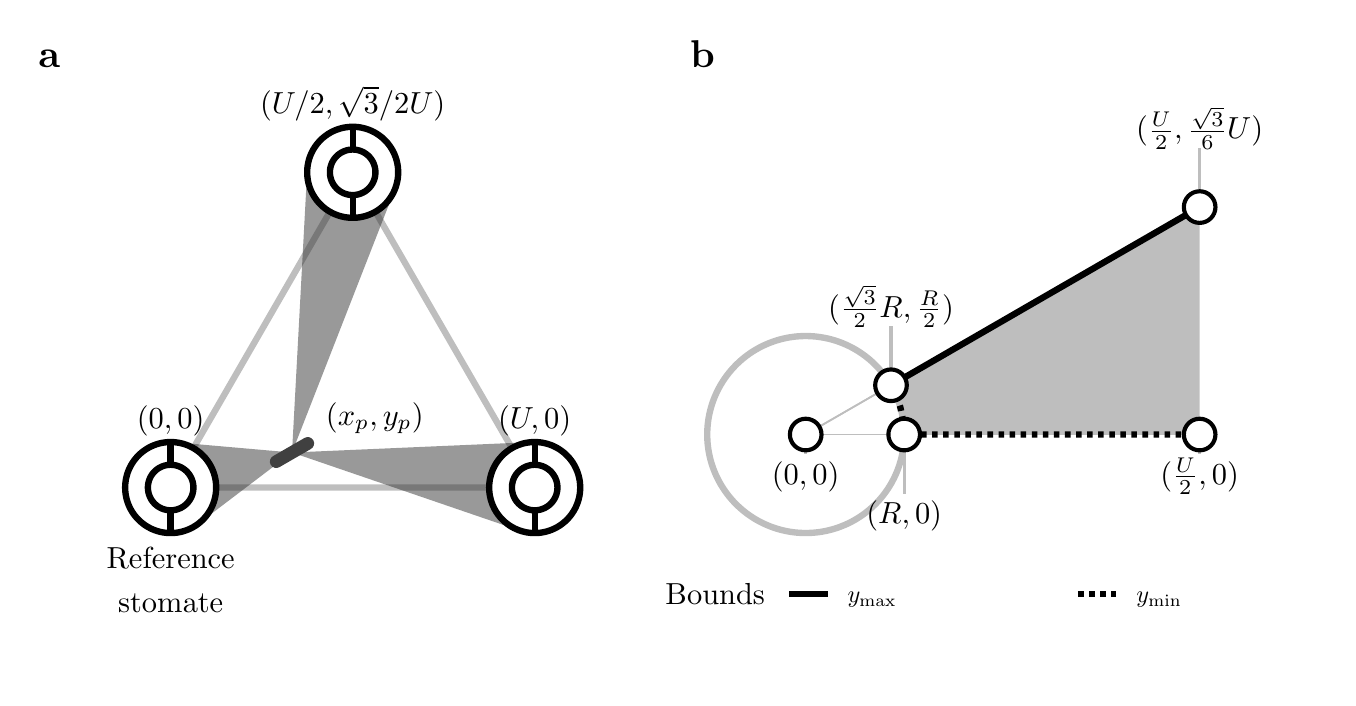
\begin{tikzpicture}[x=1pt,y=1pt]
\definecolor{fillColor}{RGB}{255,255,255}
\path[use as bounding box,fill=fillColor,fill opacity=0.00] (0,0) rectangle (469.75,234.88);
\begin{scope}
\path[clip] ( 14.68,  0.00) rectangle (220.20,234.88);
\definecolor{drawColor}{RGB}{190,190,190}

\path[draw=drawColor,line width= 2.3pt,line join=round,line cap=round] ( 51.67, 68.70) --
	(183.21, 68.70) --
	(117.44,182.62) --
	( 51.67, 68.70);
\definecolor{fillColor}{RGB}{51,51,51}

\path[fill=fillColor,fill opacity=0.50] ( 95.52, 81.36) --
	(101.02,183.50) --
	(132.75,176.63) --
	( 95.52, 81.36) --
	cycle;

\path[fill=fillColor,fill opacity=0.50] ( 95.52, 81.36) --
	( 61.62, 55.61) --
	( 53.11, 85.08) --
	( 95.52, 81.36) --
	cycle;

\path[fill=fillColor,fill opacity=0.50] ( 95.52, 81.36) --
	(182.49, 85.13) --
	(177.88, 53.15) --
	( 95.52, 81.36) --
	cycle;
\definecolor{drawColor}{gray}{0.25}

\path[draw=drawColor,line width= 4.6pt,line join=round,line cap=round] ( 89.82, 78.07) -- (101.21, 84.65);
\definecolor{drawColor}{RGB}{0,0,0}

\node[text=drawColor,anchor=base west,inner sep=0pt, outer sep=0pt, scale=  1.10] at (107.79, 91.23) {$(x_p, y_p)$};

\node[text=drawColor,anchor=base,inner sep=0pt, outer sep=0pt, scale=  1.10] at (117.44,203.79) {$(U/2, \sqrt{3} / 2 U)$};

\node[text=drawColor,anchor=base,inner sep=0pt, outer sep=0pt, scale=  1.10] at ( 51.67, 89.87) {$(0, 0)$};

\node[text=drawColor,anchor=base,inner sep=0pt, outer sep=0pt, scale=  1.10] at (183.21, 89.87) {$(U, 0)$};

\node[text=drawColor,anchor=base,inner sep=0pt, outer sep=0pt, scale=  1.10] at ( 51.67, 39.38) {Reference};

\node[text=drawColor,anchor=base,inner sep=0pt, outer sep=0pt, scale=  1.10] at ( 51.67, 23.49) {stomate};
\definecolor{fillColor}{RGB}{255,255,255}

\path[draw=drawColor,line width= 2.3pt,line join=round,line cap=round,fill=fillColor] (117.44,199.06) --
	(117.73,199.06) --
	(118.01,199.05) --
	(118.30,199.04) --
	(118.59,199.02) --
	(118.87,199.00) --
	(119.16,198.97) --
	(119.44,198.94) --
	(119.73,198.90) --
	(120.01,198.86) --
	(120.29,198.81) --
	(120.58,198.76) --
	(120.86,198.70) --
	(121.14,198.64) --
	(121.42,198.57) --
	(121.69,198.50) --
	(121.97,198.42) --
	(122.25,198.34) --
	(122.52,198.25) --
	(122.79,198.16) --
	(123.06,198.07) --
	(123.33,197.97) --
	(123.60,197.86) --
	(123.86,197.75) --
	(124.13,197.64) --
	(124.39,197.52) --
	(124.65,197.39) --
	(124.90,197.27) --
	(125.16,197.13) --
	(125.41,197.00) --
	(125.66,196.86) --
	(125.91,196.71) --
	(126.15,196.56) --
	(126.39,196.41) --
	(126.63,196.25) --
	(126.87,196.08) --
	(127.10,195.92) --
	(127.33,195.75) --
	(127.56,195.57) --
	(127.79,195.39) --
	(128.01,195.21) --
	(128.23,195.03) --
	(128.44,194.84) --
	(128.65,194.64) --
	(128.86,194.44) --
	(129.06,194.24) --
	(129.27,194.04) --
	(129.46,193.83) --
	(129.66,193.62) --
	(129.85,193.40) --
	(130.03,193.19) --
	(130.22,192.96) --
	(130.40,192.74) --
	(130.57,192.51) --
	(130.74,192.28) --
	(130.91,192.05) --
	(131.07,191.81) --
	(131.23,191.57) --
	(131.38,191.33) --
	(131.53,191.08) --
	(131.68,190.84) --
	(131.82,190.59) --
	(131.96,190.34) --
	(132.09,190.08) --
	(132.22,189.82) --
	(132.34,189.56) --
	(132.46,189.30) --
	(132.57,189.04) --
	(132.68,188.78) --
	(132.79,188.51) --
	(132.89,188.24) --
	(132.98,187.97) --
	(133.08,187.70) --
	(133.16,187.42) --
	(133.24,187.15) --
	(133.32,186.87) --
	(133.39,186.59) --
	(133.46,186.31) --
	(133.52,186.03) --
	(133.58,185.75) --
	(133.63,185.47) --
	(133.68,185.19) --
	(133.72,184.90) --
	(133.76,184.62) --
	(133.79,184.33) --
	(133.82,184.05) --
	(133.84,183.76) --
	(133.86,183.48) --
	(133.87,183.19) --
	(133.88,182.90) --
	(133.88,182.62) --
	(133.88,182.33) --
	(133.87,182.04) --
	(133.86,181.76) --
	(133.84,181.47) --
	(133.82,181.18) --
	(133.79,180.90) --
	(133.76,180.61) --
	(133.72,180.33) --
	(133.68,180.04) --
	(133.63,179.76) --
	(133.58,179.48) --
	(133.52,179.20) --
	(133.46,178.92) --
	(133.39,178.64) --
	(133.32,178.36) --
	(133.24,178.08) --
	(133.16,177.81) --
	(133.08,177.54) --
	(132.98,177.26) --
	(132.89,176.99) --
	(132.79,176.72) --
	(132.68,176.46) --
	(132.57,176.19) --
	(132.46,175.93) --
	(132.34,175.67) --
	(132.22,175.41) --
	(132.09,175.15) --
	(131.96,174.90) --
	(131.82,174.65) --
	(131.68,174.40) --
	(131.53,174.15) --
	(131.38,173.90) --
	(131.23,173.66) --
	(131.07,173.42) --
	(130.91,173.19) --
	(130.74,172.95) --
	(130.57,172.72) --
	(130.40,172.49) --
	(130.22,172.27) --
	(130.03,172.05) --
	(129.85,171.83) --
	(129.66,171.61) --
	(129.46,171.40) --
	(129.27,171.19) --
	(129.06,170.99) --
	(128.86,170.79) --
	(128.65,170.59) --
	(128.44,170.40) --
	(128.23,170.21) --
	(128.01,170.02) --
	(127.79,169.84) --
	(127.56,169.66) --
	(127.33,169.49) --
	(127.10,169.31) --
	(126.87,169.15) --
	(126.63,168.99) --
	(126.39,168.83) --
	(126.15,168.67) --
	(125.91,168.52) --
	(125.66,168.38) --
	(125.41,168.24) --
	(125.16,168.10) --
	(124.90,167.97) --
	(124.65,167.84) --
	(124.39,167.71) --
	(124.13,167.60) --
	(123.86,167.48) --
	(123.60,167.37) --
	(123.33,167.27) --
	(123.06,167.17) --
	(122.79,167.07) --
	(122.52,166.98) --
	(122.25,166.89) --
	(121.97,166.81) --
	(121.69,166.73) --
	(121.42,166.66) --
	(121.14,166.60) --
	(120.86,166.53) --
	(120.58,166.48) --
	(120.29,166.42) --
	(120.01,166.38) --
	(119.73,166.33) --
	(119.44,166.30) --
	(119.16,166.26) --
	(118.87,166.24) --
	(118.59,166.21) --
	(118.30,166.20) --
	(118.01,166.18) --
	(117.73,166.18) --
	(117.44,166.17) --
	(117.15,166.18) --
	(116.86,166.18) --
	(116.58,166.20) --
	(116.29,166.21) --
	(116.01,166.24) --
	(115.72,166.26) --
	(115.43,166.30) --
	(115.15,166.33) --
	(114.87,166.38) --
	(114.58,166.42) --
	(114.30,166.48) --
	(114.02,166.53) --
	(113.74,166.60) --
	(113.46,166.66) --
	(113.18,166.73) --
	(112.91,166.81) --
	(112.63,166.89) --
	(112.36,166.98) --
	(112.09,167.07) --
	(111.82,167.17) --
	(111.55,167.27) --
	(111.28,167.37) --
	(111.01,167.48) --
	(110.75,167.60) --
	(110.49,167.71) --
	(110.23,167.84) --
	(109.97,167.97) --
	(109.72,168.10) --
	(109.47,168.24) --
	(109.22,168.38) --
	(108.97,168.52) --
	(108.73,168.67) --
	(108.48,168.83) --
	(108.24,168.99) --
	(108.01,169.15) --
	(107.77,169.31) --
	(107.54,169.49) --
	(107.32,169.66) --
	(107.09,169.84) --
	(106.87,170.02) --
	(106.65,170.21) --
	(106.44,170.40) --
	(106.23,170.59) --
	(106.02,170.79) --
	(105.81,170.99) --
	(105.61,171.19) --
	(105.41,171.40) --
	(105.22,171.61) --
	(105.03,171.83) --
	(104.84,172.05) --
	(104.66,172.27) --
	(104.48,172.49) --
	(104.31,172.72) --
	(104.14,172.95) --
	(103.97,173.19) --
	(103.81,173.42) --
	(103.65,173.66) --
	(103.50,173.90) --
	(103.35,174.15) --
	(103.20,174.40) --
	(103.06,174.65) --
	(102.92,174.90) --
	(102.79,175.15) --
	(102.66,175.41) --
	(102.54,175.67) --
	(102.42,175.93) --
	(102.30,176.19) --
	(102.19,176.46) --
	(102.09,176.72) --
	(101.99,176.99) --
	(101.89,177.26) --
	(101.80,177.54) --
	(101.72,177.81) --
	(101.63,178.08) --
	(101.56,178.36) --
	(101.49,178.64) --
	(101.42,178.92) --
	(101.36,179.20) --
	(101.30,179.48) --
	(101.25,179.76) --
	(101.20,180.04) --
	(101.16,180.33) --
	(101.12,180.61) --
	(101.09,180.90) --
	(101.06,181.18) --
	(101.04,181.47) --
	(101.02,181.76) --
	(101.01,182.04) --
	(101.00,182.33) --
	(101.00,182.62) --
	(101.00,182.90) --
	(101.01,183.19) --
	(101.02,183.48) --
	(101.04,183.76) --
	(101.06,184.05) --
	(101.09,184.33) --
	(101.12,184.62) --
	(101.16,184.90) --
	(101.20,185.19) --
	(101.25,185.47) --
	(101.30,185.75) --
	(101.36,186.03) --
	(101.42,186.31) --
	(101.49,186.59) --
	(101.56,186.87) --
	(101.63,187.15) --
	(101.72,187.42) --
	(101.80,187.70) --
	(101.89,187.97) --
	(101.99,188.24) --
	(102.09,188.51) --
	(102.19,188.78) --
	(102.30,189.04) --
	(102.42,189.30) --
	(102.54,189.56) --
	(102.66,189.82) --
	(102.79,190.08) --
	(102.92,190.34) --
	(103.06,190.59) --
	(103.20,190.84) --
	(103.35,191.08) --
	(103.50,191.33) --
	(103.65,191.57) --
	(103.81,191.81) --
	(103.97,192.05) --
	(104.14,192.28) --
	(104.31,192.51) --
	(104.48,192.74) --
	(104.66,192.96) --
	(104.84,193.19) --
	(105.03,193.40) --
	(105.22,193.62) --
	(105.41,193.83) --
	(105.61,194.04) --
	(105.81,194.24) --
	(106.02,194.44) --
	(106.23,194.64) --
	(106.44,194.84) --
	(106.65,195.03) --
	(106.87,195.21) --
	(107.09,195.39) --
	(107.32,195.57) --
	(107.54,195.75) --
	(107.77,195.92) --
	(108.01,196.08) --
	(108.24,196.25) --
	(108.48,196.41) --
	(108.73,196.56) --
	(108.97,196.71) --
	(109.22,196.86) --
	(109.47,197.00) --
	(109.72,197.13) --
	(109.97,197.27) --
	(110.23,197.39) --
	(110.49,197.52) --
	(110.75,197.64) --
	(111.01,197.75) --
	(111.28,197.86) --
	(111.55,197.97) --
	(111.82,198.07) --
	(112.09,198.16) --
	(112.36,198.25) --
	(112.63,198.34) --
	(112.91,198.42) --
	(113.18,198.50) --
	(113.46,198.57) --
	(113.74,198.64) --
	(114.02,198.70) --
	(114.30,198.76) --
	(114.58,198.81) --
	(114.87,198.86) --
	(115.15,198.90) --
	(115.43,198.94) --
	(115.72,198.97) --
	(116.01,199.00) --
	(116.29,199.02) --
	(116.58,199.04) --
	(116.86,199.05) --
	(117.15,199.06) --
	(117.44,199.06) --
	cycle;

\path[draw=drawColor,line width= 2.3pt,line join=round,line cap=round,fill=fillColor] ( 51.67, 85.15) --
	( 51.96, 85.14) --
	( 52.24, 85.14) --
	( 52.53, 85.12) --
	( 52.82, 85.11) --
	( 53.10, 85.08) --
	( 53.39, 85.06) --
	( 53.67, 85.02) --
	( 53.96, 84.99) --
	( 54.24, 84.94) --
	( 54.53, 84.90) --
	( 54.81, 84.84) --
	( 55.09, 84.79) --
	( 55.37, 84.72) --
	( 55.65, 84.66) --
	( 55.93, 84.58) --
	( 56.20, 84.51) --
	( 56.48, 84.43) --
	( 56.75, 84.34) --
	( 57.02, 84.25) --
	( 57.29, 84.15) --
	( 57.56, 84.05) --
	( 57.83, 83.95) --
	( 58.10, 83.84) --
	( 58.36, 83.72) --
	( 58.62, 83.60) --
	( 58.88, 83.48) --
	( 59.14, 83.35) --
	( 59.39, 83.22) --
	( 59.64, 83.08) --
	( 59.89, 82.94) --
	( 60.14, 82.80) --
	( 60.38, 82.65) --
	( 60.63, 82.49) --
	( 60.87, 82.33) --
	( 61.10, 82.17) --
	( 61.34, 82.00) --
	( 61.57, 81.83) --
	( 61.79, 81.66) --
	( 62.02, 81.48) --
	( 62.24, 81.30) --
	( 62.46, 81.11) --
	( 62.67, 80.92) --
	( 62.88, 80.73) --
	( 63.09, 80.53) --
	( 63.30, 80.33) --
	( 63.50, 80.12) --
	( 63.70, 79.92) --
	( 63.89, 79.70) --
	( 64.08, 79.49) --
	( 64.27, 79.27) --
	( 64.45, 79.05) --
	( 64.63, 78.83) --
	( 64.80, 78.60) --
	( 64.97, 78.37) --
	( 65.14, 78.13) --
	( 65.30, 77.90) --
	( 65.46, 77.66) --
	( 65.61, 77.42) --
	( 65.76, 77.17) --
	( 65.91, 76.92) --
	( 66.05, 76.67) --
	( 66.19, 76.42) --
	( 66.32, 76.17) --
	( 66.45, 75.91) --
	( 66.57, 75.65) --
	( 66.69, 75.39) --
	( 66.81, 75.13) --
	( 66.92, 74.86) --
	( 67.02, 74.60) --
	( 67.12, 74.33) --
	( 67.22, 74.06) --
	( 67.31, 73.78) --
	( 67.39, 73.51) --
	( 67.48, 73.24) --
	( 67.55, 72.96) --
	( 67.62, 72.68) --
	( 67.69, 72.40) --
	( 67.75, 72.12) --
	( 67.81, 71.84) --
	( 67.86, 71.56) --
	( 67.91, 71.28) --
	( 67.95, 70.99) --
	( 67.99, 70.71) --
	( 68.02, 70.42) --
	( 68.05, 70.14) --
	( 68.07, 69.85) --
	( 68.09, 69.56) --
	( 68.10, 69.28) --
	( 68.11, 68.99) --
	( 68.11, 68.70) --
	( 68.11, 68.42) --
	( 68.10, 68.13) --
	( 68.09, 67.84) --
	( 68.07, 67.56) --
	( 68.05, 67.27) --
	( 68.02, 66.98) --
	( 67.99, 66.70) --
	( 67.95, 66.41) --
	( 67.91, 66.13) --
	( 67.86, 65.85) --
	( 67.81, 65.57) --
	( 67.75, 65.28) --
	( 67.69, 65.00) --
	( 67.62, 64.73) --
	( 67.55, 64.45) --
	( 67.48, 64.17) --
	( 67.39, 63.90) --
	( 67.31, 63.62) --
	( 67.22, 63.35) --
	( 67.12, 63.08) --
	( 67.02, 62.81) --
	( 66.92, 62.54) --
	( 66.81, 62.28) --
	( 66.69, 62.02) --
	( 66.57, 61.75) --
	( 66.45, 61.50) --
	( 66.32, 61.24) --
	( 66.19, 60.98) --
	( 66.05, 60.73) --
	( 65.91, 60.48) --
	( 65.76, 60.23) --
	( 65.61, 59.99) --
	( 65.46, 59.75) --
	( 65.30, 59.51) --
	( 65.14, 59.27) --
	( 64.97, 59.04) --
	( 64.80, 58.81) --
	( 64.63, 58.58) --
	( 64.45, 58.36) --
	( 64.27, 58.13) --
	( 64.08, 57.92) --
	( 63.89, 57.70) --
	( 63.70, 57.49) --
	( 63.50, 57.28) --
	( 63.30, 57.08) --
	( 63.09, 56.88) --
	( 62.88, 56.68) --
	( 62.67, 56.48) --
	( 62.46, 56.29) --
	( 62.24, 56.11) --
	( 62.02, 55.93) --
	( 61.79, 55.75) --
	( 61.57, 55.57) --
	( 61.34, 55.40) --
	( 61.10, 55.23) --
	( 60.87, 55.07) --
	( 60.63, 54.91) --
	( 60.38, 54.76) --
	( 60.14, 54.61) --
	( 59.89, 54.46) --
	( 59.64, 54.32) --
	( 59.39, 54.19) --
	( 59.14, 54.05) --
	( 58.88, 53.93) --
	( 58.62, 53.80) --
	( 58.36, 53.68) --
	( 58.10, 53.57) --
	( 57.83, 53.46) --
	( 57.56, 53.35) --
	( 57.29, 53.25) --
	( 57.02, 53.16) --
	( 56.75, 53.07) --
	( 56.48, 52.98) --
	( 56.20, 52.90) --
	( 55.93, 52.82) --
	( 55.65, 52.75) --
	( 55.37, 52.68) --
	( 55.09, 52.62) --
	( 54.81, 52.56) --
	( 54.53, 52.51) --
	( 54.24, 52.46) --
	( 53.96, 52.42) --
	( 53.67, 52.38) --
	( 53.39, 52.35) --
	( 53.10, 52.32) --
	( 52.82, 52.30) --
	( 52.53, 52.28) --
	( 52.24, 52.27) --
	( 51.96, 52.26) --
	( 51.67, 52.26) --
	( 51.38, 52.26) --
	( 51.10, 52.27) --
	( 50.81, 52.28) --
	( 50.52, 52.30) --
	( 50.24, 52.32) --
	( 49.95, 52.35) --
	( 49.67, 52.38) --
	( 49.38, 52.42) --
	( 49.10, 52.46) --
	( 48.82, 52.51) --
	( 48.53, 52.56) --
	( 48.25, 52.62) --
	( 47.97, 52.68) --
	( 47.69, 52.75) --
	( 47.42, 52.82) --
	( 47.14, 52.90) --
	( 46.86, 52.98) --
	( 46.59, 53.07) --
	( 46.32, 53.16) --
	( 46.05, 53.25) --
	( 45.78, 53.35) --
	( 45.51, 53.46) --
	( 45.25, 53.57) --
	( 44.98, 53.68) --
	( 44.72, 53.80) --
	( 44.46, 53.93) --
	( 44.21, 54.05) --
	( 43.95, 54.19) --
	( 43.70, 54.32) --
	( 43.45, 54.46) --
	( 43.20, 54.61) --
	( 42.96, 54.76) --
	( 42.72, 54.91) --
	( 42.48, 55.07) --
	( 42.24, 55.23) --
	( 42.01, 55.40) --
	( 41.78, 55.57) --
	( 41.55, 55.75) --
	( 41.32, 55.93) --
	( 41.10, 56.11) --
	( 40.88, 56.29) --
	( 40.67, 56.48) --
	( 40.46, 56.68) --
	( 40.25, 56.88) --
	( 40.04, 57.08) --
	( 39.84, 57.28) --
	( 39.65, 57.49) --
	( 39.45, 57.70) --
	( 39.26, 57.92) --
	( 39.08, 58.13) --
	( 38.89, 58.36) --
	( 38.71, 58.58) --
	( 38.54, 58.81) --
	( 38.37, 59.04) --
	( 38.20, 59.27) --
	( 38.04, 59.51) --
	( 37.88, 59.75) --
	( 37.73, 59.99) --
	( 37.58, 60.23) --
	( 37.43, 60.48) --
	( 37.29, 60.73) --
	( 37.15, 60.98) --
	( 37.02, 61.24) --
	( 36.89, 61.50) --
	( 36.77, 61.75) --
	( 36.65, 62.02) --
	( 36.54, 62.28) --
	( 36.43, 62.54) --
	( 36.32, 62.81) --
	( 36.22, 63.08) --
	( 36.12, 63.35) --
	( 36.03, 63.62) --
	( 35.95, 63.90) --
	( 35.87, 64.17) --
	( 35.79, 64.45) --
	( 35.72, 64.73) --
	( 35.65, 65.00) --
	( 35.59, 65.28) --
	( 35.53, 65.57) --
	( 35.48, 65.85) --
	( 35.43, 66.13) --
	( 35.39, 66.41) --
	( 35.35, 66.70) --
	( 35.32, 66.98) --
	( 35.29, 67.27) --
	( 35.27, 67.56) --
	( 35.25, 67.84) --
	( 35.24, 68.13) --
	( 35.23, 68.42) --
	( 35.23, 68.70) --
	( 35.23, 68.99) --
	( 35.24, 69.28) --
	( 35.25, 69.56) --
	( 35.27, 69.85) --
	( 35.29, 70.14) --
	( 35.32, 70.42) --
	( 35.35, 70.71) --
	( 35.39, 70.99) --
	( 35.43, 71.28) --
	( 35.48, 71.56) --
	( 35.53, 71.84) --
	( 35.59, 72.12) --
	( 35.65, 72.40) --
	( 35.72, 72.68) --
	( 35.79, 72.96) --
	( 35.87, 73.24) --
	( 35.95, 73.51) --
	( 36.03, 73.78) --
	( 36.12, 74.06) --
	( 36.22, 74.33) --
	( 36.32, 74.60) --
	( 36.43, 74.86) --
	( 36.54, 75.13) --
	( 36.65, 75.39) --
	( 36.77, 75.65) --
	( 36.89, 75.91) --
	( 37.02, 76.17) --
	( 37.15, 76.42) --
	( 37.29, 76.67) --
	( 37.43, 76.92) --
	( 37.58, 77.17) --
	( 37.73, 77.42) --
	( 37.88, 77.66) --
	( 38.04, 77.90) --
	( 38.20, 78.13) --
	( 38.37, 78.37) --
	( 38.54, 78.60) --
	( 38.71, 78.83) --
	( 38.89, 79.05) --
	( 39.08, 79.27) --
	( 39.26, 79.49) --
	( 39.45, 79.70) --
	( 39.65, 79.92) --
	( 39.84, 80.12) --
	( 40.04, 80.33) --
	( 40.25, 80.53) --
	( 40.46, 80.73) --
	( 40.67, 80.92) --
	( 40.88, 81.11) --
	( 41.10, 81.30) --
	( 41.32, 81.48) --
	( 41.55, 81.66) --
	( 41.78, 81.83) --
	( 42.01, 82.00) --
	( 42.24, 82.17) --
	( 42.48, 82.33) --
	( 42.72, 82.49) --
	( 42.96, 82.65) --
	( 43.20, 82.80) --
	( 43.45, 82.94) --
	( 43.70, 83.08) --
	( 43.95, 83.22) --
	( 44.21, 83.35) --
	( 44.46, 83.48) --
	( 44.72, 83.60) --
	( 44.98, 83.72) --
	( 45.25, 83.84) --
	( 45.51, 83.95) --
	( 45.78, 84.05) --
	( 46.05, 84.15) --
	( 46.32, 84.25) --
	( 46.59, 84.34) --
	( 46.86, 84.43) --
	( 47.14, 84.51) --
	( 47.42, 84.58) --
	( 47.69, 84.66) --
	( 47.97, 84.72) --
	( 48.25, 84.79) --
	( 48.53, 84.84) --
	( 48.82, 84.90) --
	( 49.10, 84.94) --
	( 49.38, 84.99) --
	( 49.67, 85.02) --
	( 49.95, 85.06) --
	( 50.24, 85.08) --
	( 50.52, 85.11) --
	( 50.81, 85.12) --
	( 51.10, 85.14) --
	( 51.38, 85.14) --
	( 51.67, 85.15) --
	cycle;

\path[draw=drawColor,line width= 2.3pt,line join=round,line cap=round,fill=fillColor] (183.21, 85.15) --
	(183.49, 85.14) --
	(183.78, 85.14) --
	(184.07, 85.12) --
	(184.35, 85.11) --
	(184.64, 85.08) --
	(184.93, 85.06) --
	(185.21, 85.02) --
	(185.49, 84.99) --
	(185.78, 84.94) --
	(186.06, 84.90) --
	(186.34, 84.84) --
	(186.63, 84.79) --
	(186.91, 84.72) --
	(187.18, 84.66) --
	(187.46, 84.58) --
	(187.74, 84.51) --
	(188.01, 84.43) --
	(188.29, 84.34) --
	(188.56, 84.25) --
	(188.83, 84.15) --
	(189.10, 84.05) --
	(189.37, 83.95) --
	(189.63, 83.84) --
	(189.89, 83.72) --
	(190.16, 83.60) --
	(190.41, 83.48) --
	(190.67, 83.35) --
	(190.93, 83.22) --
	(191.18, 83.08) --
	(191.43, 82.94) --
	(191.67, 82.80) --
	(191.92, 82.65) --
	(192.16, 82.49) --
	(192.40, 82.33) --
	(192.64, 82.17) --
	(192.87, 82.00) --
	(193.10, 81.83) --
	(193.33, 81.66) --
	(193.55, 81.48) --
	(193.78, 81.30) --
	(193.99, 81.11) --
	(194.21, 80.92) --
	(194.42, 80.73) --
	(194.63, 80.53) --
	(194.83, 80.33) --
	(195.03, 80.12) --
	(195.23, 79.92) --
	(195.43, 79.70) --
	(195.62, 79.49) --
	(195.80, 79.27) --
	(195.98, 79.05) --
	(196.16, 78.83) --
	(196.34, 78.60) --
	(196.51, 78.37) --
	(196.68, 78.13) --
	(196.84, 77.90) --
	(197.00, 77.66) --
	(197.15, 77.42) --
	(197.30, 77.17) --
	(197.45, 76.92) --
	(197.59, 76.67) --
	(197.72, 76.42) --
	(197.86, 76.17) --
	(197.98, 75.91) --
	(198.11, 75.65) --
	(198.23, 75.39) --
	(198.34, 75.13) --
	(198.45, 74.86) --
	(198.56, 74.60) --
	(198.66, 74.33) --
	(198.75, 74.06) --
	(198.84, 73.78) --
	(198.93, 73.51) --
	(199.01, 73.24) --
	(199.09, 72.96) --
	(199.16, 72.68) --
	(199.23, 72.40) --
	(199.29, 72.12) --
	(199.35, 71.84) --
	(199.40, 71.56) --
	(199.45, 71.28) --
	(199.49, 70.99) --
	(199.53, 70.71) --
	(199.56, 70.42) --
	(199.59, 70.14) --
	(199.61, 69.85) --
	(199.63, 69.56) --
	(199.64, 69.28) --
	(199.65, 68.99) --
	(199.65, 68.70) --
	(199.65, 68.42) --
	(199.64, 68.13) --
	(199.63, 67.84) --
	(199.61, 67.56) --
	(199.59, 67.27) --
	(199.56, 66.98) --
	(199.53, 66.70) --
	(199.49, 66.41) --
	(199.45, 66.13) --
	(199.40, 65.85) --
	(199.35, 65.57) --
	(199.29, 65.28) --
	(199.23, 65.00) --
	(199.16, 64.73) --
	(199.09, 64.45) --
	(199.01, 64.17) --
	(198.93, 63.90) --
	(198.84, 63.62) --
	(198.75, 63.35) --
	(198.66, 63.08) --
	(198.56, 62.81) --
	(198.45, 62.54) --
	(198.34, 62.28) --
	(198.23, 62.02) --
	(198.11, 61.75) --
	(197.98, 61.50) --
	(197.86, 61.24) --
	(197.72, 60.98) --
	(197.59, 60.73) --
	(197.45, 60.48) --
	(197.30, 60.23) --
	(197.15, 59.99) --
	(197.00, 59.75) --
	(196.84, 59.51) --
	(196.68, 59.27) --
	(196.51, 59.04) --
	(196.34, 58.81) --
	(196.16, 58.58) --
	(195.98, 58.36) --
	(195.80, 58.13) --
	(195.62, 57.92) --
	(195.43, 57.70) --
	(195.23, 57.49) --
	(195.03, 57.28) --
	(194.83, 57.08) --
	(194.63, 56.88) --
	(194.42, 56.68) --
	(194.21, 56.48) --
	(193.99, 56.29) --
	(193.78, 56.11) --
	(193.55, 55.93) --
	(193.33, 55.75) --
	(193.10, 55.57) --
	(192.87, 55.40) --
	(192.64, 55.23) --
	(192.40, 55.07) --
	(192.16, 54.91) --
	(191.92, 54.76) --
	(191.67, 54.61) --
	(191.43, 54.46) --
	(191.18, 54.32) --
	(190.93, 54.19) --
	(190.67, 54.05) --
	(190.41, 53.93) --
	(190.16, 53.80) --
	(189.89, 53.68) --
	(189.63, 53.57) --
	(189.37, 53.46) --
	(189.10, 53.35) --
	(188.83, 53.25) --
	(188.56, 53.16) --
	(188.29, 53.07) --
	(188.01, 52.98) --
	(187.74, 52.90) --
	(187.46, 52.82) --
	(187.18, 52.75) --
	(186.91, 52.68) --
	(186.63, 52.62) --
	(186.34, 52.56) --
	(186.06, 52.51) --
	(185.78, 52.46) --
	(185.49, 52.42) --
	(185.21, 52.38) --
	(184.93, 52.35) --
	(184.64, 52.32) --
	(184.35, 52.30) --
	(184.07, 52.28) --
	(183.78, 52.27) --
	(183.49, 52.26) --
	(183.21, 52.26) --
	(182.92, 52.26) --
	(182.63, 52.27) --
	(182.35, 52.28) --
	(182.06, 52.30) --
	(181.77, 52.32) --
	(181.49, 52.35) --
	(181.20, 52.38) --
	(180.92, 52.42) --
	(180.63, 52.46) --
	(180.35, 52.51) --
	(180.07, 52.56) --
	(179.79, 52.62) --
	(179.51, 52.68) --
	(179.23, 52.75) --
	(178.95, 52.82) --
	(178.67, 52.90) --
	(178.40, 52.98) --
	(178.13, 53.07) --
	(177.85, 53.16) --
	(177.58, 53.25) --
	(177.31, 53.35) --
	(177.05, 53.46) --
	(176.78, 53.57) --
	(176.52, 53.68) --
	(176.26, 53.80) --
	(176.00, 53.93) --
	(175.74, 54.05) --
	(175.49, 54.19) --
	(175.24, 54.32) --
	(174.99, 54.46) --
	(174.74, 54.61) --
	(174.49, 54.76) --
	(174.25, 54.91) --
	(174.01, 55.07) --
	(173.78, 55.23) --
	(173.54, 55.40) --
	(173.31, 55.57) --
	(173.08, 55.75) --
	(172.86, 55.93) --
	(172.64, 56.11) --
	(172.42, 56.29) --
	(172.20, 56.48) --
	(171.99, 56.68) --
	(171.79, 56.88) --
	(171.58, 57.08) --
	(171.38, 57.28) --
	(171.18, 57.49) --
	(170.99, 57.70) --
	(170.80, 57.92) --
	(170.61, 58.13) --
	(170.43, 58.36) --
	(170.25, 58.58) --
	(170.08, 58.81) --
	(169.90, 59.04) --
	(169.74, 59.27) --
	(169.58, 59.51) --
	(169.42, 59.75) --
	(169.26, 59.99) --
	(169.11, 60.23) --
	(168.97, 60.48) --
	(168.83, 60.73) --
	(168.69, 60.98) --
	(168.56, 61.24) --
	(168.43, 61.50) --
	(168.31, 61.75) --
	(168.19, 62.02) --
	(168.07, 62.28) --
	(167.96, 62.54) --
	(167.86, 62.81) --
	(167.76, 63.08) --
	(167.66, 63.35) --
	(167.57, 63.62) --
	(167.48, 63.90) --
	(167.40, 64.17) --
	(167.32, 64.45) --
	(167.25, 64.73) --
	(167.19, 65.00) --
	(167.12, 65.28) --
	(167.07, 65.57) --
	(167.01, 65.85) --
	(166.97, 66.13) --
	(166.92, 66.41) --
	(166.89, 66.70) --
	(166.85, 66.98) --
	(166.83, 67.27) --
	(166.80, 67.56) --
	(166.79, 67.84) --
	(166.77, 68.13) --
	(166.77, 68.42) --
	(166.76, 68.70) --
	(166.77, 68.99) --
	(166.77, 69.28) --
	(166.79, 69.56) --
	(166.80, 69.85) --
	(166.83, 70.14) --
	(166.85, 70.42) --
	(166.89, 70.71) --
	(166.92, 70.99) --
	(166.97, 71.28) --
	(167.01, 71.56) --
	(167.07, 71.84) --
	(167.12, 72.12) --
	(167.19, 72.40) --
	(167.25, 72.68) --
	(167.32, 72.96) --
	(167.40, 73.24) --
	(167.48, 73.51) --
	(167.57, 73.78) --
	(167.66, 74.06) --
	(167.76, 74.33) --
	(167.86, 74.60) --
	(167.96, 74.86) --
	(168.07, 75.13) --
	(168.19, 75.39) --
	(168.31, 75.65) --
	(168.43, 75.91) --
	(168.56, 76.17) --
	(168.69, 76.42) --
	(168.83, 76.67) --
	(168.97, 76.92) --
	(169.11, 77.17) --
	(169.26, 77.42) --
	(169.42, 77.66) --
	(169.58, 77.90) --
	(169.74, 78.13) --
	(169.90, 78.37) --
	(170.08, 78.60) --
	(170.25, 78.83) --
	(170.43, 79.05) --
	(170.61, 79.27) --
	(170.80, 79.49) --
	(170.99, 79.70) --
	(171.18, 79.92) --
	(171.38, 80.12) --
	(171.58, 80.33) --
	(171.79, 80.53) --
	(171.99, 80.73) --
	(172.20, 80.92) --
	(172.42, 81.11) --
	(172.64, 81.30) --
	(172.86, 81.48) --
	(173.08, 81.66) --
	(173.31, 81.83) --
	(173.54, 82.00) --
	(173.78, 82.17) --
	(174.01, 82.33) --
	(174.25, 82.49) --
	(174.49, 82.65) --
	(174.74, 82.80) --
	(174.99, 82.94) --
	(175.24, 83.08) --
	(175.49, 83.22) --
	(175.74, 83.35) --
	(176.00, 83.48) --
	(176.26, 83.60) --
	(176.52, 83.72) --
	(176.78, 83.84) --
	(177.05, 83.95) --
	(177.31, 84.05) --
	(177.58, 84.15) --
	(177.85, 84.25) --
	(178.13, 84.34) --
	(178.40, 84.43) --
	(178.67, 84.51) --
	(178.95, 84.58) --
	(179.23, 84.66) --
	(179.51, 84.72) --
	(179.79, 84.79) --
	(180.07, 84.84) --
	(180.35, 84.90) --
	(180.63, 84.94) --
	(180.92, 84.99) --
	(181.20, 85.02) --
	(181.49, 85.06) --
	(181.77, 85.08) --
	(182.06, 85.11) --
	(182.35, 85.12) --
	(182.63, 85.14) --
	(182.92, 85.14) --
	(183.21, 85.15) --
	cycle;

\path[draw=drawColor,line width= 2.3pt,line join=round] (117.44,182.62) -- (117.44,166.17);

\path[draw=drawColor,line width= 2.3pt,line join=round] ( 51.67, 68.70) -- ( 51.67, 52.26);

\path[draw=drawColor,line width= 2.3pt,line join=round] (183.21, 68.70) -- (183.21, 52.26);

\path[draw=drawColor,line width= 2.3pt,line join=round] (117.44,182.62) -- (117.44,199.06);

\path[draw=drawColor,line width= 2.3pt,line join=round] ( 51.67, 68.70) -- ( 51.67, 85.15);

\path[draw=drawColor,line width= 2.3pt,line join=round] (183.21, 68.70) -- (183.21, 85.15);

\path[draw=drawColor,line width= 2.3pt,line join=round,line cap=round,fill=fillColor] (117.44,190.84) --
	(117.58,190.84) --
	(117.73,190.83) --
	(117.87,190.83) --
	(118.01,190.82) --
	(118.16,190.81) --
	(118.30,190.79) --
	(118.44,190.78) --
	(118.58,190.76) --
	(118.72,190.74) --
	(118.87,190.71) --
	(119.01,190.69) --
	(119.15,190.66) --
	(119.29,190.63) --
	(119.43,190.59) --
	(119.57,190.56) --
	(119.70,190.52) --
	(119.84,190.48) --
	(119.98,190.43) --
	(120.12,190.39) --
	(120.25,190.34) --
	(120.38,190.29) --
	(120.52,190.24) --
	(120.65,190.18) --
	(120.78,190.13) --
	(120.91,190.07) --
	(121.04,190.01) --
	(121.17,189.94) --
	(121.30,189.88) --
	(121.42,189.81) --
	(121.55,189.74) --
	(121.67,189.66) --
	(121.80,189.59) --
	(121.92,189.51) --
	(122.04,189.43) --
	(122.15,189.35) --
	(122.27,189.27) --
	(122.39,189.18) --
	(122.50,189.09) --
	(122.61,189.01) --
	(122.72,188.91) --
	(122.83,188.82) --
	(122.94,188.73) --
	(123.05,188.63) --
	(123.15,188.53) --
	(123.25,188.43) --
	(123.35,188.33) --
	(123.45,188.22) --
	(123.55,188.12) --
	(123.64,188.01) --
	(123.74,187.90) --
	(123.83,187.79) --
	(123.92,187.68) --
	(124.00,187.56) --
	(124.09,187.45) --
	(124.17,187.33) --
	(124.25,187.21) --
	(124.33,187.09) --
	(124.41,186.97) --
	(124.49,186.85) --
	(124.56,186.73) --
	(124.63,186.60) --
	(124.70,186.48) --
	(124.76,186.35) --
	(124.83,186.22) --
	(124.89,186.09) --
	(124.95,185.96) --
	(125.01,185.83) --
	(125.06,185.70) --
	(125.11,185.56) --
	(125.16,185.43) --
	(125.21,185.29) --
	(125.26,185.16) --
	(125.30,185.02) --
	(125.34,184.88) --
	(125.38,184.74) --
	(125.42,184.61) --
	(125.45,184.47) --
	(125.48,184.33) --
	(125.51,184.18) --
	(125.53,184.04) --
	(125.56,183.90) --
	(125.58,183.76) --
	(125.60,183.62) --
	(125.61,183.48) --
	(125.63,183.33) --
	(125.64,183.19) --
	(125.65,183.05) --
	(125.65,182.90) --
	(125.66,182.76) --
	(125.66,182.62) --
	(125.66,182.47) --
	(125.65,182.33) --
	(125.65,182.19) --
	(125.64,182.04) --
	(125.63,181.90) --
	(125.61,181.76) --
	(125.60,181.61) --
	(125.58,181.47) --
	(125.56,181.33) --
	(125.53,181.19) --
	(125.51,181.05) --
	(125.48,180.91) --
	(125.45,180.77) --
	(125.42,180.63) --
	(125.38,180.49) --
	(125.34,180.35) --
	(125.30,180.21) --
	(125.26,180.08) --
	(125.21,179.94) --
	(125.16,179.80) --
	(125.11,179.67) --
	(125.06,179.54) --
	(125.01,179.40) --
	(124.95,179.27) --
	(124.89,179.14) --
	(124.83,179.01) --
	(124.76,178.88) --
	(124.70,178.76) --
	(124.63,178.63) --
	(124.56,178.51) --
	(124.49,178.38) --
	(124.41,178.26) --
	(124.33,178.14) --
	(124.25,178.02) --
	(124.17,177.90) --
	(124.09,177.78) --
	(124.00,177.67) --
	(123.92,177.55) --
	(123.83,177.44) --
	(123.74,177.33) --
	(123.64,177.22) --
	(123.55,177.12) --
	(123.45,177.01) --
	(123.35,176.91) --
	(123.25,176.80) --
	(123.15,176.70) --
	(123.05,176.60) --
	(122.94,176.51) --
	(122.83,176.41) --
	(122.72,176.32) --
	(122.61,176.23) --
	(122.50,176.14) --
	(122.39,176.05) --
	(122.27,175.97) --
	(122.15,175.88) --
	(122.04,175.80) --
	(121.92,175.72) --
	(121.80,175.64) --
	(121.67,175.57) --
	(121.55,175.50) --
	(121.42,175.43) --
	(121.30,175.36) --
	(121.17,175.29) --
	(121.04,175.23) --
	(120.91,175.17) --
	(120.78,175.11) --
	(120.65,175.05) --
	(120.52,174.99) --
	(120.38,174.94) --
	(120.25,174.89) --
	(120.12,174.84) --
	(119.98,174.80) --
	(119.84,174.75) --
	(119.70,174.71) --
	(119.57,174.68) --
	(119.43,174.64) --
	(119.29,174.61) --
	(119.15,174.57) --
	(119.01,174.55) --
	(118.87,174.52) --
	(118.72,174.50) --
	(118.58,174.48) --
	(118.44,174.46) --
	(118.30,174.44) --
	(118.16,174.43) --
	(118.01,174.42) --
	(117.87,174.41) --
	(117.73,174.40) --
	(117.58,174.40) --
	(117.44,174.40) --
	(117.30,174.40) --
	(117.15,174.40) --
	(117.01,174.41) --
	(116.87,174.42) --
	(116.72,174.43) --
	(116.58,174.44) --
	(116.44,174.46) --
	(116.29,174.48) --
	(116.15,174.50) --
	(116.01,174.52) --
	(115.87,174.55) --
	(115.73,174.57) --
	(115.59,174.61) --
	(115.45,174.64) --
	(115.31,174.68) --
	(115.17,174.71) --
	(115.04,174.75) --
	(114.90,174.80) --
	(114.76,174.84) --
	(114.63,174.89) --
	(114.49,174.94) --
	(114.36,174.99) --
	(114.23,175.05) --
	(114.09,175.11) --
	(113.96,175.17) --
	(113.83,175.23) --
	(113.71,175.29) --
	(113.58,175.36) --
	(113.45,175.43) --
	(113.33,175.50) --
	(113.20,175.57) --
	(113.08,175.64) --
	(112.96,175.72) --
	(112.84,175.80) --
	(112.72,175.88) --
	(112.61,175.97) --
	(112.49,176.05) --
	(112.38,176.14) --
	(112.27,176.23) --
	(112.15,176.32) --
	(112.05,176.41) --
	(111.94,176.51) --
	(111.83,176.60) --
	(111.73,176.70) --
	(111.63,176.80) --
	(111.53,176.91) --
	(111.43,177.01) --
	(111.33,177.12) --
	(111.23,177.22) --
	(111.14,177.33) --
	(111.05,177.44) --
	(110.96,177.55) --
	(110.87,177.67) --
	(110.79,177.78) --
	(110.70,177.90) --
	(110.62,178.02) --
	(110.54,178.14) --
	(110.47,178.26) --
	(110.39,178.38) --
	(110.32,178.51) --
	(110.25,178.63) --
	(110.18,178.76) --
	(110.11,178.88) --
	(110.05,179.01) --
	(109.99,179.14) --
	(109.93,179.27) --
	(109.87,179.40) --
	(109.82,179.54) --
	(109.76,179.67) --
	(109.71,179.80) --
	(109.67,179.94) --
	(109.62,180.08) --
	(109.58,180.21) --
	(109.54,180.35) --
	(109.50,180.49) --
	(109.46,180.63) --
	(109.43,180.77) --
	(109.40,180.91) --
	(109.37,181.05) --
	(109.34,181.19) --
	(109.32,181.33) --
	(109.30,181.47) --
	(109.28,181.61) --
	(109.26,181.76) --
	(109.25,181.90) --
	(109.24,182.04) --
	(109.23,182.19) --
	(109.22,182.33) --
	(109.22,182.47) --
	(109.22,182.62) --
	(109.22,182.76) --
	(109.22,182.90) --
	(109.23,183.05) --
	(109.24,183.19) --
	(109.25,183.33) --
	(109.26,183.48) --
	(109.28,183.62) --
	(109.30,183.76) --
	(109.32,183.90) --
	(109.34,184.04) --
	(109.37,184.18) --
	(109.40,184.33) --
	(109.43,184.47) --
	(109.46,184.61) --
	(109.50,184.74) --
	(109.54,184.88) --
	(109.58,185.02) --
	(109.62,185.16) --
	(109.67,185.29) --
	(109.71,185.43) --
	(109.76,185.56) --
	(109.82,185.70) --
	(109.87,185.83) --
	(109.93,185.96) --
	(109.99,186.09) --
	(110.05,186.22) --
	(110.11,186.35) --
	(110.18,186.48) --
	(110.25,186.60) --
	(110.32,186.73) --
	(110.39,186.85) --
	(110.47,186.97) --
	(110.54,187.09) --
	(110.62,187.21) --
	(110.70,187.33) --
	(110.79,187.45) --
	(110.87,187.56) --
	(110.96,187.68) --
	(111.05,187.79) --
	(111.14,187.90) --
	(111.23,188.01) --
	(111.33,188.12) --
	(111.43,188.22) --
	(111.53,188.33) --
	(111.63,188.43) --
	(111.73,188.53) --
	(111.83,188.63) --
	(111.94,188.73) --
	(112.05,188.82) --
	(112.15,188.91) --
	(112.27,189.01) --
	(112.38,189.09) --
	(112.49,189.18) --
	(112.61,189.27) --
	(112.72,189.35) --
	(112.84,189.43) --
	(112.96,189.51) --
	(113.08,189.59) --
	(113.20,189.66) --
	(113.33,189.74) --
	(113.45,189.81) --
	(113.58,189.88) --
	(113.71,189.94) --
	(113.83,190.01) --
	(113.96,190.07) --
	(114.09,190.13) --
	(114.23,190.18) --
	(114.36,190.24) --
	(114.49,190.29) --
	(114.63,190.34) --
	(114.76,190.39) --
	(114.90,190.43) --
	(115.04,190.48) --
	(115.17,190.52) --
	(115.31,190.56) --
	(115.45,190.59) --
	(115.59,190.63) --
	(115.73,190.66) --
	(115.87,190.69) --
	(116.01,190.71) --
	(116.15,190.74) --
	(116.29,190.76) --
	(116.44,190.78) --
	(116.58,190.79) --
	(116.72,190.81) --
	(116.87,190.82) --
	(117.01,190.83) --
	(117.15,190.83) --
	(117.30,190.84) --
	(117.44,190.84) --
	cycle;

\path[draw=drawColor,line width= 2.3pt,line join=round,line cap=round,fill=fillColor] ( 51.67, 76.92) --
	( 51.81, 76.92) --
	( 51.96, 76.92) --
	( 52.10, 76.91) --
	( 52.24, 76.90) --
	( 52.39, 76.89) --
	( 52.53, 76.88) --
	( 52.67, 76.86) --
	( 52.82, 76.84) --
	( 52.96, 76.82) --
	( 53.10, 76.80) --
	( 53.24, 76.77) --
	( 53.38, 76.74) --
	( 53.52, 76.71) --
	( 53.66, 76.68) --
	( 53.80, 76.64) --
	( 53.94, 76.61) --
	( 54.07, 76.56) --
	( 54.21, 76.52) --
	( 54.35, 76.48) --
	( 54.48, 76.43) --
	( 54.62, 76.38) --
	( 54.75, 76.33) --
	( 54.88, 76.27) --
	( 55.01, 76.21) --
	( 55.15, 76.15) --
	( 55.27, 76.09) --
	( 55.40, 76.03) --
	( 55.53, 75.96) --
	( 55.66, 75.89) --
	( 55.78, 75.82) --
	( 55.91, 75.75) --
	( 56.03, 75.67) --
	( 56.15, 75.60) --
	( 56.27, 75.52) --
	( 56.39, 75.44) --
	( 56.50, 75.35) --
	( 56.62, 75.27) --
	( 56.73, 75.18) --
	( 56.84, 75.09) --
	( 56.96, 75.00) --
	( 57.06, 74.91) --
	( 57.17, 74.81) --
	( 57.28, 74.72) --
	( 57.38, 74.62) --
	( 57.48, 74.52) --
	( 57.58, 74.41) --
	( 57.68, 74.31) --
	( 57.78, 74.20) --
	( 57.88, 74.10) --
	( 57.97, 73.99) --
	( 58.06, 73.88) --
	( 58.15, 73.76) --
	( 58.24, 73.65) --
	( 58.32, 73.54) --
	( 58.41, 73.42) --
	( 58.49, 73.30) --
	( 58.57, 73.18) --
	( 58.64, 73.06) --
	( 58.72, 72.94) --
	( 58.79, 72.81) --
	( 58.86, 72.69) --
	( 58.93, 72.56) --
	( 59.00, 72.44) --
	( 59.06, 72.31) --
	( 59.12, 72.18) --
	( 59.18, 72.05) --
	( 59.24, 71.92) --
	( 59.29, 71.78) --
	( 59.35, 71.65) --
	( 59.40, 71.51) --
	( 59.44, 71.38) --
	( 59.49, 71.24) --
	( 59.53, 71.11) --
	( 59.57, 70.97) --
	( 59.61, 70.83) --
	( 59.65, 70.69) --
	( 59.68, 70.55) --
	( 59.71, 70.41) --
	( 59.74, 70.27) --
	( 59.77, 70.13) --
	( 59.79, 69.99) --
	( 59.81, 69.85) --
	( 59.83, 69.71) --
	( 59.85, 69.56) --
	( 59.86, 69.42) --
	( 59.87, 69.28) --
	( 59.88, 69.13) --
	( 59.89, 68.99) --
	( 59.89, 68.85) --
	( 59.89, 68.70) --
	( 59.89, 68.56) --
	( 59.89, 68.42) --
	( 59.88, 68.27) --
	( 59.87, 68.13) --
	( 59.86, 67.99) --
	( 59.85, 67.84) --
	( 59.83, 67.70) --
	( 59.81, 67.56) --
	( 59.79, 67.42) --
	( 59.77, 67.28) --
	( 59.74, 67.13) --
	( 59.71, 66.99) --
	( 59.68, 66.85) --
	( 59.65, 66.71) --
	( 59.61, 66.58) --
	( 59.57, 66.44) --
	( 59.53, 66.30) --
	( 59.49, 66.16) --
	( 59.44, 66.03) --
	( 59.40, 65.89) --
	( 59.35, 65.76) --
	( 59.29, 65.62) --
	( 59.24, 65.49) --
	( 59.18, 65.36) --
	( 59.12, 65.23) --
	( 59.06, 65.10) --
	( 59.00, 64.97) --
	( 58.93, 64.84) --
	( 58.86, 64.72) --
	( 58.79, 64.59) --
	( 58.72, 64.47) --
	( 58.64, 64.35) --
	( 58.57, 64.23) --
	( 58.49, 64.11) --
	( 58.41, 63.99) --
	( 58.32, 63.87) --
	( 58.24, 63.76) --
	( 58.15, 63.64) --
	( 58.06, 63.53) --
	( 57.97, 63.42) --
	( 57.88, 63.31) --
	( 57.78, 63.20) --
	( 57.68, 63.10) --
	( 57.58, 62.99) --
	( 57.48, 62.89) --
	( 57.38, 62.79) --
	( 57.28, 62.69) --
	( 57.17, 62.59) --
	( 57.06, 62.50) --
	( 56.96, 62.41) --
	( 56.84, 62.31) --
	( 56.73, 62.22) --
	( 56.62, 62.14) --
	( 56.50, 62.05) --
	( 56.39, 61.97) --
	( 56.27, 61.89) --
	( 56.15, 61.81) --
	( 56.03, 61.73) --
	( 55.91, 61.66) --
	( 55.78, 61.58) --
	( 55.66, 61.51) --
	( 55.53, 61.44) --
	( 55.40, 61.38) --
	( 55.27, 61.31) --
	( 55.15, 61.25) --
	( 55.01, 61.19) --
	( 54.88, 61.14) --
	( 54.75, 61.08) --
	( 54.62, 61.03) --
	( 54.48, 60.98) --
	( 54.35, 60.93) --
	( 54.21, 60.88) --
	( 54.07, 60.84) --
	( 53.94, 60.80) --
	( 53.80, 60.76) --
	( 53.66, 60.73) --
	( 53.52, 60.69) --
	( 53.38, 60.66) --
	( 53.24, 60.63) --
	( 53.10, 60.61) --
	( 52.96, 60.58) --
	( 52.82, 60.56) --
	( 52.67, 60.54) --
	( 52.53, 60.53) --
	( 52.39, 60.51) --
	( 52.24, 60.50) --
	( 52.10, 60.49) --
	( 51.96, 60.49) --
	( 51.81, 60.48) --
	( 51.67, 60.48) --
	( 51.53, 60.48) --
	( 51.38, 60.49) --
	( 51.24, 60.49) --
	( 51.10, 60.50) --
	( 50.95, 60.51) --
	( 50.81, 60.53) --
	( 50.67, 60.54) --
	( 50.53, 60.56) --
	( 50.38, 60.58) --
	( 50.24, 60.61) --
	( 50.10, 60.63) --
	( 49.96, 60.66) --
	( 49.82, 60.69) --
	( 49.68, 60.73) --
	( 49.54, 60.76) --
	( 49.40, 60.80) --
	( 49.27, 60.84) --
	( 49.13, 60.88) --
	( 48.99, 60.93) --
	( 48.86, 60.98) --
	( 48.72, 61.03) --
	( 48.59, 61.08) --
	( 48.46, 61.14) --
	( 48.33, 61.19) --
	( 48.20, 61.25) --
	( 48.07, 61.31) --
	( 47.94, 61.38) --
	( 47.81, 61.44) --
	( 47.69, 61.51) --
	( 47.56, 61.58) --
	( 47.44, 61.66) --
	( 47.31, 61.73) --
	( 47.19, 61.81) --
	( 47.07, 61.89) --
	( 46.96, 61.97) --
	( 46.84, 62.05) --
	( 46.72, 62.14) --
	( 46.61, 62.22) --
	( 46.50, 62.31) --
	( 46.39, 62.41) --
	( 46.28, 62.50) --
	( 46.17, 62.59) --
	( 46.06, 62.69) --
	( 45.96, 62.79) --
	( 45.86, 62.89) --
	( 45.76, 62.99) --
	( 45.66, 63.10) --
	( 45.56, 63.20) --
	( 45.47, 63.31) --
	( 45.37, 63.42) --
	( 45.28, 63.53) --
	( 45.19, 63.64) --
	( 45.11, 63.76) --
	( 45.02, 63.87) --
	( 44.94, 63.99) --
	( 44.86, 64.11) --
	( 44.78, 64.23) --
	( 44.70, 64.35) --
	( 44.62, 64.47) --
	( 44.55, 64.59) --
	( 44.48, 64.72) --
	( 44.41, 64.84) --
	( 44.35, 64.97) --
	( 44.28, 65.10) --
	( 44.22, 65.23) --
	( 44.16, 65.36) --
	( 44.10, 65.49) --
	( 44.05, 65.62) --
	( 44.00, 65.76) --
	( 43.95, 65.89) --
	( 43.90, 66.03) --
	( 43.85, 66.16) --
	( 43.81, 66.30) --
	( 43.77, 66.44) --
	( 43.73, 66.58) --
	( 43.69, 66.71) --
	( 43.66, 66.85) --
	( 43.63, 66.99) --
	( 43.60, 67.13) --
	( 43.57, 67.28) --
	( 43.55, 67.42) --
	( 43.53, 67.56) --
	( 43.51, 67.70) --
	( 43.49, 67.84) --
	( 43.48, 67.99) --
	( 43.47, 68.13) --
	( 43.46, 68.27) --
	( 43.45, 68.42) --
	( 43.45, 68.56) --
	( 43.45, 68.70) --
	( 43.45, 68.85) --
	( 43.45, 68.99) --
	( 43.46, 69.13) --
	( 43.47, 69.28) --
	( 43.48, 69.42) --
	( 43.49, 69.56) --
	( 43.51, 69.71) --
	( 43.53, 69.85) --
	( 43.55, 69.99) --
	( 43.57, 70.13) --
	( 43.60, 70.27) --
	( 43.63, 70.41) --
	( 43.66, 70.55) --
	( 43.69, 70.69) --
	( 43.73, 70.83) --
	( 43.77, 70.97) --
	( 43.81, 71.11) --
	( 43.85, 71.24) --
	( 43.90, 71.38) --
	( 43.95, 71.51) --
	( 44.00, 71.65) --
	( 44.05, 71.78) --
	( 44.10, 71.92) --
	( 44.16, 72.05) --
	( 44.22, 72.18) --
	( 44.28, 72.31) --
	( 44.35, 72.44) --
	( 44.41, 72.56) --
	( 44.48, 72.69) --
	( 44.55, 72.81) --
	( 44.62, 72.94) --
	( 44.70, 73.06) --
	( 44.78, 73.18) --
	( 44.86, 73.30) --
	( 44.94, 73.42) --
	( 45.02, 73.54) --
	( 45.11, 73.65) --
	( 45.19, 73.76) --
	( 45.28, 73.88) --
	( 45.37, 73.99) --
	( 45.47, 74.10) --
	( 45.56, 74.20) --
	( 45.66, 74.31) --
	( 45.76, 74.41) --
	( 45.86, 74.52) --
	( 45.96, 74.62) --
	( 46.06, 74.72) --
	( 46.17, 74.81) --
	( 46.28, 74.91) --
	( 46.39, 75.00) --
	( 46.50, 75.09) --
	( 46.61, 75.18) --
	( 46.72, 75.27) --
	( 46.84, 75.35) --
	( 46.96, 75.44) --
	( 47.07, 75.52) --
	( 47.19, 75.60) --
	( 47.31, 75.67) --
	( 47.44, 75.75) --
	( 47.56, 75.82) --
	( 47.69, 75.89) --
	( 47.81, 75.96) --
	( 47.94, 76.03) --
	( 48.07, 76.09) --
	( 48.20, 76.15) --
	( 48.33, 76.21) --
	( 48.46, 76.27) --
	( 48.59, 76.33) --
	( 48.72, 76.38) --
	( 48.86, 76.43) --
	( 48.99, 76.48) --
	( 49.13, 76.52) --
	( 49.27, 76.56) --
	( 49.40, 76.61) --
	( 49.54, 76.64) --
	( 49.68, 76.68) --
	( 49.82, 76.71) --
	( 49.96, 76.74) --
	( 50.10, 76.77) --
	( 50.24, 76.80) --
	( 50.38, 76.82) --
	( 50.53, 76.84) --
	( 50.67, 76.86) --
	( 50.81, 76.88) --
	( 50.95, 76.89) --
	( 51.10, 76.90) --
	( 51.24, 76.91) --
	( 51.38, 76.92) --
	( 51.53, 76.92) --
	( 51.67, 76.92) --
	cycle;

\path[draw=drawColor,line width= 2.3pt,line join=round,line cap=round,fill=fillColor] (183.21, 76.92) --
	(183.35, 76.92) --
	(183.49, 76.92) --
	(183.64, 76.91) --
	(183.78, 76.90) --
	(183.92, 76.89) --
	(184.07, 76.88) --
	(184.21, 76.86) --
	(184.35, 76.84) --
	(184.49, 76.82) --
	(184.63, 76.80) --
	(184.78, 76.77) --
	(184.92, 76.74) --
	(185.06, 76.71) --
	(185.20, 76.68) --
	(185.33, 76.64) --
	(185.47, 76.61) --
	(185.61, 76.56) --
	(185.75, 76.52) --
	(185.88, 76.48) --
	(186.02, 76.43) --
	(186.15, 76.38) --
	(186.29, 76.33) --
	(186.42, 76.27) --
	(186.55, 76.21) --
	(186.68, 76.15) --
	(186.81, 76.09) --
	(186.94, 76.03) --
	(187.07, 75.96) --
	(187.19, 75.89) --
	(187.32, 75.82) --
	(187.44, 75.75) --
	(187.56, 75.67) --
	(187.68, 75.60) --
	(187.80, 75.52) --
	(187.92, 75.44) --
	(188.04, 75.35) --
	(188.15, 75.27) --
	(188.27, 75.18) --
	(188.38, 75.09) --
	(188.49, 75.00) --
	(188.60, 74.91) --
	(188.71, 74.81) --
	(188.81, 74.72) --
	(188.92, 74.62) --
	(189.02, 74.52) --
	(189.12, 74.41) --
	(189.22, 74.31) --
	(189.32, 74.20) --
	(189.41, 74.10) --
	(189.50, 73.99) --
	(189.60, 73.88) --
	(189.68, 73.76) --
	(189.77, 73.65) --
	(189.86, 73.54) --
	(189.94, 73.42) --
	(190.02, 73.30) --
	(190.10, 73.18) --
	(190.18, 73.06) --
	(190.25, 72.94) --
	(190.33, 72.81) --
	(190.40, 72.69) --
	(190.47, 72.56) --
	(190.53, 72.44) --
	(190.60, 72.31) --
	(190.66, 72.18) --
	(190.72, 72.05) --
	(190.77, 71.92) --
	(190.83, 71.78) --
	(190.88, 71.65) --
	(190.93, 71.51) --
	(190.98, 71.38) --
	(191.03, 71.24) --
	(191.07, 71.11) --
	(191.11, 70.97) --
	(191.15, 70.83) --
	(191.18, 70.69) --
	(191.22, 70.55) --
	(191.25, 70.41) --
	(191.28, 70.27) --
	(191.30, 70.13) --
	(191.33, 69.99) --
	(191.35, 69.85) --
	(191.37, 69.71) --
	(191.38, 69.56) --
	(191.40, 69.42) --
	(191.41, 69.28) --
	(191.42, 69.13) --
	(191.42, 68.99) --
	(191.43, 68.85) --
	(191.43, 68.70) --
	(191.43, 68.56) --
	(191.42, 68.42) --
	(191.42, 68.27) --
	(191.41, 68.13) --
	(191.40, 67.99) --
	(191.38, 67.84) --
	(191.37, 67.70) --
	(191.35, 67.56) --
	(191.33, 67.42) --
	(191.30, 67.28) --
	(191.28, 67.13) --
	(191.25, 66.99) --
	(191.22, 66.85) --
	(191.18, 66.71) --
	(191.15, 66.58) --
	(191.11, 66.44) --
	(191.07, 66.30) --
	(191.03, 66.16) --
	(190.98, 66.03) --
	(190.93, 65.89) --
	(190.88, 65.76) --
	(190.83, 65.62) --
	(190.77, 65.49) --
	(190.72, 65.36) --
	(190.66, 65.23) --
	(190.60, 65.10) --
	(190.53, 64.97) --
	(190.47, 64.84) --
	(190.40, 64.72) --
	(190.33, 64.59) --
	(190.25, 64.47) --
	(190.18, 64.35) --
	(190.10, 64.23) --
	(190.02, 64.11) --
	(189.94, 63.99) --
	(189.86, 63.87) --
	(189.77, 63.76) --
	(189.68, 63.64) --
	(189.60, 63.53) --
	(189.50, 63.42) --
	(189.41, 63.31) --
	(189.32, 63.20) --
	(189.22, 63.10) --
	(189.12, 62.99) --
	(189.02, 62.89) --
	(188.92, 62.79) --
	(188.81, 62.69) --
	(188.71, 62.59) --
	(188.60, 62.50) --
	(188.49, 62.41) --
	(188.38, 62.31) --
	(188.27, 62.22) --
	(188.15, 62.14) --
	(188.04, 62.05) --
	(187.92, 61.97) --
	(187.80, 61.89) --
	(187.68, 61.81) --
	(187.56, 61.73) --
	(187.44, 61.66) --
	(187.32, 61.58) --
	(187.19, 61.51) --
	(187.07, 61.44) --
	(186.94, 61.38) --
	(186.81, 61.31) --
	(186.68, 61.25) --
	(186.55, 61.19) --
	(186.42, 61.14) --
	(186.29, 61.08) --
	(186.15, 61.03) --
	(186.02, 60.98) --
	(185.88, 60.93) --
	(185.75, 60.88) --
	(185.61, 60.84) --
	(185.47, 60.80) --
	(185.33, 60.76) --
	(185.20, 60.73) --
	(185.06, 60.69) --
	(184.92, 60.66) --
	(184.78, 60.63) --
	(184.63, 60.61) --
	(184.49, 60.58) --
	(184.35, 60.56) --
	(184.21, 60.54) --
	(184.07, 60.53) --
	(183.92, 60.51) --
	(183.78, 60.50) --
	(183.64, 60.49) --
	(183.49, 60.49) --
	(183.35, 60.48) --
	(183.21, 60.48) --
	(183.06, 60.48) --
	(182.92, 60.49) --
	(182.78, 60.49) --
	(182.63, 60.50) --
	(182.49, 60.51) --
	(182.35, 60.53) --
	(182.20, 60.54) --
	(182.06, 60.56) --
	(181.92, 60.58) --
	(181.78, 60.61) --
	(181.64, 60.63) --
	(181.50, 60.66) --
	(181.36, 60.69) --
	(181.22, 60.73) --
	(181.08, 60.76) --
	(180.94, 60.80) --
	(180.80, 60.84) --
	(180.67, 60.88) --
	(180.53, 60.93) --
	(180.39, 60.98) --
	(180.26, 61.03) --
	(180.13, 61.08) --
	(179.99, 61.14) --
	(179.86, 61.19) --
	(179.73, 61.25) --
	(179.60, 61.31) --
	(179.47, 61.38) --
	(179.35, 61.44) --
	(179.22, 61.51) --
	(179.10, 61.58) --
	(178.97, 61.66) --
	(178.85, 61.73) --
	(178.73, 61.81) --
	(178.61, 61.89) --
	(178.49, 61.97) --
	(178.37, 62.05) --
	(178.26, 62.14) --
	(178.15, 62.22) --
	(178.03, 62.31) --
	(177.92, 62.41) --
	(177.81, 62.50) --
	(177.71, 62.59) --
	(177.60, 62.69) --
	(177.50, 62.79) --
	(177.39, 62.89) --
	(177.29, 62.99) --
	(177.19, 63.10) --
	(177.10, 63.20) --
	(177.00, 63.31) --
	(176.91, 63.42) --
	(176.82, 63.53) --
	(176.73, 63.64) --
	(176.64, 63.76) --
	(176.56, 63.87) --
	(176.47, 63.99) --
	(176.39, 64.11) --
	(176.31, 64.23) --
	(176.23, 64.35) --
	(176.16, 64.47) --
	(176.09, 64.59) --
	(176.02, 64.72) --
	(175.95, 64.84) --
	(175.88, 64.97) --
	(175.82, 65.10) --
	(175.76, 65.23) --
	(175.70, 65.36) --
	(175.64, 65.49) --
	(175.58, 65.62) --
	(175.53, 65.76) --
	(175.48, 65.89) --
	(175.43, 66.03) --
	(175.39, 66.16) --
	(175.34, 66.30) --
	(175.30, 66.44) --
	(175.27, 66.58) --
	(175.23, 66.71) --
	(175.20, 66.85) --
	(175.17, 66.99) --
	(175.14, 67.13) --
	(175.11, 67.28) --
	(175.09, 67.42) --
	(175.07, 67.56) --
	(175.05, 67.70) --
	(175.03, 67.84) --
	(175.02, 67.99) --
	(175.01, 68.13) --
	(175.00, 68.27) --
	(174.99, 68.42) --
	(174.99, 68.56) --
	(174.99, 68.70) --
	(174.99, 68.85) --
	(174.99, 68.99) --
	(175.00, 69.13) --
	(175.01, 69.28) --
	(175.02, 69.42) --
	(175.03, 69.56) --
	(175.05, 69.71) --
	(175.07, 69.85) --
	(175.09, 69.99) --
	(175.11, 70.13) --
	(175.14, 70.27) --
	(175.17, 70.41) --
	(175.20, 70.55) --
	(175.23, 70.69) --
	(175.27, 70.83) --
	(175.30, 70.97) --
	(175.34, 71.11) --
	(175.39, 71.24) --
	(175.43, 71.38) --
	(175.48, 71.51) --
	(175.53, 71.65) --
	(175.58, 71.78) --
	(175.64, 71.92) --
	(175.70, 72.05) --
	(175.76, 72.18) --
	(175.82, 72.31) --
	(175.88, 72.44) --
	(175.95, 72.56) --
	(176.02, 72.69) --
	(176.09, 72.81) --
	(176.16, 72.94) --
	(176.23, 73.06) --
	(176.31, 73.18) --
	(176.39, 73.30) --
	(176.47, 73.42) --
	(176.56, 73.54) --
	(176.64, 73.65) --
	(176.73, 73.76) --
	(176.82, 73.88) --
	(176.91, 73.99) --
	(177.00, 74.10) --
	(177.10, 74.20) --
	(177.19, 74.31) --
	(177.29, 74.41) --
	(177.39, 74.52) --
	(177.50, 74.62) --
	(177.60, 74.72) --
	(177.71, 74.81) --
	(177.81, 74.91) --
	(177.92, 75.00) --
	(178.03, 75.09) --
	(178.15, 75.18) --
	(178.26, 75.27) --
	(178.37, 75.35) --
	(178.49, 75.44) --
	(178.61, 75.52) --
	(178.73, 75.60) --
	(178.85, 75.67) --
	(178.97, 75.75) --
	(179.10, 75.82) --
	(179.22, 75.89) --
	(179.35, 75.96) --
	(179.47, 76.03) --
	(179.60, 76.09) --
	(179.73, 76.15) --
	(179.86, 76.21) --
	(179.99, 76.27) --
	(180.13, 76.33) --
	(180.26, 76.38) --
	(180.39, 76.43) --
	(180.53, 76.48) --
	(180.67, 76.52) --
	(180.80, 76.56) --
	(180.94, 76.61) --
	(181.08, 76.64) --
	(181.22, 76.68) --
	(181.36, 76.71) --
	(181.50, 76.74) --
	(181.64, 76.77) --
	(181.78, 76.80) --
	(181.92, 76.82) --
	(182.06, 76.84) --
	(182.20, 76.86) --
	(182.35, 76.88) --
	(182.49, 76.89) --
	(182.63, 76.90) --
	(182.78, 76.91) --
	(182.92, 76.92) --
	(183.06, 76.92) --
	(183.21, 76.92) --
	cycle;
\end{scope}
\begin{scope}
\path[clip] (  0.00,  0.00) rectangle (469.75,234.88);
\definecolor{drawColor}{RGB}{0,0,0}

\node[text=drawColor,anchor=base west,inner sep=0pt, outer sep=0pt, scale=  1.40] at (  3.91,220.39) {\bfseries a};
\end{scope}
\begin{scope}
\path[clip] (234.88, 44.61) rectangle (469.75,213.30);
\definecolor{drawColor}{RGB}{190,190,190}
\definecolor{fillColor}{RGB}{255,255,255}

\path[draw=drawColor,line width= 2.3pt,line join=round,line cap=round,fill=fillColor] (281.14,123.45) --
	(281.76,123.45) --
	(282.38,123.43) --
	(283.00,123.40) --
	(283.62,123.36) --
	(284.24,123.32) --
	(284.86,123.26) --
	(285.48,123.19) --
	(286.09,123.10) --
	(286.71,123.01) --
	(287.32,122.91) --
	(287.93,122.80) --
	(288.54,122.67) --
	(289.15,122.54) --
	(289.75,122.39) --
	(290.35,122.24) --
	(290.95,122.07) --
	(291.55,121.90) --
	(292.14,121.71) --
	(292.73,121.51) --
	(293.31,121.30) --
	(293.89,121.09) --
	(294.47,120.86) --
	(295.05,120.62) --
	(295.62,120.37) --
	(296.18,120.12) --
	(296.74,119.85) --
	(297.30,119.57) --
	(297.85,119.29) --
	(298.39,118.99) --
	(298.94,118.68) --
	(299.47,118.37) --
	(300.00,118.04) --
	(300.52,117.71) --
	(301.04,117.37) --
	(301.55,117.02) --
	(302.06,116.65) --
	(302.56,116.28) --
	(303.05,115.91) --
	(303.54,115.52) --
	(304.02,115.13) --
	(304.49,114.72) --
	(304.95,114.31) --
	(305.41,113.89) --
	(305.86,113.46) --
	(306.31,113.03) --
	(306.74,112.58) --
	(307.17,112.13) --
	(307.59,111.68) --
	(308.00,111.21) --
	(308.40,110.74) --
	(308.80,110.26) --
	(309.18,109.77) --
	(309.56,109.28) --
	(309.93,108.78) --
	(310.29,108.28) --
	(310.64,107.76) --
	(310.99,107.25) --
	(311.32,106.72) --
	(311.65,106.19) --
	(311.96,105.66) --
	(312.27,105.12) --
	(312.56,104.57) --
	(312.85,104.02) --
	(313.13,103.46) --
	(313.39,102.90) --
	(313.65,102.34) --
	(313.90,101.77) --
	(314.14,101.19) --
	(314.37,100.62) --
	(314.58,100.04) --
	(314.79, 99.45) --
	(314.99, 98.86) --
	(315.17, 98.27) --
	(315.35, 97.67) --
	(315.52, 97.07) --
	(315.67, 96.47) --
	(315.82, 95.87) --
	(315.95, 95.26) --
	(316.07, 94.65) --
	(316.19, 94.04) --
	(316.29, 93.43) --
	(316.38, 92.82) --
	(316.46, 92.20) --
	(316.53, 91.58) --
	(316.59, 90.97) --
	(316.64, 90.35) --
	(316.68, 89.73) --
	(316.71, 89.11) --
	(316.72, 88.48) --
	(316.73, 87.86) --
	(316.72, 87.24) --
	(316.71, 86.62) --
	(316.68, 86.00) --
	(316.64, 85.38) --
	(316.59, 84.76) --
	(316.53, 84.14) --
	(316.46, 83.53) --
	(316.38, 82.91) --
	(316.29, 82.30) --
	(316.19, 81.68) --
	(316.07, 81.07) --
	(315.95, 80.46) --
	(315.82, 79.86) --
	(315.67, 79.25) --
	(315.52, 78.65) --
	(315.35, 78.05) --
	(315.17, 77.46) --
	(314.99, 76.87) --
	(314.79, 76.28) --
	(314.58, 75.69) --
	(314.37, 75.11) --
	(314.14, 74.53) --
	(313.90, 73.96) --
	(313.65, 73.39) --
	(313.39, 72.82) --
	(313.13, 72.26) --
	(312.85, 71.71) --
	(312.56, 71.16) --
	(312.27, 70.61) --
	(311.96, 70.07) --
	(311.65, 69.53) --
	(311.32, 69.01) --
	(310.99, 68.48) --
	(310.64, 67.96) --
	(310.29, 67.45) --
	(309.93, 66.95) --
	(309.56, 66.45) --
	(309.18, 65.95) --
	(308.80, 65.47) --
	(308.40, 64.99) --
	(308.00, 64.52) --
	(307.59, 64.05) --
	(307.17, 63.59) --
	(306.74, 63.14) --
	(306.31, 62.70) --
	(305.86, 62.26) --
	(305.41, 61.84) --
	(304.95, 61.42) --
	(304.49, 61.01) --
	(304.02, 60.60) --
	(303.54, 60.21) --
	(303.05, 59.82) --
	(302.56, 59.44) --
	(302.06, 59.07) --
	(301.55, 58.71) --
	(301.04, 58.36) --
	(300.52, 58.02) --
	(300.00, 57.68) --
	(299.47, 57.36) --
	(298.94, 57.04) --
	(298.39, 56.74) --
	(297.85, 56.44) --
	(297.30, 56.15) --
	(296.74, 55.88) --
	(296.18, 55.61) --
	(295.62, 55.35) --
	(295.05, 55.11) --
	(294.47, 54.87) --
	(293.89, 54.64) --
	(293.31, 54.42) --
	(292.73, 54.21) --
	(292.14, 54.02) --
	(291.55, 53.83) --
	(290.95, 53.65) --
	(290.35, 53.49) --
	(289.75, 53.33) --
	(289.15, 53.19) --
	(288.54, 53.05) --
	(287.93, 52.93) --
	(287.32, 52.82) --
	(286.71, 52.71) --
	(286.09, 52.62) --
	(285.48, 52.54) --
	(284.86, 52.47) --
	(284.24, 52.41) --
	(283.62, 52.36) --
	(283.00, 52.32) --
	(282.38, 52.30) --
	(281.76, 52.28) --
	(281.14, 52.28) --
	(280.52, 52.28) --
	(279.90, 52.30) --
	(279.28, 52.32) --
	(278.66, 52.36) --
	(278.04, 52.41) --
	(277.42, 52.47) --
	(276.80, 52.54) --
	(276.19, 52.62) --
	(275.57, 52.71) --
	(274.96, 52.82) --
	(274.35, 52.93) --
	(273.74, 53.05) --
	(273.14, 53.19) --
	(272.53, 53.33) --
	(271.93, 53.49) --
	(271.33, 53.65) --
	(270.74, 53.83) --
	(270.14, 54.02) --
	(269.56, 54.21) --
	(268.97, 54.42) --
	(268.39, 54.64) --
	(267.81, 54.87) --
	(267.24, 55.11) --
	(266.67, 55.35) --
	(266.10, 55.61) --
	(265.54, 55.88) --
	(264.98, 56.15) --
	(264.43, 56.44) --
	(263.89, 56.74) --
	(263.35, 57.04) --
	(262.81, 57.36) --
	(262.28, 57.68) --
	(261.76, 58.02) --
	(261.24, 58.36) --
	(260.73, 58.71) --
	(260.22, 59.07) --
	(259.72, 59.44) --
	(259.23, 59.82) --
	(258.75, 60.21) --
	(258.27, 60.60) --
	(257.79, 61.01) --
	(257.33, 61.42) --
	(256.87, 61.84) --
	(256.42, 62.26) --
	(255.98, 62.70) --
	(255.54, 63.14) --
	(255.11, 63.59) --
	(254.69, 64.05) --
	(254.28, 64.52) --
	(253.88, 64.99) --
	(253.48, 65.47) --
	(253.10, 65.95) --
	(252.72, 66.45) --
	(252.35, 66.95) --
	(251.99, 67.45) --
	(251.64, 67.96) --
	(251.30, 68.48) --
	(250.96, 69.01) --
	(250.64, 69.53) --
	(250.32, 70.07) --
	(250.02, 70.61) --
	(249.72, 71.16) --
	(249.43, 71.71) --
	(249.16, 72.26) --
	(248.89, 72.82) --
	(248.63, 73.39) --
	(248.38, 73.96) --
	(248.15, 74.53) --
	(247.92, 75.11) --
	(247.70, 75.69) --
	(247.49, 76.28) --
	(247.30, 76.87) --
	(247.11, 77.46) --
	(246.93, 78.05) --
	(246.77, 78.65) --
	(246.61, 79.25) --
	(246.47, 79.86) --
	(246.33, 80.46) --
	(246.21, 81.07) --
	(246.09, 81.68) --
	(245.99, 82.30) --
	(245.90, 82.91) --
	(245.82, 83.53) --
	(245.75, 84.14) --
	(245.69, 84.76) --
	(245.64, 85.38) --
	(245.60, 86.00) --
	(245.58, 86.62) --
	(245.56, 87.24) --
	(245.55, 87.86) --
	(245.56, 88.48) --
	(245.58, 89.11) --
	(245.60, 89.73) --
	(245.64, 90.35) --
	(245.69, 90.97) --
	(245.75, 91.58) --
	(245.82, 92.20) --
	(245.90, 92.82) --
	(245.99, 93.43) --
	(246.09, 94.04) --
	(246.21, 94.65) --
	(246.33, 95.26) --
	(246.47, 95.87) --
	(246.61, 96.47) --
	(246.77, 97.07) --
	(246.93, 97.67) --
	(247.11, 98.27) --
	(247.30, 98.86) --
	(247.49, 99.45) --
	(247.70,100.04) --
	(247.92,100.62) --
	(248.15,101.19) --
	(248.38,101.77) --
	(248.63,102.34) --
	(248.89,102.90) --
	(249.16,103.46) --
	(249.43,104.02) --
	(249.72,104.57) --
	(250.02,105.12) --
	(250.32,105.66) --
	(250.64,106.19) --
	(250.96,106.72) --
	(251.30,107.25) --
	(251.64,107.76) --
	(251.99,108.28) --
	(252.35,108.78) --
	(252.72,109.28) --
	(253.10,109.77) --
	(253.48,110.26) --
	(253.88,110.74) --
	(254.28,111.21) --
	(254.69,111.68) --
	(255.11,112.13) --
	(255.54,112.58) --
	(255.98,113.03) --
	(256.42,113.46) --
	(256.87,113.89) --
	(257.33,114.31) --
	(257.79,114.72) --
	(258.27,115.13) --
	(258.75,115.52) --
	(259.23,115.91) --
	(259.72,116.28) --
	(260.22,116.65) --
	(260.73,117.02) --
	(261.24,117.37) --
	(261.76,117.71) --
	(262.28,118.04) --
	(262.81,118.37) --
	(263.35,118.68) --
	(263.89,118.99) --
	(264.43,119.29) --
	(264.98,119.57) --
	(265.54,119.85) --
	(266.10,120.12) --
	(266.67,120.37) --
	(267.24,120.62) --
	(267.81,120.86) --
	(268.39,121.09) --
	(268.97,121.30) --
	(269.56,121.51) --
	(270.14,121.71) --
	(270.74,121.90) --
	(271.33,122.07) --
	(271.93,122.24) --
	(272.53,122.39) --
	(273.14,122.54) --
	(273.74,122.67) --
	(274.35,122.80) --
	(274.96,122.91) --
	(275.57,123.01) --
	(276.19,123.10) --
	(276.80,123.19) --
	(277.42,123.26) --
	(278.04,123.32) --
	(278.66,123.36) --
	(279.28,123.40) --
	(279.90,123.43) --
	(280.52,123.45) --
	(281.14,123.45) --
	cycle;
\definecolor{drawColor}{RGB}{0,0,0}
\definecolor{fillColor}{RGB}{0,0,0}

\path[draw=drawColor,line width= 0.4pt,line join=round,line cap=round,fill=fillColor] (423.49, 87.86) circle (  1.96);
\definecolor{drawColor}{RGB}{190,190,190}

\path[draw=drawColor,line width= 0.6pt,line join=round] (281.14, 87.86) -- (423.49, 87.86);

\path[draw=drawColor,line width= 0.6pt,line join=round] (281.14, 87.86) -- (423.49,170.05);

\path[draw=drawColor,line width= 0.6pt,line join=round] (281.14, 87.86) -- (423.49, 87.86);

\path[draw=drawColor,line width= 0.6pt,line join=round] (281.14, 87.86) -- (423.49,170.05);
\definecolor{fillColor}{RGB}{190,190,190}

\path[fill=fillColor] (311.96,105.66) --
	(313.09,106.31) --
	(314.21,106.96) --
	(315.34,107.61) --
	(316.47,108.26) --
	(317.59,108.91) --
	(318.72,109.56) --
	(319.85,110.21) --
	(320.97,110.86) --
	(322.10,111.51) --
	(323.23,112.16) --
	(324.35,112.81) --
	(325.48,113.46) --
	(326.61,114.11) --
	(327.73,114.76) --
	(328.86,115.41) --
	(329.99,116.06) --
	(331.11,116.71) --
	(332.24,117.36) --
	(333.37,118.02) --
	(334.49,118.67) --
	(335.62,119.32) --
	(336.75,119.97) --
	(337.87,120.62) --
	(339.00,121.27) --
	(340.13,121.92) --
	(341.25,122.57) --
	(342.38,123.22) --
	(343.50,123.87) --
	(344.63,124.52) --
	(345.76,125.17) --
	(346.88,125.82) --
	(348.01,126.47) --
	(349.14,127.12) --
	(350.26,127.77) --
	(351.39,128.42) --
	(352.52,129.07) --
	(353.64,129.72) --
	(354.77,130.37) --
	(355.90,131.02) --
	(357.02,131.67) --
	(358.15,132.32) --
	(359.28,132.98) --
	(360.40,133.63) --
	(361.53,134.28) --
	(362.66,134.93) --
	(363.78,135.58) --
	(364.91,136.23) --
	(366.04,136.88) --
	(367.16,137.53) --
	(368.29,138.18) --
	(369.42,138.83) --
	(370.54,139.48) --
	(371.67,140.13) --
	(372.80,140.78) --
	(373.92,141.43) --
	(375.05,142.08) --
	(376.18,142.73) --
	(377.30,143.38) --
	(378.43,144.03) --
	(379.56,144.68) --
	(380.68,145.33) --
	(381.81,145.98) --
	(382.93,146.63) --
	(384.06,147.28) --
	(385.19,147.93) --
	(386.31,148.59) --
	(387.44,149.24) --
	(388.57,149.89) --
	(389.69,150.54) --
	(390.82,151.19) --
	(391.95,151.84) --
	(393.07,152.49) --
	(394.20,153.14) --
	(395.33,153.79) --
	(396.45,154.44) --
	(397.58,155.09) --
	(398.71,155.74) --
	(399.83,156.39) --
	(400.96,157.04) --
	(402.09,157.69) --
	(403.21,158.34) --
	(404.34,158.99) --
	(405.47,159.64) --
	(406.59,160.29) --
	(407.72,160.94) --
	(408.85,161.59) --
	(409.97,162.24) --
	(411.10,162.89) --
	(412.23,163.55) --
	(413.35,164.20) --
	(414.48,164.85) --
	(415.61,165.50) --
	(416.73,166.15) --
	(417.86,166.80) --
	(418.98,167.45) --
	(420.11,168.10) --
	(421.24,168.75) --
	(422.36,169.40) --
	(423.49,170.05) --
	(423.49, 87.86) --
	(422.36, 87.86) --
	(421.24, 87.86) --
	(420.11, 87.86) --
	(418.98, 87.86) --
	(417.86, 87.86) --
	(416.73, 87.86) --
	(415.61, 87.86) --
	(414.48, 87.86) --
	(413.35, 87.86) --
	(412.23, 87.86) --
	(411.10, 87.86) --
	(409.97, 87.86) --
	(408.85, 87.86) --
	(407.72, 87.86) --
	(406.59, 87.86) --
	(405.47, 87.86) --
	(404.34, 87.86) --
	(403.21, 87.86) --
	(402.09, 87.86) --
	(400.96, 87.86) --
	(399.83, 87.86) --
	(398.71, 87.86) --
	(397.58, 87.86) --
	(396.45, 87.86) --
	(395.33, 87.86) --
	(394.20, 87.86) --
	(393.07, 87.86) --
	(391.95, 87.86) --
	(390.82, 87.86) --
	(389.69, 87.86) --
	(388.57, 87.86) --
	(387.44, 87.86) --
	(386.31, 87.86) --
	(385.19, 87.86) --
	(384.06, 87.86) --
	(382.93, 87.86) --
	(381.81, 87.86) --
	(380.68, 87.86) --
	(379.56, 87.86) --
	(378.43, 87.86) --
	(377.30, 87.86) --
	(376.18, 87.86) --
	(375.05, 87.86) --
	(373.92, 87.86) --
	(372.80, 87.86) --
	(371.67, 87.86) --
	(370.54, 87.86) --
	(369.42, 87.86) --
	(368.29, 87.86) --
	(367.16, 87.86) --
	(366.04, 87.86) --
	(364.91, 87.86) --
	(363.78, 87.86) --
	(362.66, 87.86) --
	(361.53, 87.86) --
	(360.40, 87.86) --
	(359.28, 87.86) --
	(358.15, 87.86) --
	(357.02, 87.86) --
	(355.90, 87.86) --
	(354.77, 87.86) --
	(353.64, 87.86) --
	(352.52, 87.86) --
	(351.39, 87.86) --
	(350.26, 87.86) --
	(349.14, 87.86) --
	(348.01, 87.86) --
	(346.88, 87.86) --
	(345.76, 87.86) --
	(344.63, 87.86) --
	(343.50, 87.86) --
	(342.38, 87.86) --
	(341.25, 87.86) --
	(340.13, 87.86) --
	(339.00, 87.86) --
	(337.87, 87.86) --
	(336.75, 87.86) --
	(335.62, 87.86) --
	(334.49, 87.86) --
	(333.37, 87.86) --
	(332.24, 87.86) --
	(331.11, 87.86) --
	(329.99, 87.86) --
	(328.86, 87.86) --
	(327.73, 87.86) --
	(326.61, 87.86) --
	(325.48, 87.86) --
	(324.35, 87.86) --
	(323.23, 87.86) --
	(322.10, 87.86) --
	(320.97, 87.86) --
	(319.85, 87.86) --
	(318.72, 87.86) --
	(317.59, 87.86) --
	(316.47, 92.17) --
	(315.34, 97.71) --
	(314.21,101.00) --
	(313.09,103.54) --
	(311.96,105.66) --
	cycle;

\path[] (311.96,105.66) --
	(313.09,106.31) --
	(314.21,106.96) --
	(315.34,107.61) --
	(316.47,108.26) --
	(317.59,108.91) --
	(318.72,109.56) --
	(319.85,110.21) --
	(320.97,110.86) --
	(322.10,111.51) --
	(323.23,112.16) --
	(324.35,112.81) --
	(325.48,113.46) --
	(326.61,114.11) --
	(327.73,114.76) --
	(328.86,115.41) --
	(329.99,116.06) --
	(331.11,116.71) --
	(332.24,117.36) --
	(333.37,118.02) --
	(334.49,118.67) --
	(335.62,119.32) --
	(336.75,119.97) --
	(337.87,120.62) --
	(339.00,121.27) --
	(340.13,121.92) --
	(341.25,122.57) --
	(342.38,123.22) --
	(343.50,123.87) --
	(344.63,124.52) --
	(345.76,125.17) --
	(346.88,125.82) --
	(348.01,126.47) --
	(349.14,127.12) --
	(350.26,127.77) --
	(351.39,128.42) --
	(352.52,129.07) --
	(353.64,129.72) --
	(354.77,130.37) --
	(355.90,131.02) --
	(357.02,131.67) --
	(358.15,132.32) --
	(359.28,132.98) --
	(360.40,133.63) --
	(361.53,134.28) --
	(362.66,134.93) --
	(363.78,135.58) --
	(364.91,136.23) --
	(366.04,136.88) --
	(367.16,137.53) --
	(368.29,138.18) --
	(369.42,138.83) --
	(370.54,139.48) --
	(371.67,140.13) --
	(372.80,140.78) --
	(373.92,141.43) --
	(375.05,142.08) --
	(376.18,142.73) --
	(377.30,143.38) --
	(378.43,144.03) --
	(379.56,144.68) --
	(380.68,145.33) --
	(381.81,145.98) --
	(382.93,146.63) --
	(384.06,147.28) --
	(385.19,147.93) --
	(386.31,148.59) --
	(387.44,149.24) --
	(388.57,149.89) --
	(389.69,150.54) --
	(390.82,151.19) --
	(391.95,151.84) --
	(393.07,152.49) --
	(394.20,153.14) --
	(395.33,153.79) --
	(396.45,154.44) --
	(397.58,155.09) --
	(398.71,155.74) --
	(399.83,156.39) --
	(400.96,157.04) --
	(402.09,157.69) --
	(403.21,158.34) --
	(404.34,158.99) --
	(405.47,159.64) --
	(406.59,160.29) --
	(407.72,160.94) --
	(408.85,161.59) --
	(409.97,162.24) --
	(411.10,162.89) --
	(412.23,163.55) --
	(413.35,164.20) --
	(414.48,164.85) --
	(415.61,165.50) --
	(416.73,166.15) --
	(417.86,166.80) --
	(418.98,167.45) --
	(420.11,168.10) --
	(421.24,168.75) --
	(422.36,169.40) --
	(423.49,170.05);

\path[] (423.49, 87.86) --
	(422.36, 87.86) --
	(421.24, 87.86) --
	(420.11, 87.86) --
	(418.98, 87.86) --
	(417.86, 87.86) --
	(416.73, 87.86) --
	(415.61, 87.86) --
	(414.48, 87.86) --
	(413.35, 87.86) --
	(412.23, 87.86) --
	(411.10, 87.86) --
	(409.97, 87.86) --
	(408.85, 87.86) --
	(407.72, 87.86) --
	(406.59, 87.86) --
	(405.47, 87.86) --
	(404.34, 87.86) --
	(403.21, 87.86) --
	(402.09, 87.86) --
	(400.96, 87.86) --
	(399.83, 87.86) --
	(398.71, 87.86) --
	(397.58, 87.86) --
	(396.45, 87.86) --
	(395.33, 87.86) --
	(394.20, 87.86) --
	(393.07, 87.86) --
	(391.95, 87.86) --
	(390.82, 87.86) --
	(389.69, 87.86) --
	(388.57, 87.86) --
	(387.44, 87.86) --
	(386.31, 87.86) --
	(385.19, 87.86) --
	(384.06, 87.86) --
	(382.93, 87.86) --
	(381.81, 87.86) --
	(380.68, 87.86) --
	(379.56, 87.86) --
	(378.43, 87.86) --
	(377.30, 87.86) --
	(376.18, 87.86) --
	(375.05, 87.86) --
	(373.92, 87.86) --
	(372.80, 87.86) --
	(371.67, 87.86) --
	(370.54, 87.86) --
	(369.42, 87.86) --
	(368.29, 87.86) --
	(367.16, 87.86) --
	(366.04, 87.86) --
	(364.91, 87.86) --
	(363.78, 87.86) --
	(362.66, 87.86) --
	(361.53, 87.86) --
	(360.40, 87.86) --
	(359.28, 87.86) --
	(358.15, 87.86) --
	(357.02, 87.86) --
	(355.90, 87.86) --
	(354.77, 87.86) --
	(353.64, 87.86) --
	(352.52, 87.86) --
	(351.39, 87.86) --
	(350.26, 87.86) --
	(349.14, 87.86) --
	(348.01, 87.86) --
	(346.88, 87.86) --
	(345.76, 87.86) --
	(344.63, 87.86) --
	(343.50, 87.86) --
	(342.38, 87.86) --
	(341.25, 87.86) --
	(340.13, 87.86) --
	(339.00, 87.86) --
	(337.87, 87.86) --
	(336.75, 87.86) --
	(335.62, 87.86) --
	(334.49, 87.86) --
	(333.37, 87.86) --
	(332.24, 87.86) --
	(331.11, 87.86) --
	(329.99, 87.86) --
	(328.86, 87.86) --
	(327.73, 87.86) --
	(326.61, 87.86) --
	(325.48, 87.86) --
	(324.35, 87.86) --
	(323.23, 87.86) --
	(322.10, 87.86) --
	(320.97, 87.86) --
	(319.85, 87.86) --
	(318.72, 87.86) --
	(317.59, 87.86) --
	(316.47, 92.17) --
	(315.34, 97.71) --
	(314.21,101.00) --
	(313.09,103.54) --
	(311.96,105.66);
\definecolor{drawColor}{RGB}{0,0,0}

\path[draw=drawColor,line width= 2.3pt,line join=round] (311.96,105.66) --
	(313.09,106.31) --
	(314.21,106.96) --
	(315.34,107.61) --
	(316.47,108.26) --
	(317.59,108.91) --
	(318.72,109.56) --
	(319.85,110.21) --
	(320.97,110.86) --
	(322.10,111.51) --
	(323.23,112.16) --
	(324.35,112.81) --
	(325.48,113.46) --
	(326.61,114.11) --
	(327.73,114.76) --
	(328.86,115.41) --
	(329.99,116.06) --
	(331.11,116.71) --
	(332.24,117.36) --
	(333.37,118.02) --
	(334.49,118.67) --
	(335.62,119.32) --
	(336.75,119.97) --
	(337.87,120.62) --
	(339.00,121.27) --
	(340.13,121.92) --
	(341.25,122.57) --
	(342.38,123.22) --
	(343.50,123.87) --
	(344.63,124.52) --
	(345.76,125.17) --
	(346.88,125.82) --
	(348.01,126.47) --
	(349.14,127.12) --
	(350.26,127.77) --
	(351.39,128.42) --
	(352.52,129.07) --
	(353.64,129.72) --
	(354.77,130.37) --
	(355.90,131.02) --
	(357.02,131.67) --
	(358.15,132.32) --
	(359.28,132.98) --
	(360.40,133.63) --
	(361.53,134.28) --
	(362.66,134.93) --
	(363.78,135.58) --
	(364.91,136.23) --
	(366.04,136.88) --
	(367.16,137.53) --
	(368.29,138.18) --
	(369.42,138.83) --
	(370.54,139.48) --
	(371.67,140.13) --
	(372.80,140.78) --
	(373.92,141.43) --
	(375.05,142.08) --
	(376.18,142.73) --
	(377.30,143.38) --
	(378.43,144.03) --
	(379.56,144.68) --
	(380.68,145.33) --
	(381.81,145.98) --
	(382.93,146.63) --
	(384.06,147.28) --
	(385.19,147.93) --
	(386.31,148.59) --
	(387.44,149.24) --
	(388.57,149.89) --
	(389.69,150.54) --
	(390.82,151.19) --
	(391.95,151.84) --
	(393.07,152.49) --
	(394.20,153.14) --
	(395.33,153.79) --
	(396.45,154.44) --
	(397.58,155.09) --
	(398.71,155.74) --
	(399.83,156.39) --
	(400.96,157.04) --
	(402.09,157.69) --
	(403.21,158.34) --
	(404.34,158.99) --
	(405.47,159.64) --
	(406.59,160.29) --
	(407.72,160.94) --
	(408.85,161.59) --
	(409.97,162.24) --
	(411.10,162.89) --
	(412.23,163.55) --
	(413.35,164.20) --
	(414.48,164.85) --
	(415.61,165.50) --
	(416.73,166.15) --
	(417.86,166.80) --
	(418.98,167.45) --
	(420.11,168.10) --
	(421.24,168.75) --
	(422.36,169.40) --
	(423.49,170.05);

\path[draw=drawColor,line width= 2.3pt,dash pattern=on 2pt off 2pt ,line join=round] (311.96,105.66) --
	(313.09,103.54) --
	(314.21,101.00) --
	(315.34, 97.71) --
	(316.47, 92.17) --
	(317.59, 87.86) --
	(318.72, 87.86) --
	(319.85, 87.86) --
	(320.97, 87.86) --
	(322.10, 87.86) --
	(323.23, 87.86) --
	(324.35, 87.86) --
	(325.48, 87.86) --
	(326.61, 87.86) --
	(327.73, 87.86) --
	(328.86, 87.86) --
	(329.99, 87.86) --
	(331.11, 87.86) --
	(332.24, 87.86) --
	(333.37, 87.86) --
	(334.49, 87.86) --
	(335.62, 87.86) --
	(336.75, 87.86) --
	(337.87, 87.86) --
	(339.00, 87.86) --
	(340.13, 87.86) --
	(341.25, 87.86) --
	(342.38, 87.86) --
	(343.50, 87.86) --
	(344.63, 87.86) --
	(345.76, 87.86) --
	(346.88, 87.86) --
	(348.01, 87.86) --
	(349.14, 87.86) --
	(350.26, 87.86) --
	(351.39, 87.86) --
	(352.52, 87.86) --
	(353.64, 87.86) --
	(354.77, 87.86) --
	(355.90, 87.86) --
	(357.02, 87.86) --
	(358.15, 87.86) --
	(359.28, 87.86) --
	(360.40, 87.86) --
	(361.53, 87.86) --
	(362.66, 87.86) --
	(363.78, 87.86) --
	(364.91, 87.86) --
	(366.04, 87.86) --
	(367.16, 87.86) --
	(368.29, 87.86) --
	(369.42, 87.86) --
	(370.54, 87.86) --
	(371.67, 87.86) --
	(372.80, 87.86) --
	(373.92, 87.86) --
	(375.05, 87.86) --
	(376.18, 87.86) --
	(377.30, 87.86) --
	(378.43, 87.86) --
	(379.56, 87.86) --
	(380.68, 87.86) --
	(381.81, 87.86) --
	(382.93, 87.86) --
	(384.06, 87.86) --
	(385.19, 87.86) --
	(386.31, 87.86) --
	(387.44, 87.86) --
	(388.57, 87.86) --
	(389.69, 87.86) --
	(390.82, 87.86) --
	(391.95, 87.86) --
	(393.07, 87.86) --
	(394.20, 87.86) --
	(395.33, 87.86) --
	(396.45, 87.86) --
	(397.58, 87.86) --
	(398.71, 87.86) --
	(399.83, 87.86) --
	(400.96, 87.86) --
	(402.09, 87.86) --
	(403.21, 87.86) --
	(404.34, 87.86) --
	(405.47, 87.86) --
	(406.59, 87.86) --
	(407.72, 87.86) --
	(408.85, 87.86) --
	(409.97, 87.86) --
	(411.10, 87.86) --
	(412.23, 87.86) --
	(413.35, 87.86) --
	(414.48, 87.86) --
	(415.61, 87.86) --
	(416.73, 87.86) --
	(417.86, 87.86) --
	(418.98, 87.86) --
	(420.11, 87.86) --
	(421.24, 87.86) --
	(422.36, 87.86) --
	(423.49, 87.86);
\definecolor{drawColor}{RGB}{190,190,190}

\path[draw=drawColor,line width= 1.1pt,line join=round] (281.14, 87.86) -- (281.14, 80.75);

\path[draw=drawColor,line width= 1.1pt,line join=round] (316.73, 87.86) -- (316.73, 66.51);

\path[draw=drawColor,line width= 1.1pt,line join=round] (423.49, 87.86) -- (423.49, 80.75);

\path[draw=drawColor,line width= 1.1pt,line join=round] (311.96,105.66) -- (311.96,127.01);

\path[draw=drawColor,line width= 1.1pt,line join=round] (423.49,170.05) -- (423.49,191.40);
\definecolor{drawColor}{RGB}{0,0,0}
\definecolor{fillColor}{RGB}{255,255,255}

\path[draw=drawColor,line width= 1.5pt,line join=round,line cap=round,fill=fillColor] (281.14, 87.86) circle (  5.71);

\path[draw=drawColor,line width= 1.5pt,line join=round,line cap=round,fill=fillColor] (316.73, 87.86) circle (  5.71);

\path[draw=drawColor,line width= 1.5pt,line join=round,line cap=round,fill=fillColor] (423.49, 87.86) circle (  5.71);

\path[draw=drawColor,line width= 1.5pt,line join=round,line cap=round,fill=fillColor] (311.96,105.66) circle (  5.71);

\path[draw=drawColor,line width= 1.5pt,line join=round,line cap=round,fill=fillColor] (423.49,170.05) circle (  5.71);

\node[text=drawColor,anchor=base,inner sep=0pt, outer sep=0pt, scale=  1.10] at (281.14, 69.83) {$(0,0)$};

\node[text=drawColor,anchor=base,inner sep=0pt, outer sep=0pt, scale=  1.10] at (316.73, 55.59) {$(R,0)$};

\node[text=drawColor,anchor=base,inner sep=0pt, outer sep=0pt, scale=  1.10] at (423.49, 69.83) {$(\frac{U}{2},0)$};

\node[text=drawColor,anchor=base,inner sep=0pt, outer sep=0pt, scale=  1.10] at (311.96,130.33) {$(\frac{\sqrt{3}}{2} R,\frac{R}{2})$};

\node[text=drawColor,anchor=base,inner sep=0pt, outer sep=0pt, scale=  1.10] at (423.49,194.72) {$(\frac{U}{2},\frac{\sqrt{3}}{6} U)$};
\end{scope}
\begin{scope}
\path[clip] (  0.00,  0.00) rectangle (469.75,234.88);
\definecolor{drawColor}{RGB}{0,0,0}

\node[text=drawColor,anchor=base west,inner sep=0pt, outer sep=0pt, scale=  1.10] at (230.47, 26.46) {Bounds};
\end{scope}
\begin{scope}
\path[clip] (  0.00,  0.00) rectangle (469.75,234.88);
\definecolor{drawColor}{RGB}{0,0,0}

\path[draw=drawColor,line width= 2.3pt,line join=round] (275.14, 30.25) -- (289.02, 30.25);
\end{scope}
\begin{scope}
\path[clip] (  0.00,  0.00) rectangle (469.75,234.88);
\definecolor{drawColor}{RGB}{0,0,0}

\path[draw=drawColor,line width= 2.3pt,dash pattern=on 2pt off 2pt ,line join=round] (379.53, 30.25) -- (393.40, 30.25);
\end{scope}
\begin{scope}
\path[clip] (  0.00,  0.00) rectangle (469.75,234.88);
\definecolor{drawColor}{RGB}{0,0,0}

\node[text=drawColor,anchor=base west,inner sep=0pt, outer sep=0pt, scale=  0.88] at (296.26, 27.21) {$y_\mathrm{max}$};
\end{scope}
\begin{scope}
\path[clip] (  0.00,  0.00) rectangle (469.75,234.88);
\definecolor{drawColor}{RGB}{0,0,0}

\node[text=drawColor,anchor=base west,inner sep=0pt, outer sep=0pt, scale=  0.88] at (400.64, 27.21) {$y_\mathrm{min}$};
\end{scope}
\begin{scope}
\path[clip] (  0.00,  0.00) rectangle (469.75,234.88);
\definecolor{drawColor}{RGB}{0,0,0}

\node[text=drawColor,anchor=base west,inner sep=0pt, outer sep=0pt, scale=  1.40] at (239.35,220.39) {\bfseries b};
\end{scope}
\end{tikzpicture}

\caption{\textbf{Spatial representation of stomata and pathogen.} \textbf{a.} The pathogen starts at a uniform random position within the focal region denoted ($x_p,y_p$). Within the focal triangle, the reference stomate is at position (0,0) by definition, and other stomatal positions are determined by the interstomatal distance $U$. \textbf{b.} Within the focal region, a pathogen can land within the stomate (white circle with grey outline and radius $R$) or in the grey area. The outer borders of this area are shown and depend on $R$ and $U$. For a given position $x$, there is a minimum $y$-value ($y_\text{min}$, dashed line) and maximum $y$-value ($y_\text{max}$, solid line).}
\label{fig:fig2}
\end{figure}

I further assumed that the longer distance a pathogen must travel, the
less likely it would be to locate a stomate. For example, if stomata are
at very low density, then a pathogen may die before it reaches a stomate
because of UV, desiccation, or another factor. I included this effect by
assuming the probability of reaching a stomate declines exponentially at
rate \(H\) with the Euclidean distance \(v_i(x_p,y_p)\) between the
pathogen location and the edge of stomata \(i\), which is distance \(R\)
from its center at \(x_i,y_i\):

\begin{equation}
  v_i(x_p,y_p) = \sqrt{(x_i - x_p) ^ 2 + (y_i - y_p) ^ 2} - R.
\end{equation}

The probability of locating a stomate as a function of pathogen position
(\(x_p\) and \(y_p\)) is the sum of the angles divided by \(2\pi\),
discounted by their distance from the stomate:

\begin{equation}
  f_\text{locate}(x_p,y_p) = \frac{1}{2 \pi} \sum_{i=1}^3 e^{-H v_i(x_p,y_p)} \theta_i(x_p,y_p)
\end{equation}

When there is no pathogen death (\(H = 0\)), \(p_\text{locate}\) is the
fraction of angles that lead from \((x_p,y_p)\) to a stomate. When
\(H > 0\), \(p_\text{locate}\) is proportional to this fraction, but
less than it depending on stomatal density, size, and starting location
of the pathogen.

To obtain the average \(p_\text{locate}\), we must integrate
\(f_\text{locate}(x_p,y_p)\) over all possible starting positions
\((x_p,y_p)\) within the focal area. The focal area is a 30-60-90
triangle with vertices at the center of the reference stomate \((0,0)\),
the midpoint of baseline \((U/2,0)\), and the centroid of the focal
triangle \((U/2, \sqrt{3} / 6 U)\) (Figure \ref{fig:fig1}c).
Colonization occurs with probability 1 if the pathogen lands in the
reference stomate, so we need to integrate the probability of
colonization if it lands elsewhere. This region extends from the edge of
the stomate, at \(\sqrt{3} / 2 R\) to \(U/2\) (Figure \ref{fig:fig2}b).
At any \(x\), we integrate from the bottom of the focal area
(\(y_\text{min}\)) to the top (\(y_\text{max}\)):

\begin{align}
  y_\text{min} = f(x) & = \begin{cases}
    \sqrt{R ^ 2 - x ^ 2}, & \text{if } \frac{\sqrt{3}}{2} R < x < R \\ 
    0, & \text{if } R \leq x \leq \frac{U}{2} \end{cases} \\
  y_\text{max} = f(x) & = \frac{\sqrt{3}}{3} x
\end{align}

The integral is:

\begin{equation}
  p_\text{locate} = \frac{1}{a_\text{focal}}\int\limits_{\frac{\sqrt{3}}{2} R} ^ {U / 2} \int\limits_{y_\mathrm{min}} ^ {y_\mathrm{max}} f_\text{locate}(x, y) \,dx \,dy
\end{equation}

\(a_\text{focal}\) is the area of the focal region depicted in grey in
Figure \ref{fig:fig2}b:

\[ a_\text{focal} = \frac{U ^ 2}{8 \sqrt{3}} - \frac{\pi R ^ 2}{12} \]

\hypertarget{materials-and-methods}{%
\section*{Materials and Methods}\label{materials-and-methods}}
\addcontentsline{toc}{section}{Materials and Methods}

The \protect\hyperlink{model}{Model} calculates a probability of host
colonization (Equation \ref{eq:p_colonize}) as a function of stomatal
density, size, and position of a pathogen on the leaf. I solved
\(p_\text{colonize}\) by importing symbolic derivations from Sympy into
R with \textbf{reticulate} version 1.16 (Ushey et al., 2020) and used
the \texttt{integral2()} function in the \textbf{pracma} package version
2.2.9 (Borchers, 2019) for numerical integration. I used R version 4.0.2
(R Core Team, 2020) for all analyses and wrote the paper in
\textbf{rmarkdown} version 2.4 (Xie et al., 2018; Allaire et al., 2020).
Citations for additional R software packages are in Appendix 2. Source
code is deposited on GitHub
(\url{https://github.com/cdmuir/stomata-tradeoff}) and archived on
Zenodo (\url{https://doi.org/10.5281/zenodo.4102283}).

\hypertarget{what-is-the-relationship-between-stomatal-size-density-and-colonization}{%
\subsection*{What is the relationship between stomatal size, density,
and
colonization?}\label{what-is-the-relationship-between-stomatal-size-density-and-colonization}}
\addcontentsline{toc}{subsection}{What is the relationship between
stomatal size, density, and colonization?}

I calculated \(p_\text{colonize}\) over a biologically plausible grid of
stomatal size and density for hypostomatous species based on Boer et al.
(2016). Stomatal density (\(D\)) ranges from
\(10^1 - 10^{3.5}~\text{mm}^{-2}\); stomatal size (\(S\)) ranges from
\(10^1 - 10^{3.5}~\mu\text{m}^2\). I only considered combinations of
size and density where stomatal cover (\fs) was less than 1/3, which is
close to the upper limit in terrestrial plants (Boer et al., 2016). I
crossed stomatal traits with three levels of \(H \in \{0, 0.01, 0.1\}\).
When \(H = 0\), a pathogen persists indefinitely on the leaf surface.
\(H = 0.01\) and \(H = 0.1\) correspond to low and high death rates,
respectively. These values are not necessarily realistic, but illustrate
qualitatively how a hostile environment on the leaf surface alters model
predictions.

\hypertarget{how-do-pathogens-alter-optimal-stomatal-size-density-scaling}{%
\subsection*{How do pathogens alter optimal stomatal size-density
scaling?}\label{how-do-pathogens-alter-optimal-stomatal-size-density-scaling}}
\addcontentsline{toc}{subsection}{How do pathogens alter optimal
stomatal size-density scaling?}

The stomatal size-density scaling relationship can be explained in terms
of preserving a constant stomatal conductance (\gsmax) that is
proportional to \(D S ^ {0.5}\) when \(bm\) is constant (Equation
\ref{eq:gsmax}). In other words, there are infinitely many combinations
of \(D\) and \(S ^ {0.5}\) with the same \gsmax. If \gsmax{} is held
constant at \(C_g\), then the resulting size-density scaling
relationship on a log-log scale is:

\[ d = c_g - 0.5 s \] where lowercase variables are log-transformed
equivalents of their uppercase counterparts (Table 1). The scaling
exponent \(\beta_g = 0.5\) preserves \(C_g\).

Next, suppose there is a scaling exponent \(\beta_p\) that preserves
\(p_\text{colonize}\) for the product \(D S^{\beta_p}\). If
\(\beta_p = 0.5\), then \(p_\text{colonize}\) is always proportional to
\gsmax. If \(\beta_p > 0.5\), small, densely packed stomata would be
more resistant to colonization (lower \(p_\text{colonize}\)) compared to
larger, sparsely spaced stomata with the same \gsmax. If
\(\beta_p < 0.5\), small, densely packed stomata would be less defended
(higher \(p_\text{colonize}\)) compared to larger, sparsely spaced
stomata with the same \gsmax. I refer to the three outcomes
(\(\beta_p = 0.5\), \(\beta_p < 0.5\), and \(\beta_p > 0.5\)) as iso-,
hypo-, and hyper-conductance, respectively. I was unable to solve
analytically for \(\beta_p\), so I numerically calculated isoclines of
\(p_\text{colonize}\) over the grid of \(D\) and \(S\) values described
in the preceding subsection. I numerically calculated the scaling
relationships at a constant
\(p_\text{colonize} \in \{0.025, 0.1, 0.4\}\) for
\(H \in \{0, 0.01, 0.1\}\).

\hypertarget{results}{%
\section*{Results}\label{results}}
\addcontentsline{toc}{section}{Results}

\hypertarget{nonlinear-relationships-between-colonization-stomatal-cover-and-conductance}{%
\subsection*{Nonlinear relationships between colonization, stomatal
cover, and
conductance}\label{nonlinear-relationships-between-colonization-stomatal-cover-and-conductance}}
\addcontentsline{toc}{subsection}{Nonlinear relationships between
colonization, stomatal cover, and conductance}

The probability of colonization (\(p_\text{colonize}\)) is not simply
proportional to stomatal cover (\fs). At low \fs, \(p_\text{colonize}\)
increases rapidly relative to \fs{} at first (Figure \ref{fig:fig3}a).
At higher \fs, \(p_\text{colonize}\) increases linearly with \fs. When
pathogens persist indefinitely (\(H = 0\)), any combination of stomatal
size (\(S\)) and density (\(D\)) with the same \fs{} have the same
effect on \(p_\text{colonize}\). When \(H > 0\), pathogens are less
likely to land close enough to a stomate to infect before dying, so
\(p_\text{colonize}\) is closer to \fs{} (Figure \ref{fig:fig3}a). The
maximum \(p_\text{colonize}\) under the range of parameters considered
was \(\sim 0.6\) when \(H = 0\) and \fs{} is at its maximum value of
1/3. When \fs{} is low, \(p_\text{colonize}\) is also low. The
relationship between \(p_\text{colonize}\), \fs, and \gsmax is
qualitatively similar in the spatially implicit model, but the values
for \(p_\text{colonize}\) are substantially higher because pathogens can
potentially colonize any stomate on the leaf rather than only those in
the focal triangle (see
\protect\hyperlink{appendix-1-spatially-implicit-model}{Appendix 1:
Spatially implicit model} for more detail). Bear in mind that this is
the probability for a single individual searching randomly; if enough
individuals reach the leaf and/or they can actively find stomata, it's
almost certain that at least some will colonize the leaf. However,
reducing \(p_\text{colonize}\) may help plants limit the damage since
fewer total individual pathogens will colonize the leaf interior.

\(p_\text{colonize}\) is not directly proportional to \fs{} because it
depends on \(D\) and \(S\) in quantitatively different ways (Figure
\ref{fig:figS1}). For the same \fs, leaves with greater \(D\) have
higher \(p_\text{colonize}\) (Figure \ref{fig:fig3}a). Holding \fs{}
constant, leaves with lower \(D\) and higher \(S\) will have a greater
distance (\(v_i\)) between a pathogen and its stomata. When \(H > 0\),
this extra distance leads more pathogens to die before they can find a
stomate. However, this result is inconsistent with the spatially
implicit model (Appendix 1) because \(S\) and \(D\) have identical
effects on \fs.

In contrast to \fs, \(p_\text{colonize}\) increases at a greater than
linear rate with stomatal conductance (\gsmax). Greater \(D\) (smaller
\(S\)) is associated with lower \(p_\text{colonize}\) for a given value
of \gsmax{} (Figure \ref{fig:fig3}b). This happens because
\(p_\text{colonize}\) increases approximately linearly with \(S\)
whereas \gsmax{} is proportional to \(S^{0.5}\). Therefore,
\(p_\text{colonize}\) increases exponentially with \gsmax{} at all
stomatal densities, but the rate of growth is lower at greater \(D\) for
a given value of \gsmax.

\begin{figure}
  \centering
    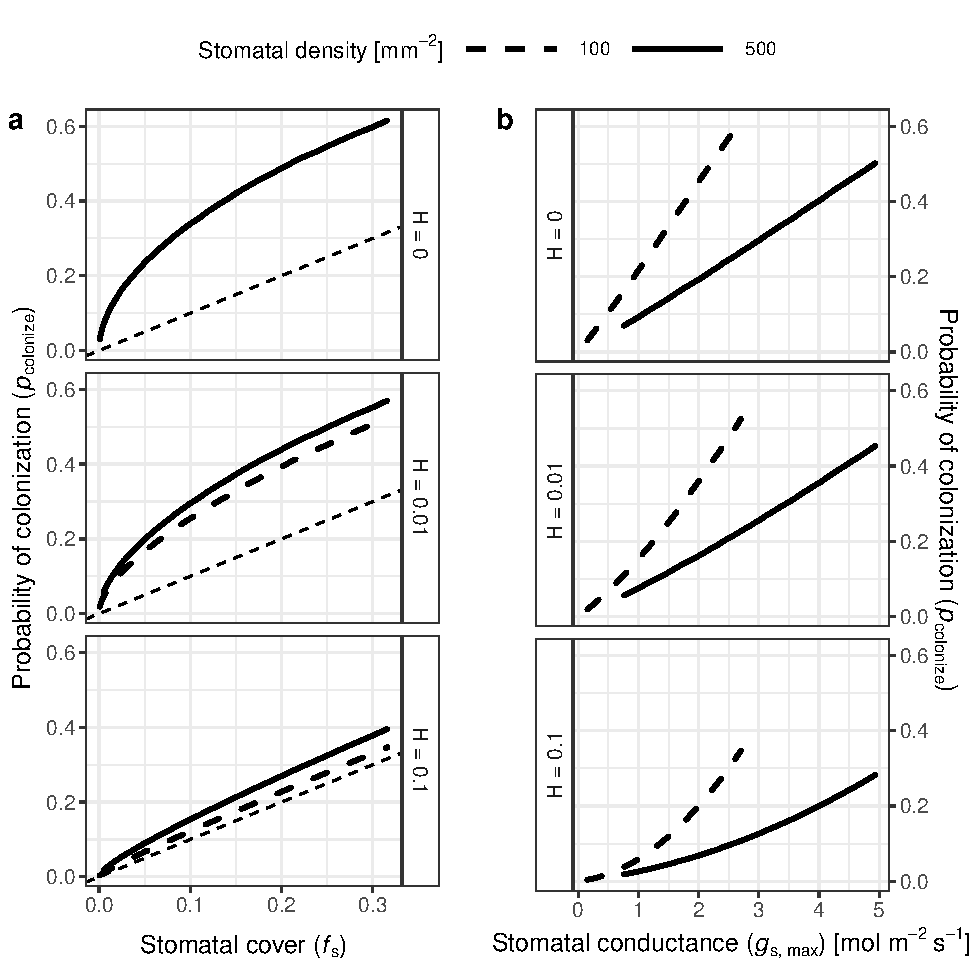
\includegraphics{../figures/fig3.pdf}
    \caption{\textbf{The probability of colonization increases with both stomatal cover and conductance} I simulated the probability of colonization ($p_\text{colonize}$, $y$-axis) over a range of stomatal densities and sizes (see [Materials and Methods]), but a subset of results are shown here. Stomatal size and density determine stomatal cover (\fs; Equation \ref{eq:fs}) and theoretical maximum stomatal conductance (\gsmax; Equation \ref{eq:gsmax}). \textbf{a.} $p_\text{colonize}$ initially increases rapidly with \fs{} ($x$-axis), then slows down to a linear relationship. Overall, $p_\text{colonize}$ is lower when pathogens can die on the leaf surface ($H > 0$). The relationship between \fs{} and $p_\text{colonize}$ is the same regardless of stomatal density when $H = 0$ (upper facet), which is why the lines overlap. When $H > 0$, higher density (solid lines) increase $p_\text{colonize}$ (lower facets). \textbf{b.} $p_\text{colonize}$ increases exponentially with \gsmax{} at all stomatal densities, but $p_\text{colonize}$ is much lower at higher densities for a given \gsmax. The relationship between \gsmax{} and $p_\text{colonize}$ is similar for all values of $H$.}
    \label{fig:fig3}
\end{figure}

\hypertarget{hyper-conductance-size-density-scaling}{%
\subsection*{Hyper-conductance size-density
scaling}\label{hyper-conductance-size-density-scaling}}
\addcontentsline{toc}{subsection}{Hyper-conductance size-density
scaling}

The scaling relationship between \(S\) and \(D\) that preserves
\(p_\text{colonize}\) is always greater than 0.5 (hyper-conductance),
but usually less than 1. When \(H = 0\), the scaling relationship is
essentially 1 (Figure \ref{fig:fig4}), which means that an increase
\fs{} leads to a proportional increase in \(p_\text{colonize}\). Because
the scaling relationship is greater than 0.5, leaves with greater
stomatal density will have lower \(p_\text{colonize}\) than leaves lower
stomatal density but the same \gsmax. In other words, increasing \(D\)
and lowering \(S\) allows plants to reduce \(p_\text{colonize}\) while
maintaining \gsmax. The scaling relationship is slightly less than 1,
but still greater than 0.5, when \(H > 0\) (Figure \ref{fig:fig4}). In
this area of parameter space, lower stomatal density can reduce \fs{}
while \(p_\text{colonize}\) is constant, but this will still result in
lower \gsmax. In the spatially implicit model, the size-density scaling
exponent was always exactly 1 except when \(H = 0\) (Appendix 1).

\begin{figure}
  \centering
    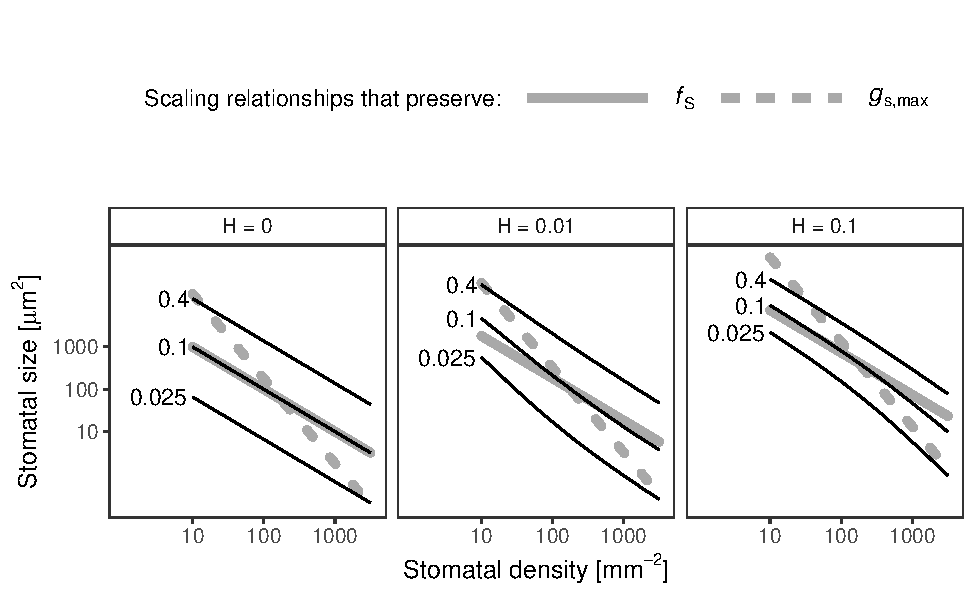
\includegraphics{../figures/fig4.pdf}
    \caption{\textbf{Log-log scaling relationships between stomatal density ($D$, \textit{x}-axis) and size ($S$, \textit{y}-axis) that preserve the probability of colonization ($p_\text{colonize}$).} In each panel, solid lines indicate values of $D$ and $S$ where $p_\text{colonize}$ is 0.025 (lowest line), 0.1, or 0.4 (highest line). For reference, dashed grey lines show scaling relationships that preserve \fs{} ($\beta = 1$, $\text{slope} = - 1 / \beta = -1$) and \gsmax{} ($\beta = 0.5$, $\text{slope} = - 1 / \beta = -2$) drawn through the centroid of the plotting region. When the death rate on the leaf surface is low ($H = 0$), the scaling exponent is very close to $\beta = 1$. When $H > 0$, $0.5 < \beta < 1$ and is slightly nonlinear on a log-log scale.}
    \label{fig:fig4}
\end{figure}

\hypertarget{discussion}{%
\section*{Discussion}\label{discussion}}
\addcontentsline{toc}{section}{Discussion}

Stomatal density and size set the upper limit on gas exchange in leaves
(Harrison et al., 2019) and is often closely related to operational
stomatal conductance in nature (Murray et al., 2019). Despite the fact
that many foliar pathogens infect through stomata, the relationship
between stomatal anatomy and resistance to foliar pathogens is less
clear than it is for gas exchange. I used a spatially explicit model of
a pathogen searching for a stomate to colonize a host. From this
\protect\hyperlink{model}{Model}, I derived predictions about the
relationship between stomatal anatomy and the probability of
colonization, a component of disease resistance. The model predicts that
the probability of colonization is not always proportional to the
surface area of leaf covered by stomata (\fs), as one might intuitively
predict. If the leaf surface is a hostile environment and pathogens have
a limited time to search, lower stomatal density decreases the
probability of colonization even if \fs{} is constant. However, \gsmax{}
decreases proportionally more than the probability of colonization. The
model highlights the potential for conflicting demands of minimizing
pathogen colonization, minimizing stomatal cover, and maintaining
stomatal conductance. Including the effect of anatomy on pathogen
colonization therefore has the potential to change our understanding of
how stomatal size-density scaling evolves in land plants.

The model predicts that in most cases, increasing stomatal cover should
lead to a proportional increase in colonization, which agrees with
empirical studies (e.g.~McKown et al. (2014); Tateda et al. (2019);
Dutton et al. (2019); Fetter et al. (2019)). It also makes new, testable
predictions that are less intuitive (Table 2). At very low \fs, there is
a rapid increase in colonization (Figure \ref{fig:fig3}a). If there are
no stomata, the probability of colonization is 0, so the first few
stomata dramatically increase the probability. This is less likely to be
significant for abaxial (lower) leaf surfaces, which usually have most
of the stomata (Salisbury, 1928; Metcalfe and Chalk, 1950; Mott et al.,
1984; Peat and Fitter, 1994; Jordan et al., 2014; Muir, 2015; Bucher et
al., 2017; Drake et al., 2019). However, many adaxial (upper) leaf
surfaces have zero or very few stomata. Using adaxial leaf surfaces, it
should be possible to test if small changes in stomatal size or density
have a larger effect on pathogen colonization when \fs{} is low. Such
experiments could use natural genetic variation (McKown et al., 2014) or
mutant lines (Dow et al., 2014b). The nonlinear increase in
\(p_\text{colonize}\) is less apparent when \(H > 0\) (Figure
\ref{fig:fig3}a). A more hostile microenvironment (e.g.~drier, higher
UV) should therefore reduce the effect of increased size or density at
low \fs. If true, the diminishing marginal effect of \fs{} on
colonization could explain why stomatal ratio on the upper and lower
surface is bimodal (Muir, 2015). The initial cost of adaxial (upper)
stomata is relatively high, but if the benefits outweigh the costs, then
equal stomatal densities on each surface maximize CO\(_2\) supply for
photosynthesis (Parkhurst, 1978; Gutschick, 1984; Parkhurst and Mott,
1990). The costs and benefits will certainly vary with environmental
conditions as well. Future work should extend this model, which
considered hypostomatous leaves, to address stomatal size and density in
amphistomatous leaves, since leaf surfaces may differ in the type of
pathogens present and microenvironment (McKown et al., 2014; Fetter et
al., 2019).

\textbf{Table 2} \textbar{} New testable model predictions and suggested
experiments to test them.

\begin{longtable}[]{@{}ll@{}}
\toprule
\begin{minipage}[b]{0.50\columnwidth}\raggedright
Model Prediction\strut
\end{minipage} & \begin{minipage}[b]{0.44\columnwidth}\raggedright
How to test it\strut
\end{minipage}\tabularnewline
\midrule
\endhead
\begin{minipage}[t]{0.50\columnwidth}\raggedright
Increasing stomatal size and/or density will have a larger effect on
pathogen colonization in leaves with low stomatal cover.\strut
\end{minipage} & \begin{minipage}[t]{0.44\columnwidth}\raggedright
Compare the effect of changing stomatal size and/or density on pathogen
colonization in leaves with low and high stomatal cover.\strut
\end{minipage}\tabularnewline
\begin{minipage}[t]{0.50\columnwidth}\raggedright
Increasing stomatal size and/or density will have a smaller effect on
pathogen colonization in ephiphytic environments more hostile to
pathogens.\strut
\end{minipage} & \begin{minipage}[t]{0.44\columnwidth}\raggedright
Compare the effect of changing stomatal size and/or density on pathogen
colonization in more hostile environments (e.g.~drier, higher
light)\strut
\end{minipage}\tabularnewline
\begin{minipage}[t]{0.50\columnwidth}\raggedright
When selection against pathogen colonization is stronger, the stomatal
size-density scaling exponent should be lower\strut
\end{minipage} & \begin{minipage}[t]{0.44\columnwidth}\raggedright
Measure stomatal anatomy in environments that differ in pathogen
colonization using comparative or experimental approaches\strut
\end{minipage}\tabularnewline
\bottomrule
\end{longtable}

An effect of stomatal size and density on foliar pathogen colonization
could change our understanding of stomatal size-density scaling. Since
allocating leaf epidermis to stomata may be costly (Franks and Farquhar,
2007; Assmann and Zeiger, 1987; Dow et al., 2014b; Lehmann and Or, 2015;
Baresch et al., 2019), selection should favor leaves that achieve a
desired \gsmax{} while minimizing \fs{} (Boer et al., 2016). Because of
their different scaling exponents (Equation \ref{eq:gsmax},
\ref{eq:fs}), smaller, densely packed stomata can achieve the same
\gsmax{} at minimum \fs. However, many leaves have larger, sparsely
packed stomata. Incorporating pathogen colonization may explain why. If
pathogens have a limited time to find stomata before dying (\(H > 0\)),
then the scaling exponent between size and density that keeps
\(p_\text{colonize}\) constant is between 0.5 and 1, the scaling
exponents for \gsmax{} and \fs, respectively (Figure \ref{fig:fig4}).
Greater density of smaller stomata can increase \gsmax{} while keeping
\(p_\text{colonize}\) constant, but this will increase \fs. Conversely,
\fs{} could decrease while keeping \(p_\text{colonize}\) constant, but
this will decrease \gsmax. This sets up the potential for conflict
between competing goals. The optimal stomatal size and density will
therefore depend on the precise costs and benefits of infection,
stomatal conductance, and stomatal cover. This may explain why many
leaves have large, sparsely packed stomata despite the fact that they
could achieve the same \gsmax{} and lower \fs{} with smaller, more
densely packed stomata.

The model examines the probability of colonization for a single
pathogen. The calculated probabilities of colonization should not be
interpreted as exact predictions, but rather as depicting qualitative
relationships between stomatal anatomy and infection severity. The
energetic cost and lost photosynthetic capacity (closed stomata,
necrosis, etc.) of dealing with a pathogen is assumed to be proportional
to the amount of infection. The actual fitness cost will be modulated by
the number of pathogens landing on the leaf and the cost of infection,
all else being equal. In environments with fewer or less virulent
pathogens, the fitness cost of infection will be less than in
environments with more abundant, virulent pathogens. The model is less
relevant to very susceptible host plants that can be severely damaged or
killed by a small number of colonizations that spread unchecked
throughout the host tissue.

\hypertarget{conclusion}{%
\section*{Conclusion}\label{conclusion}}
\addcontentsline{toc}{section}{Conclusion}

The model makes two non-intuitive predictions. First, the effect of
increased stomatal density or size on susceptibility to foliar pathogens
is greatest when stomatal cover is very low. Second, maximizing disease
resistance sets up a potential conflict between minimizing stomatal
cover and maximizing stomatal conductance. The first prediction is
consistent with results in \emph{Populus trichocarpa} (McKown et al.,
2014) and may be relatively straightforward to test experimentally with
adaxial (upper) stomata that occur at low and moderate densities within
the same or closely related species (Muir et al., 2014; Fetter et al.,
2019). The second prediction about size-density scaling is more complex
because we would need to know the relationships between colonization,
stomatal cover, stomatal conductance, and fitness in natural conditions.
There is growing evidence that stomata mediate tradeoffs between
photosynthesis and defense in \emph{Populus trichocarpa} (McKown et al.,
2019), but testing these predictions in a variety of species will help
determine whether pathogens have played an important role shaping
stomatal anatomy in land plants.

\hypertarget{acknowledgments}{%
\section*{Acknowledgments}\label{acknowledgments}}
\addcontentsline{toc}{section}{Acknowledgments}

I would like to thank Athena McKown and Karl Fetter for valuable
feedback that improved this manuscript.

\hypertarget{funding}{%
\section*{Funding}\label{funding}}
\addcontentsline{toc}{section}{Funding}

I am grateful startup funds from the University of Hawai'i for
supporting this work.

\hypertarget{conflict-of-interest-statement}{%
\section*{Conflict of Interest
Statement}\label{conflict-of-interest-statement}}
\addcontentsline{toc}{section}{Conflict of Interest Statement}

The author declares that the research was conducted in the absence of
any commercial or financial relationships that could be construed as a
potential conflict of interest.

\clearpage

\hypertarget{supplementary-material}{%
\section*{Supplementary Material}\label{supplementary-material}}
\addcontentsline{toc}{section}{Supplementary Material}

\renewcommand{\theequation}{S\arabic{equation}}
\renewcommand{\thefigure}{S\arabic{figure}}
\renewcommand{\thetable}{S\arabic{table}}

\setcounter{equation}{0}    
\setcounter{figure}{0}    
\setcounter{table}{0}

\hypertarget{g_textsmax-calculation}{%
\subsection*{\texorpdfstring{\(g_\text{s,max}\)
calculation}{g\_\textbackslash text\{s,max\} calculation}}\label{g_textsmax-calculation}}
\addcontentsline{toc}{subsection}{\(g_\text{s,max}\) calculation}

I calculated \gsmax{} (Equation \ref{eq:gsmax}) to water vapor at a
reference leaf temperature (\(T_\mathrm{leaf} = 25 ^ \circ\) C)
following Sack and Buckley (2016). They defined a biophysical and
morphological constant as:

\begin{align*}
  b = & D_\text{wv} / v \\
  m = & \frac{\pi c ^ 2}{j ^ {0.5} (4 h j + \pi c)}
\end{align*}

\(b\) is the diffusion coefficient of water vapor in air
(\(D_\text{wv}\)) divided by the kinematic viscosity of dry air (\(v\)).
\(D_\text{wv} = 2.49 \times 10^{-5} ~ \text{m}^2 ~ \text{s}^{-1}\) and
\(v = 2.24 \times 10 ^ {-2} ~ \text{m}^3 ~ \text{mol} ^ {-1}\) at
\(25 ^ \circ\) (Monteith and Unsworth, 2013). For kidney-shaped guard
cells, \(c = h = j = 0.5\).

\hypertarget{is-proportional-to-the-stomatal-pore-area-index}{%
\subsection*{\texorpdfstring{\fs{} is proportional to the stomatal pore
area
index}{ is proportional to the stomatal pore area index}}\label{is-proportional-to-the-stomatal-pore-area-index}}
\addcontentsline{toc}{subsection}{\fs{} is proportional to the stomatal
pore area index}

The stomatal pore area index (SPI; Sack et al., 2003) is calculated as
the product of the stomatal density and guard cell length (GCL) squared:

\begin{equation*}
  \mathrm{SPI} = D \times \mathrm{GCL} ^ 2
\end{equation*}

Assuming that the stomatal radius \(R\) is half the GCL, then stomatal
size \(S\) is equivalent to:

\begin{equation*}
  S = \pi R ^ 2 = \frac{\pi \times \mathrm{GCL} ^ 2}{4}
\end{equation*}

Based on equation \ref{eq:fs}, it follows that \fs{} and SPI are
proportional:

\begin{equation*}
  f_\text{S} = \frac{\pi \times \mathrm{SPI}}{4}
\end{equation*}

\clearpage

\hypertarget{appendix-1-spatially-implicit-model}{%
\section*{Appendix 1: Spatially implicit
model}\label{appendix-1-spatially-implicit-model}}
\addcontentsline{toc}{section}{Appendix 1: Spatially implicit model}

A limitation of the spatially explicit model is that a pathogen could
only infect stomata in the focal triangle where it landed. Here I
analyze an alternative, spatially implicit, model that relaxes this
assumptions. Instead, I assume that a pathogen can potentially infect
any stomate on the leaf. It searches through a random walk and has a
continuous, constant probability of encountering a stomate that is
determined by stomatal cover (\fs). If \(fs << 1\), this can be modeled
as a homogeneous Poisson process and the distance \(x\) a pathogen must
travel before reaching a stomate follows an exponential distribution:

\begin{equation*}
  f(x) = f_\text{S} e ^ {-f_\text{S} x}
\end{equation*}

Given the constant death rate per unit distance \(H\), the probability
of surviving to distance \(x\) is \(e^{-H x}\). The probability of
locating a stomate the probability of surviving to distance \(x\)
multiplied by \(f(x)\) and integrated over all \(x\) from 0 to
\(\infty\):

\begin{align*}
  p_\text{locate} & = \int_0^\infty f(x) e^{-Hx} dx \\
                  & = \int_0^\infty f_\text{S} e^{-(f_\text{S} + H)x} dx \\
                  & = \frac{f_\text{S}}{H + f_\text{S}}
\end{align*}

Substituting \(p_\text{locate}\) above into Equation
\ref{eq:p_colonize}:

\begin{align*}
  p_\text{colonize} & = f_\text{S} + (1 - f_\text{S}) p_\text{locate} \\
                    & = f_\text{S} + (1 - f_\text{S}) \frac{f_\text{S}}{H + f_\text{S}} \\
                    & = f_\text{S} (1 + \frac{1 - f_\text{S}}{H + f_\text{S}})
\end{align*}

With the spatially implicit model, because pathogens can potentially
reach any stomate on the leaf, \(p_\text{colonize}\) is greater than
that in the spatially explicit model for the same value of \(H\). For
example, if the pathogen can search forever (\(H = 0\)), then it will
always colonize (\(p_\text{colonize} = 1\); Figure \ref{fig:figS2}a).
But even when \(H > 0\), \(p_\text{colonize}\) is significantly higher
than in the spatially implicit than spatially explicit model for the
same \fs{} because pathogens can potentially colonize any stomate on the
leaf.

Whereas the spatially explicit model probably underestimates
\(p_\text{locate}\) for pathogens that can search over long distances,
the implicit model overestimates because it assumes that the probability
of encountering a stomate is constant (i.e.~homogeneous Poisson
process). This is not true because stomata are discrete areas on the
leaf. If a pathogen is searching far away from a stomate, its
probability of encountering a stomate in the near future is lower than
that for a pathogen searching near a stomate. This should be modeled as
a \emph{nonhomogenous} Poisson process. Future work should derive
\(p_\text{locate}\) for the stomatal anatomies presented here under a
nonhomogeneous process.

Despite the quantitative differences in the the spatially explicit and
implicit models, they have similar qualitative properties when
\(H > 0\), which is reasonable since the leaf surface is a relatively
hostile environment for most pathogens (see
\protect\hyperlink{introduction}{Introduction}). In both models,
\(p_\text{colonize}\) increases with, but is higher than \fs. In the
spatially explicit model, size-density scaling that preserves
\(p_\text{colonize}\) is 1 when \(H = 0\) and slightly less than 1
otherwise (Figure \ref{fig:fig4}). In the spatially implicit model, the
scaling coefficient is always 1. Rearranging the equation for
\(p_\text{colonize}\) above and substituting \(f_\text{S} = DS\), the
following relationship holds:

\[SD = \frac{p_\text{colonize} H}{1 - p_\text{colonize} + H}\] Since
\(H\) is a constant the right-hand side of the equation above is
constant for a given value of \(p_\text{colonize}\). Hence the
\(\beta_p\) that would preserve the relationship above is simply 1
(Figure \ref{fig:figS3}).

\hypertarget{figures}{%
\subsection*{Figures}\label{figures}}
\addcontentsline{toc}{subsection}{Figures}

\begin{figure}
  \centering
    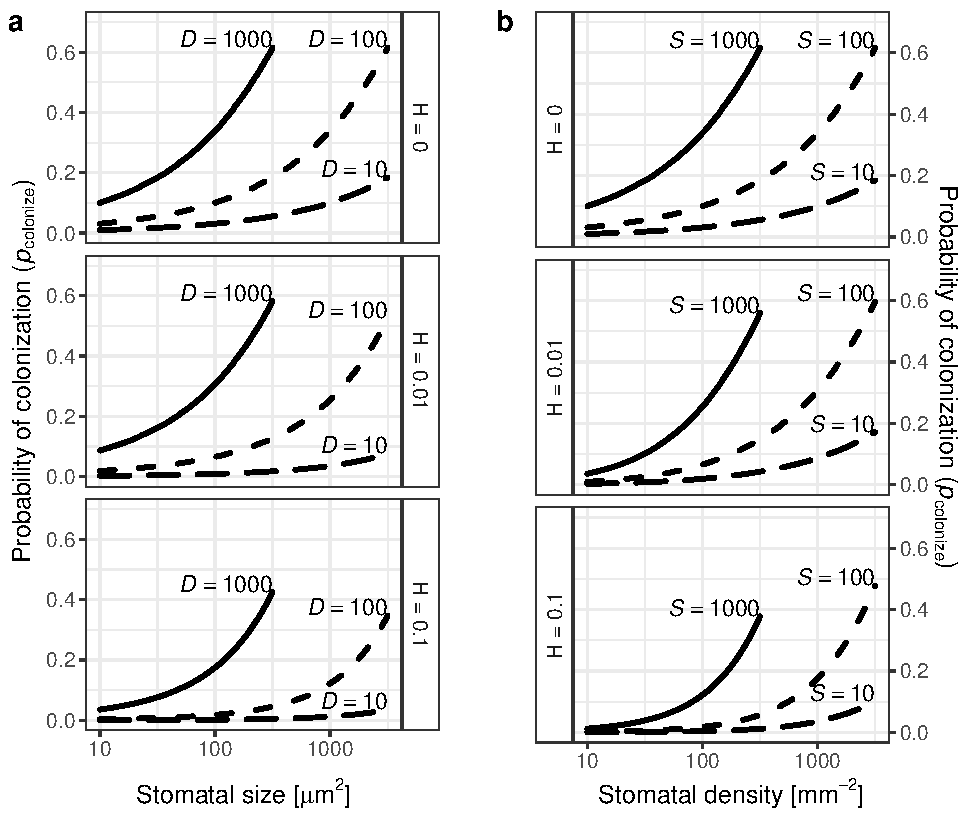
\includegraphics{../figures/figS1.pdf}
    \caption{\textbf{The probability of colonization increases with both stomatal size ($S$) and density $D$} I simulated the probability of colonization ($p_\text{colonize}$, $y$-axis) over a range of $S$, $D$, and $H$ (see [Materials and Methods]) \textbf{a.} Each line shows how $p_\text{colonize}$ increases with $S$ ($x$-axis, log-scale) for selected values of $D \in \{10, 100, 1000\}~\text{mm}^{-2}$. \textbf{b.} Each line shows how $p_\text{colonize}$ increases with $D$ ($x$-axis, log-scale) for selected values of $S \in \{10, 100, 1000\}~\mu\text{m}^2$. The facets show results for different values of $H$}
    \label{fig:figS1}
\end{figure}

\begin{figure}
  \centering
    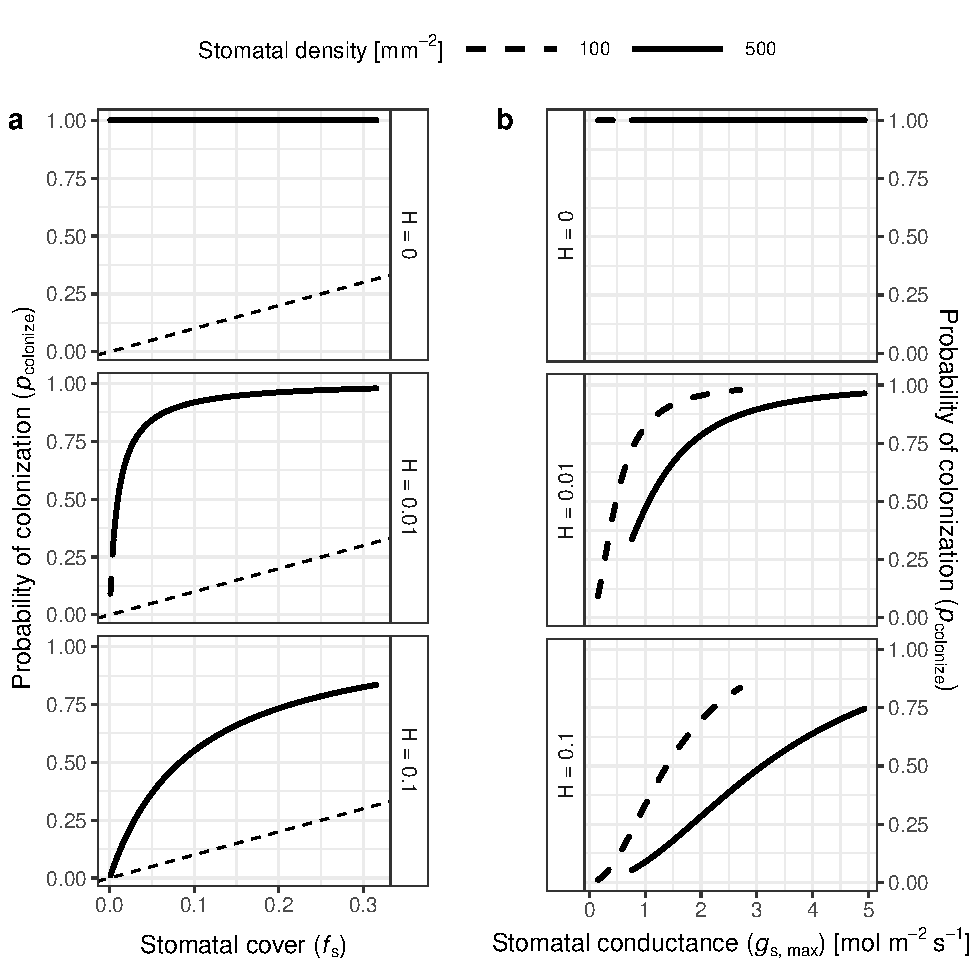
\includegraphics{../figures/figS2.pdf}
    \caption{\textbf{The probability of colonization increases with both stomatal cover and conductance in the spatially implicit model.} As in Figure \ref{fig:fig3}, I simulated the probability of colonization ($p_\text{colonize}$, $y$-axis) over a range of stomatal densities and sizes (see [Materials and Methods]), but a subset of results are shown here. Stomatal size and density determine stomatal cover (\fs; Equation \ref{eq:fs}) and theoretical maximum stomatal conductance (\gsmax; Equation \ref{eq:gsmax}). \textbf{a.} $p_\text{colonize}$ initially increases rapidly with \fs{} ($x$-axis), then slows down to a linear relationship. Overall, $p_\text{colonize}$ is lower when pathogens can die on the leaf surface ($H > 0$). The relationship between \fs{} and $p_\text{colonize}$ is the same regardless of stomatal density for all values of $H$, which is why the lines overlap. \textbf{b.} $p_\text{colonize}$ increases sigmoidally with \gsmax{} at all stomatal densities, but $p_\text{colonize}$ is lower at higher densities for a given \gsmax. The relationship between \gsmax{} and $p_\text{colonize}$ is similar for all values of $H > 0$.}
    \label{fig:figS2}
\end{figure}

\begin{figure}
  \centering
    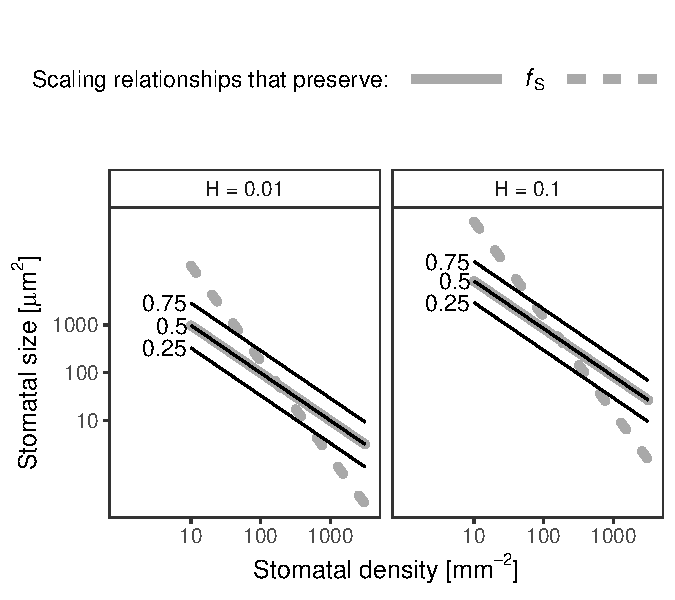
\includegraphics{../figures/figS3.pdf}
    \caption{\textbf{Log-log scaling relationships between stomatal density ($D$, \textit{x}-axis) and size ($S$, \textit{y}-axis) that preserve the probability of colonization ($p_\text{colonize}$) in the spatially implicit model}. As in Figure \ref{fig:fig4}, in each panel, solid lines indicate values of $D$ and $S$ where $p_\text{colonize}$ is 0.25 (lowest line), 0.5, or 0.75 (highest line). For reference, dashed grey lines show scaling relationships that preserve \fs{} ($\beta = 1$, $\text{slope} = - 1 / \beta = -1$) and \gsmax{} ($\beta = 0.5$, $\text{slope} = - 1 / \beta = -2$) drawn through the centroid of the plotting region. The scaling exponent is unity $\beta = 1$ when $H > 0$.}
    \label{fig:figS3}
\end{figure}

\clearpage

\hypertarget{references}{%
\section*{References}\label{references}}
\addcontentsline{toc}{section}{References}

\hypertarget{refs}{}
\begin{cslreferences}
\leavevmode\hypertarget{ref-allaire_rmarkdown:_2020}{}%
Allaire, J., Xie, Y., McPherson, J., Luraschi, J., Ushey, K., Wickham,
H., Cheng, J., Chang, W., and Iannone, R. (2020). Rmarkdown: Dynamic
Documents for R. Available at:
\url{https://github.com/rstudio/rmarkdown}.

\leavevmode\hypertarget{ref-allen_appressorium_1991}{}%
Allen, E. A., Hazen, B. E., Hoch, H. C., Kwon, Y., Leinhos, G. M. E.,
Staples, R. C., Stumpf, M. A., and Terhune, B. T. (1991). Appressorium
Formation in Response to Topographical Signals by 27 Rust Species.
\emph{Phytopathology} 81, 323.
doi:\href{https://doi.org/10.1094/Phyto-81-323}{10.1094/Phyto-81-323}.

\leavevmode\hypertarget{ref-assmann_guard_1987}{}%
Assmann, S. M., and Zeiger, E. (1987). ``Guard Call Bioenergetics,'' in
\emph{Stomatal Function}, eds. E. Zeiger, G. D. Farquhar, and I. R.
Cowan (Stanford University Press), 163--193.

\leavevmode\hypertarget{ref-baresch_competition_2019}{}%
Baresch, A., Crifò, C., and Boyce, C. K. (2019). Competition for
epidermal space in the evolution of leaves with high physiological
rates. \emph{New Phytologist} 221, 628--639.
doi:\href{https://doi.org/10.1111/nph.15476}{10.1111/nph.15476}.

\leavevmode\hypertarget{ref-bastiaans_ratio_1991}{}%
Bastiaans, L. (1991). Ratio Between Virtual and Visual Lesion Size as a
Measure to Describe Reduction in Leaf Photosynthesis of Rice Due to Leaf
Blast. \emph{Phytopathology} 81, 611.
doi:\href{https://doi.org/10.1094/Phyto-81-611}{10.1094/Phyto-81-611}.

\leavevmode\hypertarget{ref-beattie_secret_1995}{}%
Beattie, G. A., and Lindow, S. E. (1995). The secret life of foliar
bacterial pathogens on leaves. \emph{Annual Review of Phytopathology}
33, 145--172.

\leavevmode\hypertarget{ref-berry_stomata:_2010}{}%
Berry, J. A., Beerling, D. J., and Franks, P. J. (2010). Stomata: Key
players in the earth system, past and present. \emph{Current Opinion in
Plant Biology} 13, 232--239.
doi:\href{https://doi.org/10.1016/j.pbi.2010.04.013}{10.1016/j.pbi.2010.04.013}.

\leavevmode\hypertarget{ref-de_boer_optimal_2016}{}%
Boer, H. J. de, Price, C. A., Wagner-Cremer, F., Dekker, S. C., Franks,
P. J., and Veneklaas, E. J. (2016). Optimal allocation of leaf epidermal
area for gas exchange. \emph{New Phytologist} 210, 1219--1228.
doi:\href{https://doi.org/10.1111/nph.13929}{10.1111/nph.13929}.

\leavevmode\hypertarget{ref-borchers_pracma:_2019}{}%
Borchers, H. W. (2019). Pracma: Practical Numerical Math Functions. R
package version 2.2.9. Available at:
\url{https://CRAN.R-project.org/package=pracma}.

\leavevmode\hypertarget{ref-perez-martin_tropic_2012}{}%
Brand, A., and Gow, N. A. R. (2012). ``Tropic Orientation Responses of
Pathogenic Fungi,'' in \emph{Morphogenesis and Pathogenicity in Fungi},
eds. J. Pérez-Martín and A. Di Pietro (Berlin, Heidelberg: Springer
Berlin Heidelberg), 21--41.
doi:\href{https://doi.org/10.1007/978-3-642-22916-9_2}{10.1007/978-3-642-22916-9\_2}.

\leavevmode\hypertarget{ref-brodribb_unified_2013}{}%
Brodribb, T. J., Jordan, G. J., and Carpenter, R. J. (2013). Unified
changes in cell size permit coordinated leaf evolution. \emph{New
Phytologist} 199, 559--570.
doi:\href{https://doi.org/10.1111/nph.12300}{10.1111/nph.12300}.

\leavevmode\hypertarget{ref-brown_static_1900}{}%
Brown, H. T., and Escombe, F. (1900). Static diffusion of gases and
liquids in relation to the assimilation of carbon and translocation in
plants. \emph{Proceedings of the Royal Society of London} 67, 124--128.

\leavevmode\hypertarget{ref-bucher_stomatal_2017}{}%
Bucher, S. F., Auerswald, K., Grün-Wenzel, C., Higgins, S. I., Garcia
Jorge, J., and Römermann, C. (2017). Stomatal traits relate to habitat
preferences of herbaceous species in a temperate climate. \emph{Flora}
229, 107--115.
doi:\href{https://doi.org/10.1016/j.flora.2017.02.011}{10.1016/j.flora.2017.02.011}.

\leavevmode\hypertarget{ref-buckley_how_2019}{}%
Buckley, T. N. (2019). How do stomata respond to water status? \emph{New
Phytologist} 224, 21--36.
doi:\href{https://doi.org/10.1111/nph.15899}{10.1111/nph.15899}.

\leavevmode\hypertarget{ref-chater_origins_2017}{}%
Chater, C. C. C., Caine, R. S., Fleming, A. J., and Gray, J. E. (2017).
Origins and Evolution of Stomatal Development. \emph{Plant Physiology}
174, 624--638.
doi:\href{https://doi.org/10.1104/pp.17.00183}{10.1104/pp.17.00183}.

\leavevmode\hypertarget{ref-dow_integrated_2014}{}%
Dow, G. J., Bergmann, D. C., and Berry, J. A. (2014a). An integrated
model of stomatal development and leaf physiology. \emph{New
Phytologist} 201, 1218--1226.

\leavevmode\hypertarget{ref-dow_physiological_2014}{}%
Dow, G. J., Berry, J. A., and Bergmann, D. C. (2014b). The physiological
importance of developmental mechanisms that enforce proper stomatal
spacing in \emph{Arabidopsis thaliana}. \emph{New Phytologist} 201,
1205--1217.
doi:\href{https://doi.org/10.1111/nph.12586}{10.1111/nph.12586}.

\leavevmode\hypertarget{ref-drake_two_2019}{}%
Drake, P. L., Boer, H. J., Schymanski, S. J., and Veneklaas, E. J.
(2019). Two sides to every leaf: Water and \textless span
style="font-variant:Small-caps;"\textgreater CO\textless/span\textgreater{}
\(_{\textrm{2}}\) transport in hypostomatous and amphistomatous leaves.
\emph{New Phytologist} 222, 1179--1187.
doi:\href{https://doi.org/10.1111/nph.15652}{10.1111/nph.15652}.

\leavevmode\hypertarget{ref-drake_smaller_2013}{}%
Drake, P. L., Froend, R. H., and Franks, P. J. (2013). Smaller, faster
stomata: Scaling of stomatal size, rate of response, and stomatal
conductance. \emph{Journal of Experimental Botany} 64, 495--505.
doi:\href{https://doi.org/10.1093/jxb/ers347}{10.1093/jxb/ers347}.

\leavevmode\hypertarget{ref-dutton_bacterial_2019}{}%
Dutton, C., Hõrak, H., Hepworth, C., Mitchell, A., Ton, J., Hunt, L.,
and Gray, J. E. (2019). Bacterial infection systemically suppresses
stomatal density. \emph{Plant, Cell \& Environment} 42, 2411--2421.
doi:\href{https://doi.org/10.1111/pce.13570}{10.1111/pce.13570}.

\leavevmode\hypertarget{ref-farquhar_stomatal_1982}{}%
Farquhar, G. D., and Sharkey, T. D. (1982). Stomatal Conductance and
Photosynthesis. \emph{Annual Review of Plant Physiology} 33, 317--345.
doi:\href{https://doi.org/10.1146/annurev.pp.33.060182.001533}{10.1146/annurev.pp.33.060182.001533}.

\leavevmode\hypertarget{ref-fawke_oomycete_2015}{}%
Fawke, S., Doumane, M., and Schornack, S. (2015). Oomycete Interactions
with Plants: Infection Strategies and Resistance Principles.
\emph{Microbiology and Molecular Biology Reviews} 79, 263--280.
doi:\href{https://doi.org/10.1128/MMBR.00010-15}{10.1128/MMBR.00010-15}.

\leavevmode\hypertarget{ref-fetter_trade-offs_2019}{}%
Fetter, K. C., Nelson, D. M., and Keller, S. R. (2019). Trade-offs and
selection conflicts in hybrid poplars indicate the stomatal ratio as an
important trait regulating disease resistance. University of Vermont
doi:\href{https://doi.org/10.1101/814046}{10.1101/814046}.

\leavevmode\hypertarget{ref-flexas_co2_2018}{}%
Flexas, J., Cano, F. J., Carriquí, M., Coopman, R. E., Mizokami, Y.,
Tholen, D., and Xiong, D. (2018). ``CO2 Diffusion Inside Photosynthetic
Organs,'' in \emph{The Leaf: A Platform for Performing Photosynthesis}
Advances in Photosynthesis and Respiration., eds. W. W. Adams III and I.
Terashima (Cham: Springer International Publishing), 163--208.
doi:\href{https://doi.org/10.1007/978-3-319-93594-2_7}{10.1007/978-3-319-93594-2\_7}.

\leavevmode\hypertarget{ref-franks_co_2009}{}%
Franks, P. J., and Beerling, D. J. (2009a). CO \(_{\textrm{2}}\) -forced
evolution of plant gas exchange capacity and water-use efficiency over
the Phanerozoic. \emph{Geobiology} 7, 227--236.
doi:\href{https://doi.org/10.1111/j.1472-4669.2009.00193.x}{10.1111/j.1472-4669.2009.00193.x}.

\leavevmode\hypertarget{ref-franks_maximum_2009}{}%
Franks, P. J., and Beerling, D. J. (2009b). Maximum leaf conductance
driven by CO\(_{\textrm{2}}\) effects on stomatal size and density over
geologic time. \emph{Proceedings of the National Academy of Sciences}
106, 10343--10347.

\leavevmode\hypertarget{ref-franks_plasticity_2009}{}%
Franks, P. J., Drake, P. L., and Beerling, D. J. (2009). Plasticity in
maximum stomatal conductance constrained by negative correlation between
stomatal size and density: An analysis using \emph{Eucalyptus globulus}.
\emph{Plant, Cell \& Environment} 32, 1737--1748.
doi:\href{https://doi.org/10.1111/j.1365-3040.2009.002031.x}{10.1111/j.1365-3040.2009.002031.x}.

\leavevmode\hypertarget{ref-franks_effect_2001}{}%
Franks, P. J., and Farquhar, G. D. (2001). The effect of exogenous
abscisic acid on stomatal development, stomatal mechanics, and leaf gas
exchange in \emph{Tradescantia virginiana}. \emph{Plant Physiology} 125,
935--942.

\leavevmode\hypertarget{ref-franks_mechanical_2007}{}%
Franks, P. J., and Farquhar, G. D. (2007). The Mechanical Diversity of
Stomata and Its Significance in Gas-Exchange Control. \emph{Plant
Physiology} 143, 78--87.
doi:\href{https://doi.org/10.1104/pp.106.089367}{10.1104/pp.106.089367}.

\leavevmode\hypertarget{ref-franks_new_2014}{}%
Franks, P. J., Royer, D. L., Beerling, D. J., Van de Water, P. K.,
Cantrill, D. J., Barbour, M. M., and Berry, J. A. (2014). New
constraints on atmospheric CO \(_{\textrm{2}}\) concentration for the
Phanerozoic: Franks et al.: New constraints on Phanerozoic CO2.
\emph{Geophysical Research Letters} 41, 4685--4694.
doi:\href{https://doi.org/10.1002/2014GL060457}{10.1002/2014GL060457}.

\leavevmode\hypertarget{ref-gilbert_evolutionary_2002}{}%
Gilbert, G. S. (2002). Evolutionary Ecology of Plant Diseases in Natural
Ecosystems. \emph{Annual Review of Phytopathology} 40, 13--43.
doi:\href{https://doi.org/10.1146/annurev.phyto.40.021202.110417}{10.1146/annurev.phyto.40.021202.110417}.

\leavevmode\hypertarget{ref-gray_flanking_2020}{}%
Gray, A., Liu, L., and Facette, M. (2020). Flanking Support: How
Subsidiary Cells Contribute to Stomatal Form and Function.
\emph{Frontiers in Plant Science} 11.
doi:\href{https://doi.org/10.3389/fpls.2020.00881}{10.3389/fpls.2020.00881}.

\leavevmode\hypertarget{ref-gutschick_photosynthesis_1984}{}%
Gutschick, V. P. (1984). Photosynthesis model for C\(_{\textrm{3}}\)
leaves incorporating CO\(_{\textrm{2}}\) transport, propagation of
radiation, and biochemistry 1. Kinetics and their parameterization.
\emph{Photosynthetica} 18, 549--568.

\leavevmode\hypertarget{ref-harrison_influence_2019}{}%
Harrison, E. L., Arce Cubas, L., Gray, J. E., and Hepworth, C. (2019).
The influence of stomatal morphology and distribution on photosynthetic
gas exchange. \emph{The Plant Journal}, tpj.14560.
doi:\href{https://doi.org/10.1111/tpj.14560}{10.1111/tpj.14560}.

\leavevmode\hypertarget{ref-hetherington_role_2003}{}%
Hetherington, A. M., and Woodward, F. I. (2003). The role of stomata in
sensing and driving environmental change. \emph{Nature} 424, 901--908.
doi:\href{https://doi.org/10.1038/nature01843}{10.1038/nature01843}.

\leavevmode\hypertarget{ref-hoch_signaling_1987}{}%
Hoch, H. C., Staples, R. C., Whitehead, B., Comeau, J., and Wolf, E. D.
(1987). Signaling for Growth Orientation and Cell Differentiation by
Surface Topography in Uromyces. \emph{Science, New Series} 235,
1659--1662. Available at: \url{http://www.jstor.org/stable/1698314}.

\leavevmode\hypertarget{ref-jones_partitioning_1985}{}%
Jones, H. G. (1985). Partitioning stomatal and non-stomatal limitations
to photosynthesis. \emph{Plant, Cell \& Environment} 8, 95--104.
doi:\href{https://doi.org/10.1111/j.1365-3040.1985.tb01227.x}{10.1111/j.1365-3040.1985.tb01227.x}.

\leavevmode\hypertarget{ref-jordan_using_2014}{}%
Jordan, G. J., Carpenter, R. J., and Brodribb, T. J. (2014). Using
fossil leaves as evidence for open vegetation. \emph{Palaeogeography,
Palaeoclimatology, Palaeoecology} 395, 168--175.
doi:\href{https://doi.org/10.1016/j.palaeo.2013.12.035}{10.1016/j.palaeo.2013.12.035}.

\leavevmode\hypertarget{ref-kiefer_host_2002}{}%
Kiefer, B., Riemann, M., Büche, C., Kassemeyer, H.-H., and Nick, P.
(2002). The host guides morphogenesis and stomatal targeting in the
grapevine pathogen Plasmopara viticola. \emph{Planta} 215, 387--393.
doi:\href{https://doi.org/10.1007/s00425-002-0760-2}{10.1007/s00425-002-0760-2}.

\leavevmode\hypertarget{ref-lawson_stomatal_2014}{}%
Lawson, T., and Blatt, M. R. (2014). Stomatal Size, Speed, and
Responsiveness Impact on Photosynthesis and Water Use Efficiency.
\emph{Plant Physiology} 164, 1556--1570.
doi:\href{https://doi.org/10.1104/pp.114.237107}{10.1104/pp.114.237107}.

\leavevmode\hypertarget{ref-lawson_coordination_2018}{}%
Lawson, T., Terashima, I., Fujita, T., and Wang, Y. (2018).
``Coordination Between Photosynthesis and Stomatal Behavior,'' in
\emph{The Leaf: A Platform for Performing Photosynthesis} Advances in
Photosynthesis and Respiration., eds. W. W. Adams III and I. Terashima
(Cham: Springer International Publishing), 141--161.
doi:\href{https://doi.org/10.1007/978-3-319-93594-2_6}{10.1007/978-3-319-93594-2\_6}.

\leavevmode\hypertarget{ref-lehmann_effects_2015}{}%
Lehmann, P., and Or, D. (2015). Effects of stomata clustering on leaf
gas exchange. \emph{New Phytologist} 207, 1015--1025.
doi:\href{https://doi.org/10.1111/nph.13442}{10.1111/nph.13442}.

\leavevmode\hypertarget{ref-mcelwain_using_2016}{}%
McElwain, J. C., Yiotis, C., and Lawson, T. (2016). Using modern plant
trait relationships between observed and theoretical maximum stomatal
conductance and vein density to examine patterns of plant
macroevolution. \emph{New Phytologist} 209, 94--103.
doi:\href{https://doi.org/10.1111/nph.13579}{10.1111/nph.13579}.

\leavevmode\hypertarget{ref-mckown_association_2014}{}%
McKown, A. D., Guy, R. D., Quamme, L., Klápště, J., La Mantia, J.,
Constabel, C. P., El-Kassaby, Y. A., Hamelin, R. C., Zifkin, M., and
Azam, M. S. (2014). Association genetics, geography and ecophysiology
link stomatal patterning in \emph{Populus trichocarpa} with carbon gain
and disease resistance trade-offs. \emph{Molecular Ecology} 23,
5771--5790.
doi:\href{https://doi.org/10.1111/mec.12969}{10.1111/mec.12969}.

\leavevmode\hypertarget{ref-mckown_role_2019}{}%
McKown, A. D., Klápště, J., Guy, R. D., Corea, O. R. A., Fritsche, S.,
Ehlting, J., El‐Kassaby, Y. A., and Mansfield, S. D. (2019). A role for
\emph{speechless} in the integration of leaf stomatal patterning with
the growth vs disease trade‐off in poplar. \emph{New Phytologist},
nph.15911.
doi:\href{https://doi.org/10.1111/nph.15911}{10.1111/nph.15911}.

\leavevmode\hypertarget{ref-mclachlan_gate_2014}{}%
McLachlan, D. H., Kopischke, M., and Robatzek, S. (2014). Gate control:
Guard cell regulation by microbial stress. \emph{New Phytologist} 203,
1049--1063.
doi:\href{https://doi.org/10.1111/nph.12916}{10.1111/nph.12916}.

\leavevmode\hypertarget{ref-melotto_plant_2006}{}%
Melotto, M., Underwood, W., Koczan, J., Nomura, K., and He, S. Y.
(2006). Plant Stomata Function in Innate Immunity against Bacterial
Invasion. \emph{Cell} 126, 969--980.
doi:\href{https://doi.org/10.1016/j.cell.2006.06.054}{10.1016/j.cell.2006.06.054}.

\leavevmode\hypertarget{ref-melotto_stomatal_2017}{}%
Melotto, M., Zhang, L., Oblessuc, P. R., and He, S. Y. (2017). Stomatal
Defense a Decade Later. \emph{Plant Physiology} 174, 561--571.
doi:\href{https://doi.org/10.1104/pp.16.01853}{10.1104/pp.16.01853}.

\leavevmode\hypertarget{ref-metcalfe_anatomy_1950}{}%
Metcalfe, C. R., and Chalk, L. (1950). \emph{Anatomy of the
dicotyledons, Vols. 1 \& 2}. First. Oxford: Oxford University Press.

\leavevmode\hypertarget{ref-meurer_sympy:_2017}{}%
Meurer, A., Smith, C. P., Paprocki, M., Čertík, O., Kirpichev, S. B.,
Rocklin, M., Kumar, A., Ivanov, S., Moore, J. K., Singh, S., et al.
(2017). SymPy: Symbolic computing in Python. \emph{PeerJ Computer
Science} 3, e103.
doi:\href{https://doi.org/10.7717/peerj-cs.103}{10.7717/peerj-cs.103}.

\leavevmode\hypertarget{ref-mitchell_trophic_2003}{}%
Mitchell, C. E. (2003). Trophic control of grassland production and
biomass by pathogens. \emph{Ecology Letters} 6, 147--155.
doi:\href{https://doi.org/10.1046/j.1461-0248.2003.00408.x}{10.1046/j.1461-0248.2003.00408.x}.

\leavevmode\hypertarget{ref-monteith_principles_2013}{}%
Monteith, J. L., and Unsworth, M. H. (2013). \emph{Principles of
environmental physics: Plants, animals, and the atmosphere}. 4th ed.
Amsterdam ; Boston: Elsevier/Academic Press.

\leavevmode\hypertarget{ref-morison_lateral_2005}{}%
Morison, J. I. L., Emily Gallouët, Lawson, T., Cornic, G., Herbin, R.,
and work(s): N. R. B. R. (2005). Lateral Diffusion of CO\$\_2\$ in
Leaves Is Not Sufficient to Support Photosynthesis. \emph{Plant
Physiology} 139, 254--266. Available at:
\url{http://www.jstor.org/stable/4281859}.

\leavevmode\hypertarget{ref-mott_adaptive_1984}{}%
Mott, K. A., Gibson, A. C., and O'Leary, J. W. (1984). The adaptive
significance of amphistomatic leaves. \emph{Plant, Cell \& Environment}
5, 455--460.

\leavevmode\hypertarget{ref-muir_making_2015}{}%
Muir, C. D. (2015). Making pore choices: Repeated regime shifts in
stomatal ratio. \emph{Proceedings of the Royal Society B: Biological
Sciences} 282, 20151498.
doi:\href{https://doi.org/10.1098/rspb.2015.1498}{10.1098/rspb.2015.1498}.

\leavevmode\hypertarget{ref-muir_morphological_2014}{}%
Muir, C. D., Hangarter, R. P., Moyle, L. C., and Davis, P. A. (2014).
Morphological and anatomical determinants of mesophyll conductance in
wild relatives of tomato ( \emph{solanum} sect. \emph{Lycopersicon} ,
sect. \emph{Lycopersicoides} ; Solanaceae). \emph{Plant, Cell \&
Environment} 37, 1415--1426.
doi:\href{https://doi.org/10.1111/pce.12245}{10.1111/pce.12245}.

\leavevmode\hypertarget{ref-murray_consistent_2019}{}%
Murray, M., Soh, W. K., Yiotis, C., Spicer, R. A., Lawson, T., and
McElwain, J. C. (2019). Consistent relationship between field-measured
stomatal conductance and theoretical maximum stomatal conductance in
C\(_{\textrm{3}}\) woody angiosperms in four major biomes.
\emph{International Journal of Plant Sciences}, 706260.
doi:\href{https://doi.org/10.1086/706260}{10.1086/706260}.

\leavevmode\hypertarget{ref-murray_plant_2016}{}%
Murray, R. R., Emblow, M. S. M., Hetherington, A. M., and Foster, G. D.
(2016). Plant virus infections control stomatal development.
\emph{Scientific Reports} 6, 34507.
doi:\href{https://doi.org/10.1038/srep34507}{10.1038/srep34507}.

\leavevmode\hypertarget{ref-oguchi_leaf_2018}{}%
Oguchi, R., Onoda, Y., Terashima, I., and Tholen, D. (2018). ``Leaf
Anatomy and Function,'' in \emph{The Leaf: A Platform for Performing
Photosynthesis} Advances in Photosynthesis and Respiration., eds. W. W.
Adams III and I. Terashima (Cham: Springer International Publishing),
97--139.
doi:\href{https://doi.org/10.1007/978-3-319-93594-2_5}{10.1007/978-3-319-93594-2\_5}.

\leavevmode\hypertarget{ref-papanatsiou_stomatal_2017}{}%
Papanatsiou, M., Amtmann, A., and Blatt, M. R. (2017). Stomatal
clustering in Begonia associates with the kinetics of leaf gaseous
exchange and influences water use efficiency. \emph{Journal of
Experimental Botany} 68, 2309--2315.
doi:\href{https://doi.org/10.1093/jxb/erx072}{10.1093/jxb/erx072}.

\leavevmode\hypertarget{ref-parkhurst_diffusion_1994}{}%
Parkhurst, D. F. (1994). Diffusion of
CO\textless sub\textgreater2\textless\textbackslash sub\textgreater{}
and Other Gases Inside Leaves. \emph{New Phytologist} 126, 449--479.
Available at: \url{http://www.jstor.org/stable/2557929}.

\leavevmode\hypertarget{ref-parkhurst_adaptive_1978}{}%
Parkhurst, D. F. (1978). The Adaptive Significance of Stomatal
Occurrence on One or Both Surfaces of Leaves. \emph{The Journal of
Ecology} 66, 367.
doi:\href{https://doi.org/10.2307/2259142}{10.2307/2259142}.

\leavevmode\hypertarget{ref-parkhurst_intercellular_1990}{}%
Parkhurst, D. F., and Mott, K. A. (1990). Intercellular Diffusion Limits
to CO \(_{\textrm{2}}\) Uptake in Leaves: Studies in Air and Helox.
\emph{Plant Physiology} 94, 1024--1032.
doi:\href{https://doi.org/10.1104/pp.94.3.1024}{10.1104/pp.94.3.1024}.

\leavevmode\hypertarget{ref-parlange_stomatal_1970}{}%
Parlange, J.-Y., and Waggoner, P. E. (1970). Stomatal Dimensions and
Resistance to Diffusion. \emph{Plant Physiology} 46, 337--342.
doi:\href{https://doi.org/10.1104/pp.46.2.337}{10.1104/pp.46.2.337}.

\leavevmode\hypertarget{ref-peat_comparative_1994}{}%
Peat, H. J., and Fitter, A. H. (1994). A comparative study of the
distribution and density of stomata in the British flora.
\emph{Biological Journal of the Linnean Society} 52, 377--393.

\leavevmode\hypertarget{ref-raissig_mobile_2017}{}%
Raissig, M. T., Matos, J. L., Anleu Gil, M. X., Kornfeld, A.,
Bettadapur, A., Abrash, E., Allison, H. R., Badgley, G., Vogel, J. P.,
Berry, J. A., et al. (2017). Mobile MUTE specifies subsidiary cells to
build physiologically improved grass stomata. \emph{Science} 355,
1215--1218.
doi:\href{https://doi.org/10.1126/science.aal3254}{10.1126/science.aal3254}.

\leavevmode\hypertarget{ref-r_core_team_r:_2020}{}%
R Core Team (2020). \emph{R: A Language and Environment for Statistical
Computing}. Vienna, Austria: R Foundation for Statistical Computing
Available at: \url{http://www.R-project.org/}.

\leavevmode\hypertarget{ref-sack_developmental_2016}{}%
Sack, L., and Buckley, T. N. (2016). The developmental basis of stomatal
density and flux. \emph{Plant Physiology} 171, 2358--2363.
doi:\href{https://doi.org/10.1104/pp.16.00476}{10.1104/pp.16.00476}.

\leavevmode\hypertarget{ref-sack_hydrology_2003}{}%
Sack, L., Cowan, P. D., Jaikumar, N., and Holbrook, N. M. (2003). The
'hydrology' of leaves: Co-ordination of structure and function in
temperate woody species. \emph{Plant, Cell and Environment} 26,
1343--1356.
doi:\href{https://doi.org/10.1046/j.0016-8025.2003.01058.x}{10.1046/j.0016-8025.2003.01058.x}.

\leavevmode\hypertarget{ref-salisbury_causes_1928}{}%
Salisbury, E. J. (1928). On the Causes and Ecological Significance of
Stomatal Frequency, with Special Reference to the Woodland Flora.
\emph{Philosophical Transactions of the Royal Society B: Biological
Sciences} 216, 1--65.
doi:\href{https://doi.org/10.1098/rstb.1928.0001}{10.1098/rstb.1928.0001}.

\leavevmode\hypertarget{ref-tateda_host_2019}{}%
Tateda, C., Obara, K., Abe, Y., Sekine, R., Nekoduka, S., Hikage, T.,
Nishihara, M., Sekine, K.-T., and Fujisaki, K. (2019). The Host Stomatal
Density Determines Resistance to \emph{Septoria gentianae} in Japanese
Gentian. \emph{Molecular Plant-Microbe Interactions} 32, 428--436.
doi:\href{https://doi.org/10.1094/MPMI-05-18-0114-R}{10.1094/MPMI-05-18-0114-R}.

\leavevmode\hypertarget{ref-ticha_photosynthetic_1982}{}%
Tichá, I. (1982). Photosynthetic characteristics during ontogenesis of
leaves 7. Stomata density and sizes. \emph{Photosynthetica} 16,
375--471.

\leavevmode\hypertarget{ref-tucker_surface_2001}{}%
Tucker, S. L., and Talbot, N. J. (2001). Surface attachment and
pre-penetration stage development by plant pathogenic fungi.
\emph{Annual Review of Phytopathology} 39, 385--417.
doi:\href{https://doi.org/10.1146/annurev.phyto.39.1.385}{10.1146/annurev.phyto.39.1.385}.

\leavevmode\hypertarget{ref-underwood_role_2007}{}%
Underwood, W., Melotto, M., and He, S. Y. (2007). Role of plant stomata
in bacterial invasion. \emph{Cellular Microbiology} 9, 1621--1629.
doi:\href{https://doi.org/10.1111/j.1462-5822.2007.00938.x}{10.1111/j.1462-5822.2007.00938.x}.

\leavevmode\hypertarget{ref-ushey_reticulate_2020}{}%
Ushey, K., Allaire, J. J., and Tang, Y. (2020). Reticulate: Interface to
'Python'. Available at:
\url{https://CRAN.R-project.org/package=reticulate}.

\leavevmode\hypertarget{ref-weiss_untersuchungen_1865}{}%
Weiss, A. (1865). Untersuchungen über die Zahlen- und
Grössenverhältnisse der Spaltöffnungen. \emph{Jahrbücher für
Wissenschaftliche Botanik} 4, 125--196.

\leavevmode\hypertarget{ref-xie_r_2018}{}%
Xie, Y., Allaire, J. J., and Grolemund, G. (2018). \emph{R Markdown: The
definitive guide}. Boca Raton: Taylor \& Francis, CRC Press.

\leavevmode\hypertarget{ref-zeng_plant_2010}{}%
Zeng, W., Melotto, M., and He, S. Y. (2010). Plant stomata: A checkpoint
of host immunity and pathogen virulence. \emph{Current Opinion in
Biotechnology} 21, 599--603.
doi:\href{https://doi.org/10.1016/j.copbio.2010.05.006}{10.1016/j.copbio.2010.05.006}.
\end{cslreferences}

\end{document}
